\documentclass[a4paper,11pt]{report}
\usepackage[a4paper, total={6.8in, 9.8in}]{geometry}
\usepackage[utf8]{inputenc}
\usepackage{setspace}
\usepackage{subfigure}
\usepackage{gensymb}

\usepackage{todonotes}
\usepackage{hyperref}

\usepackage{fancyhdr}
\pagestyle{fancy}
\cfoot{WACL Electronics Course}
\fancyfoot[R]{\thepage}

\usepackage{graphicx}
\graphicspath{ {./images/} }

\setlength{\parindent}{0pt}

% Title Page
\title{WACL Electronics Course}
\author{William Burbidge}


% Create the command used for questions
\newcommand{\Theory}[1] % This is what you will use to create a new question
{
% \par\noindent % Creates a new unindented paragraph
\phantomsection % Needed for hyperref compatibility with the \addcontensline command
\todo[inline, color=green!30]{\textbf{#1}} % Uses the todonotes package to create a fancy box to put the question
\vspace{1em} % White space after the question before the start of the answer
}

% Create the command used for questions
\newcommand{\Examples}[1] % This is what you will use to create a new question
{
\par\noindent % Creates a new unindented paragraph
\phantomsection % Needed for hyperref compatibility with the \addcontensline command
\todo[inline, color=red!30]{\textbf{#1}} % Uses the todonotes package to create a fancy box to put the question
\vspace{1em} % White space after the question before the start of the answer
}

% Create the command used for questions
\newcommand{\Simulation}[1] % This is what you will use to create a new question
{
\par\noindent % Creates a new unindented paragraph
\phantomsection % Needed for hyperref compatibility with the \addcontensline command
\todo[inline, color=yellow!30]{\textbf{#1}} % Uses the todonotes package to create a fancy box to put the question
\vspace{1em} % White space after the question before the start of the answer
}

% Create the command used for questions
\newcommand{\Quiz}[1] % This is what you will use to create a new question
{
\par\noindent % Creates a new unindented paragraph
\phantomsection % Needed for hyperref compatibility with the \addcontensline command
\todo[inline, color=blue!30]{\textbf{#1}} % Uses the todonotes package to create a fancy box to put the question
\vspace{1em} % White space after the question before the start of the answer
}

%\newglossaryentry{latex}
%{
%    name=This is a test,
%    description={Is a markup language specially suited
%    for scientific documents}
%}

%\newglossaryentry{game}
%{
%    name=This is a test,
%    description={Is a markup language specially suited
%    for scientific documents}
%}





\usepackage[nogroupskip]{glossaries}

\newglossaryentry{ctrlloop}
{ name={control loop},
  description={Uses a combination of components and processes to adjust a value or process},
  sort={0}
  }

\newglossaryentry{snsr}
{ name={sensor},
  description={Device which measures and responds to physical properties},
  sort={0}
  }

\newglossaryentry{vltg}
{ name={voltage},
  description={Key electronics unit, otherwise known as Electromotive Force or Potential Difference},
  sort={0}
  }

\newglossaryentry{crnt}
{ name={current},
  description={Device which measures and responds to physical properties},
  sort={0}
  }

\makenoidxglossaries






\usepackage{parskip}

\begin{document}
\maketitle

\tableofcontents

\doublespacing
% \begin{singlespace} \end{singlespace} may be needed for example in bibleography%

\pagebreak

Understanding the electronics behind processes or \gls{snsr}s used in the field can help to optimise time, reduce costs and find tailored solutions to problems within research. Whether you are repairing equipment, designing a simple system to automate data measurement or need help to explain why data differs from what's expected.

This course will take you through the basics, while linking it to examples important for chemistry and atmospheric research. By the end of the course, you should understand basic electronics theory and practice, a knowledge of terminology used, and should be able to build a basic system using a \gls{snsr} and \gls{ctrlloop}.

The course touches on other areas that are useful to be aware of when dealing with electronics, such as enclosures, environmental factors, sourcing parts and safety. For alternate ways to look at theories, this course references chemistry theory. We will start with the basics of electronics. There are multiple ways to represent this. We will start with the physics, using analogies where helpful.

\section{Electronics Fundamentals}

Electronics involves a flow of electrons, for a transfer of energy over time (i.e. power). We represent this through \gls{vltg} and current, seen as key units in electronics. If represented as letters within a mail network, \gls{vltg} is the number of letters each mail person carries, where current is the rate of new batch deliveries. A component or drop-off point along the network has resistance, which is the number of letters they pick up from each mail person.

From a physics standpoint, electronics work through transferring electrical energy, which goes through a conversion process in components. A resistance causes a heat conversion/heat loss. There is also capacitance and inductance, discussed later on, due to conversion to electric and magnetic potential.

Focusing just on resistance and power, for now, we can represent this as several key physics equations, important for physics-based electronic theory and practice.

\[V=IR , P=IV , P=I^2R , P=E/T\]

It is possible to derive $P=I^2R$ by rearranging and putting $V=IR$ into $P=IV$. We can see this below:
\[V=IR \Longleftrightarrow P=IV\]
\[P=I(IR)\]
\[P=I^2R\]

\gls{vltg} is represented with V, with the unit Volt. Current is represented with I, with the unit Ampere (Amp). Resistance is represented with R, with the unit Ohm (with the Greek letter $\ohm$). Power is represented with P, with the unit Watt. Time is represented with T in seconds.

\Quiz{Quiz}

1. What does resistance demonstrate?

a) The rate of flow of electrons.

b) The energy in each "packet" or electron.

c) Conversion of electrical to thermal energy/ heat.

2. Demonstrate how you would go from the equation $P=I^2R$ to $P=IV$.

3. A circuit has a 3V battery source, with 0.5A of current flow. What is the resistance seen in the circuit, and the overall power draw?

4. Use an analogy to explain current, \gls{vltg}, and resistance.

\subsection{Resistors}

\Theory{What are Resistors?}

Resistors are key components in electronics, only requiring an understanding of equations already discussed.

Resistors are components which are rated to have a specific resistance. Therefore, depending on the circuit, losses due to them will vary (depending on current and \gls{vltg}). Useful for when parts need a specific \gls{vltg} close to the input \gls{vltg}, or as a way of limiting current flow.

This is an example of two main resistor representations.

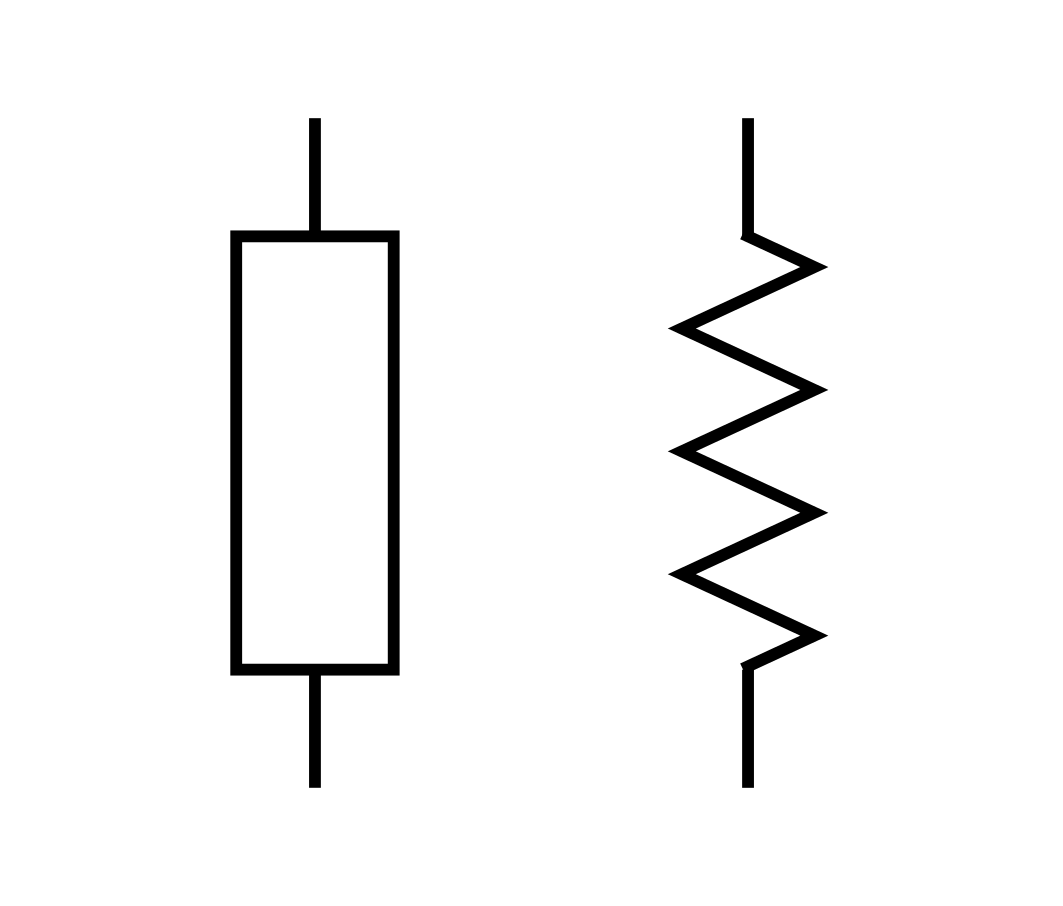
\includegraphics[width=0.5\textwidth]{resistor1}

This is a basic circuit, with wires, a resistor and a battery, to demonstrate V=IR. \href{https://tinyurl.com/27gj49kj}{Link}

In the specific example, we have a resistor of 1 Ohms and a \gls{vltg} of 5V. Therefore, using $V=IR$, we can rearrange to find a current of $I = 5/1 = 5A$. Then we can find a power of $P = IV = 5*5 = 25W$. The simulation shows each of these. Feel free to play around with it and alter values. Instructions for using the simulation program are found (here).

\Examples{Example circuits etc}

There aren't many example circuits using the above knowledge alone. One example would be a heater project. Given you know the available input \gls{vltg}, and the needed thermal load, you can calculate the required heating element resistance.

\Quiz{Quiz}

1. True or false, power draw is always constant for a given resistor, whatever circuit it is in?

2. True or false, resistors are available in a wide range of resistance values, but multiple can be used together to achieve more specific values?

3. True or false, resistors convert electrical energy to thermal energy?

\subsection{Potentiometers}

A potentiometer is a variable resistor acting as a potential divider, using a dial to alter its output resistance. There are many cases where this is helpful, like altering speaker volume, or where \gls{vltg} needs aren't clear or certain. They typically have 3 pins, for the input, ground and output. The input and output together act as a resistor, with a value depending on how the dial is turned.

Digital potentiometers are an example of an integrated circuit (see here), which are programmed to act as a set resistance, using set steps, meaning the same resolution isn't usually attainable.

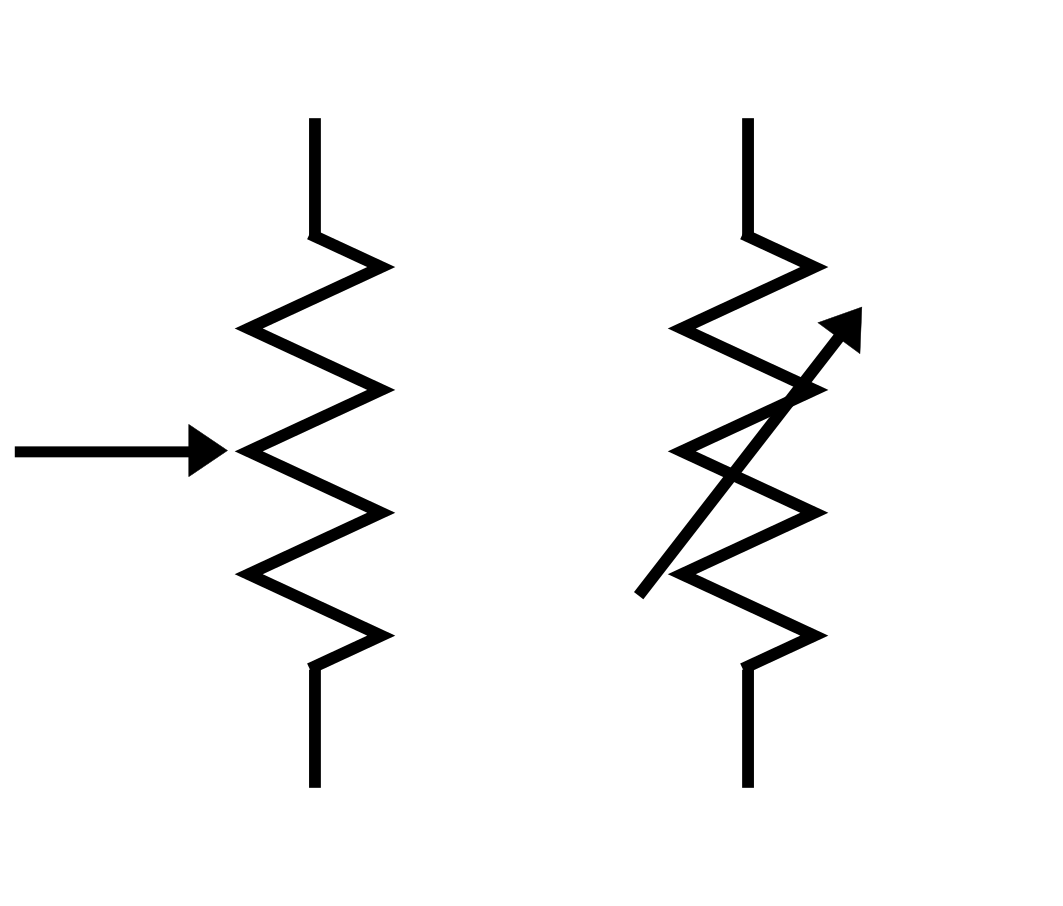
\includegraphics[width=0.5\textwidth]{potentiometer1}

\subsection{Series and Parallel}

You can wire a circuit with parallel and series elements. A series circuit has a single loop, with components connected one after another, sharing a single \gls{vltg}. A parallel circuit can have more than one loop branching out. Each loop has a \gls{vltg} equivalent to the input, with the current split between them, based on their resistance.

Therefore, the \gls{vltg} in a series loop will be distributed based on the \gls{vltg} ratios. For example, there is a 10$\ohm$ and 5$\ohm$ resistor, with a 9V supply, there would be a \gls{vltg} drop of 6V through the 10$\ohm$ resistor and a 3V drop through the 5$\ohm$ resistor. With a total resistance of 15$\ohm$, we can calculate the current to be $V=IR$, $I=V/R$, $I=9/15=0.6A$.

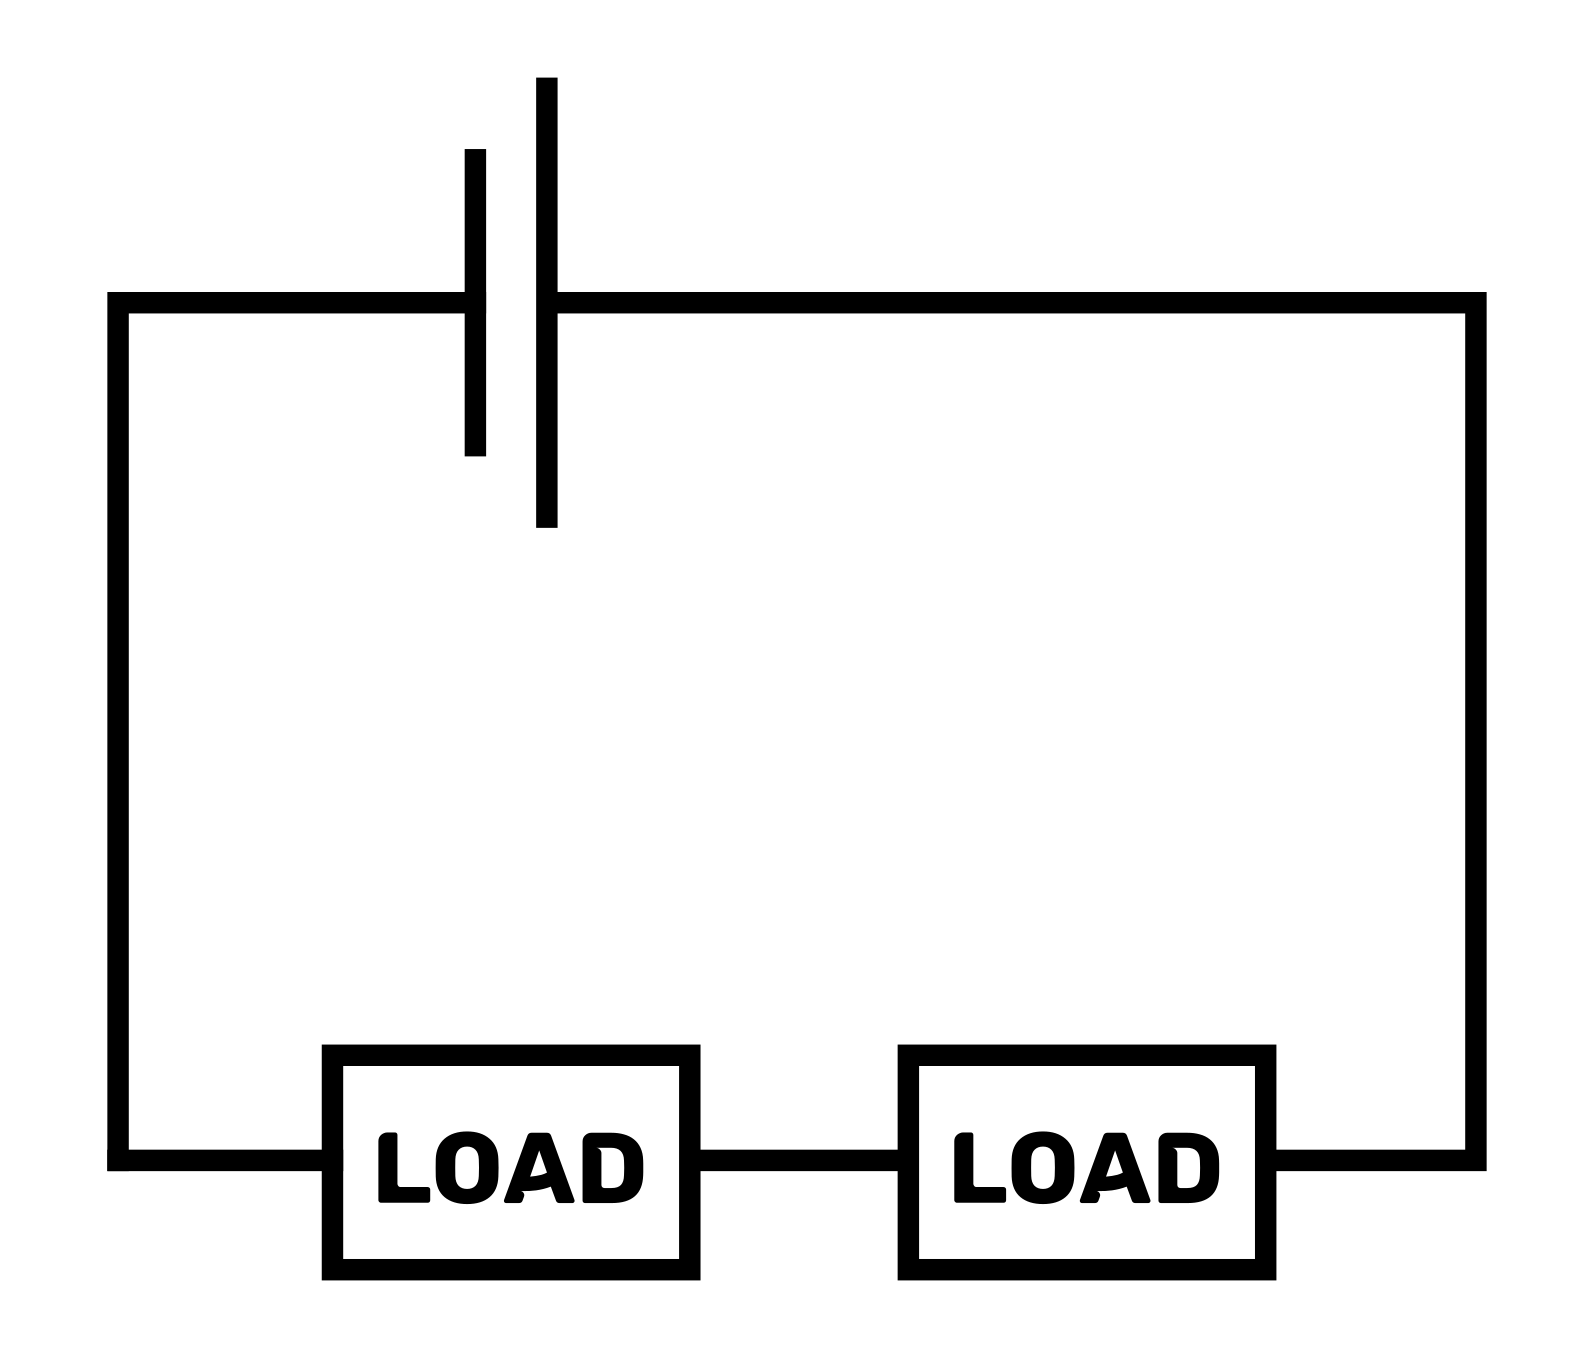
\includegraphics[width=0.5\textwidth]{series1}
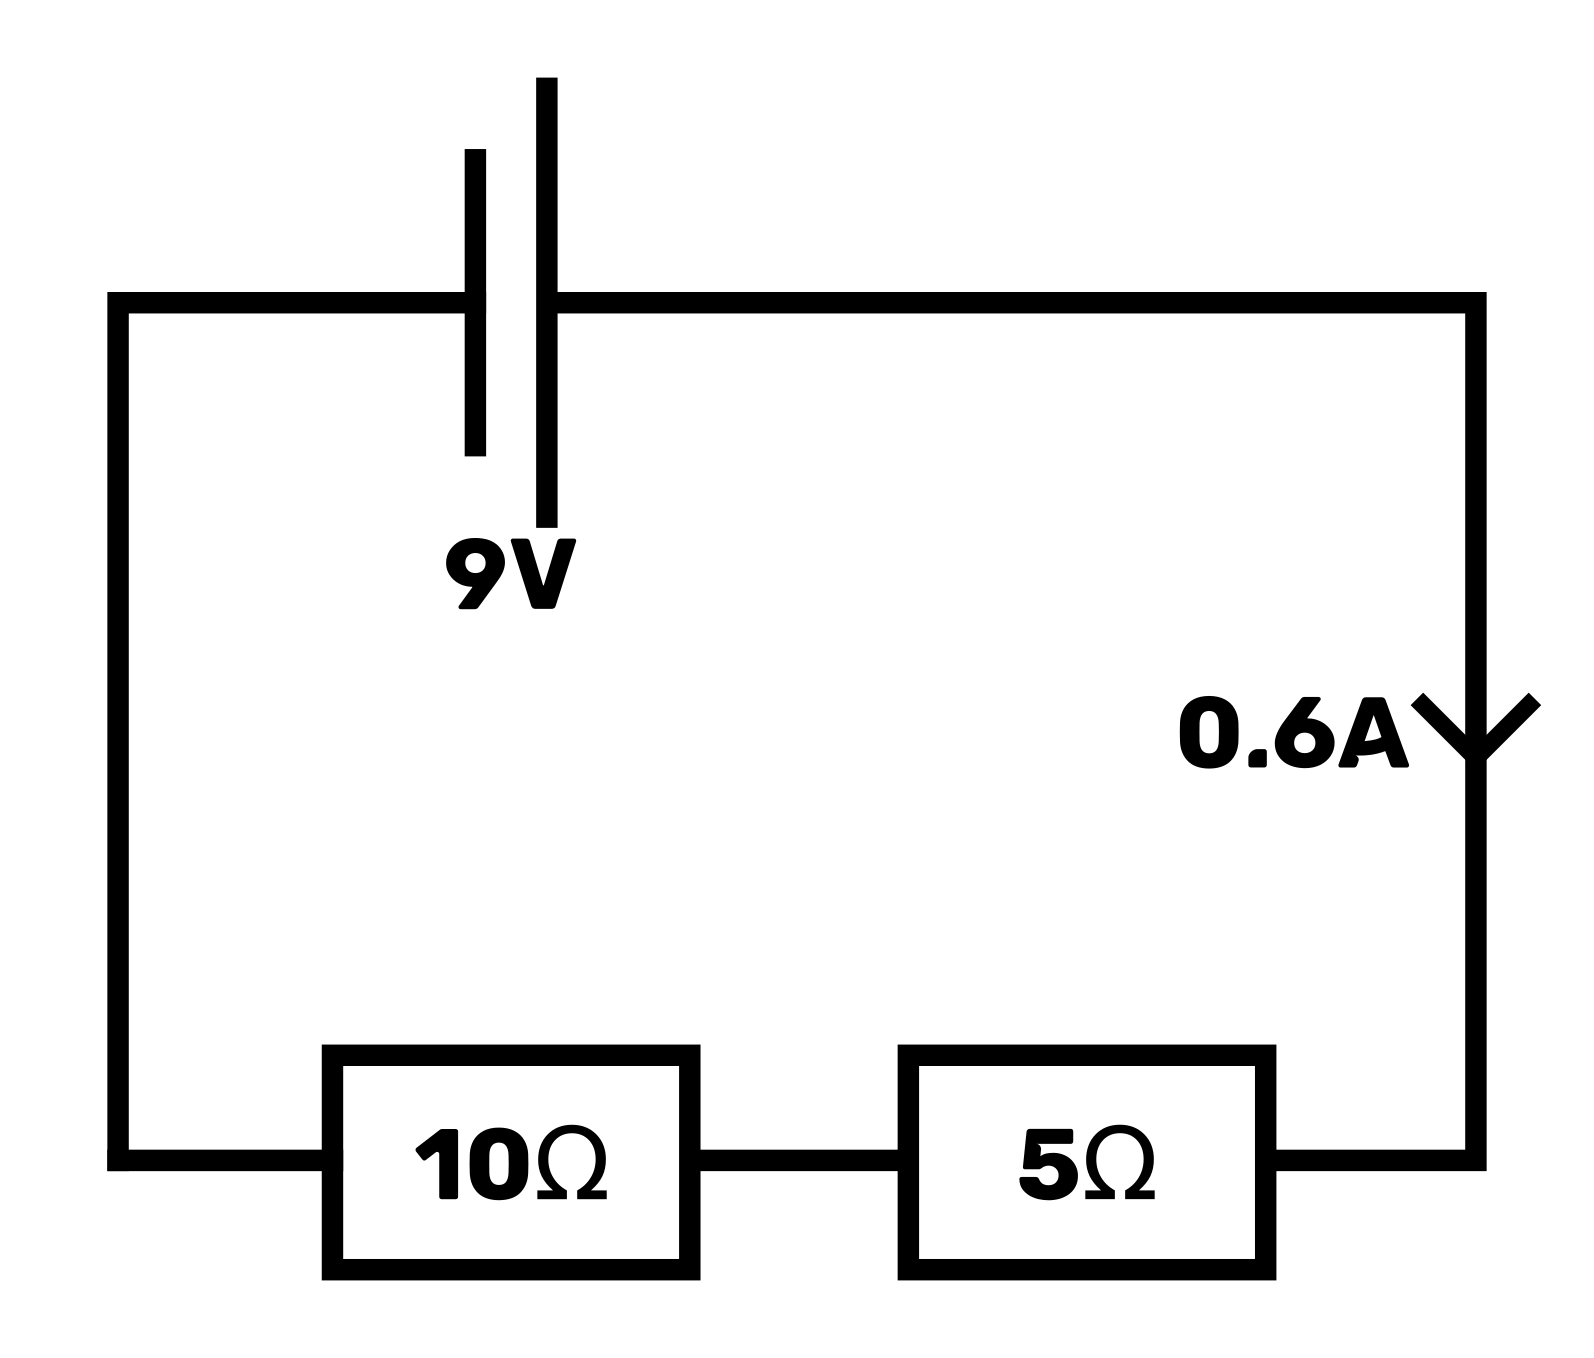
\includegraphics[width=0.5\textwidth]{series2}

A parallel circuit has equal \gls{vltg} across each path, with the current being split. Because of this, resistors in parallel have a total resistance lower than the lowest resistance path.
We can calculate this using the below equation:
\[\frac{1}{R_{total}} = \frac{1}{R_1} + \frac{1}{R_2} + \frac{1}{R_3} + \cdots\]

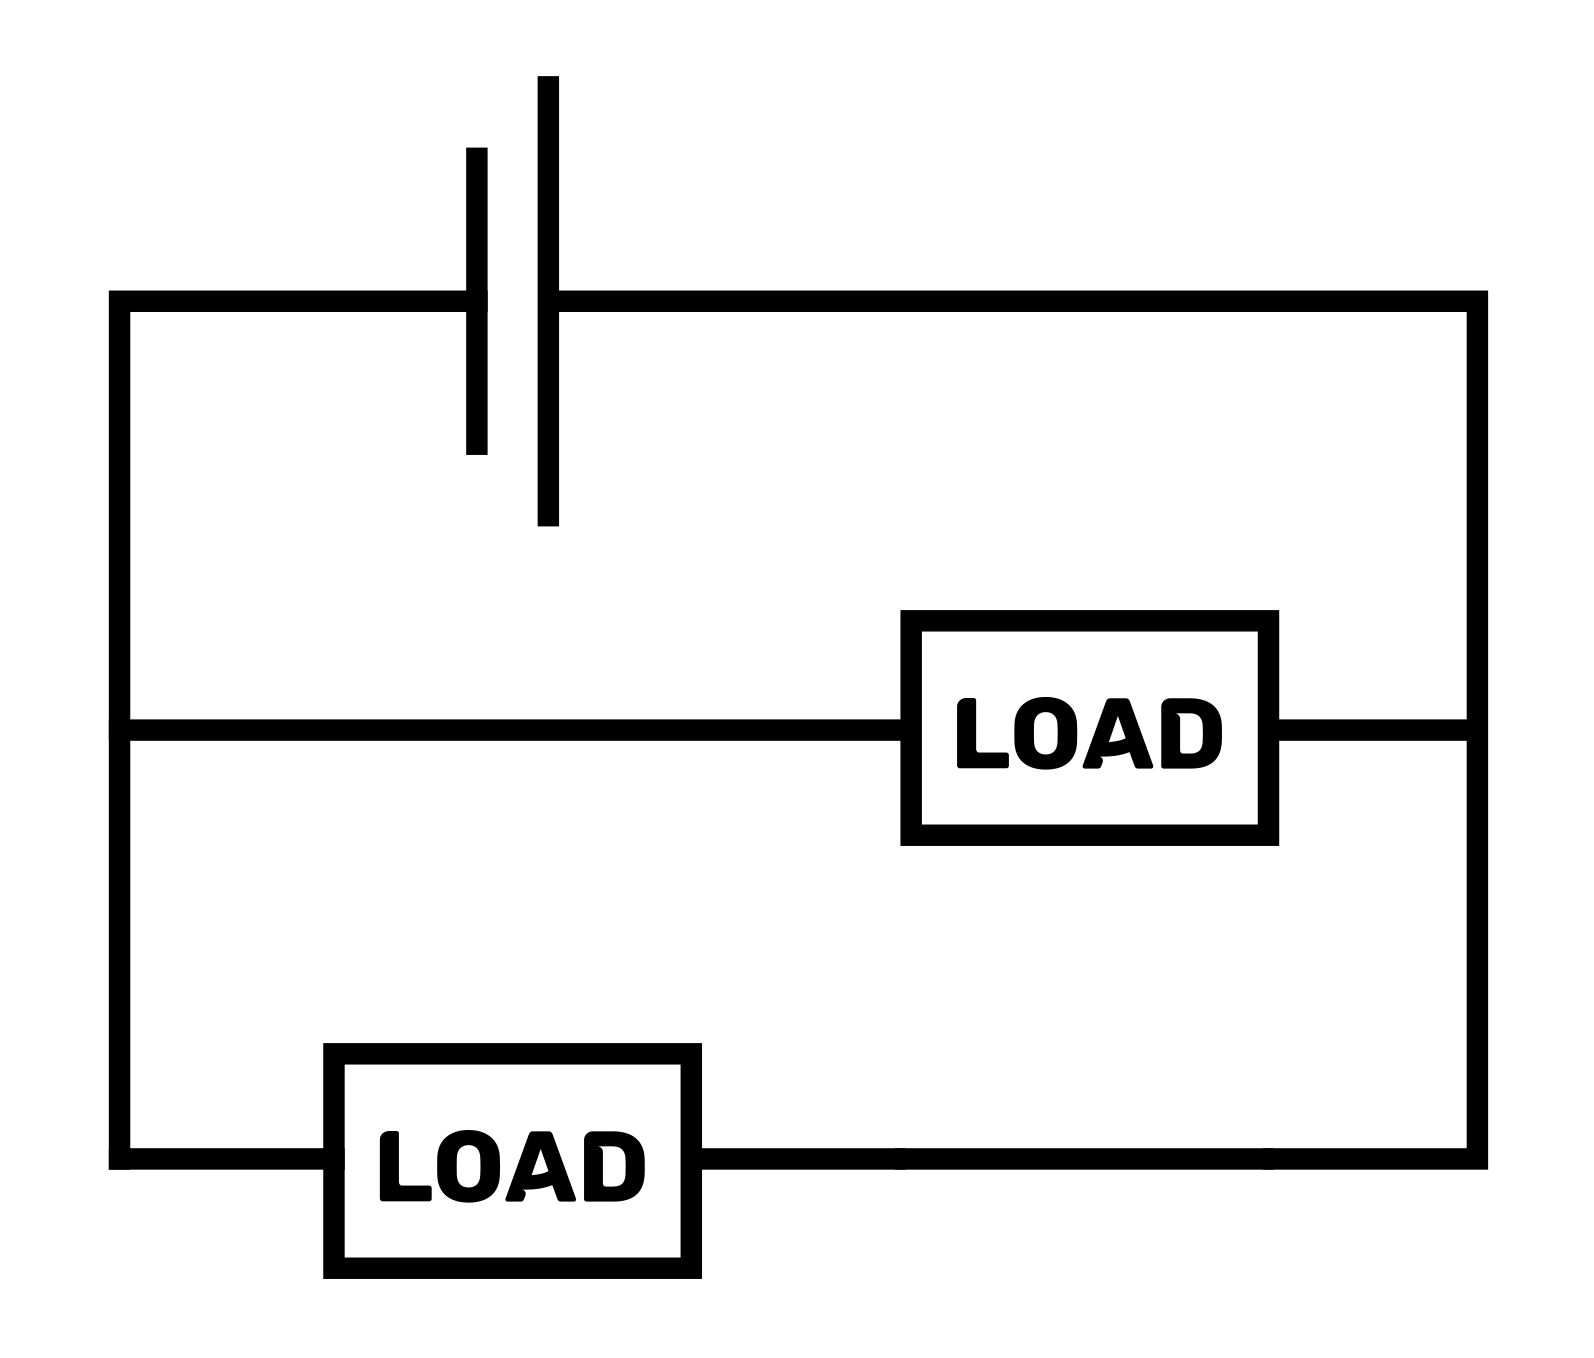
\includegraphics[width=0.5\textwidth]{parallel1}
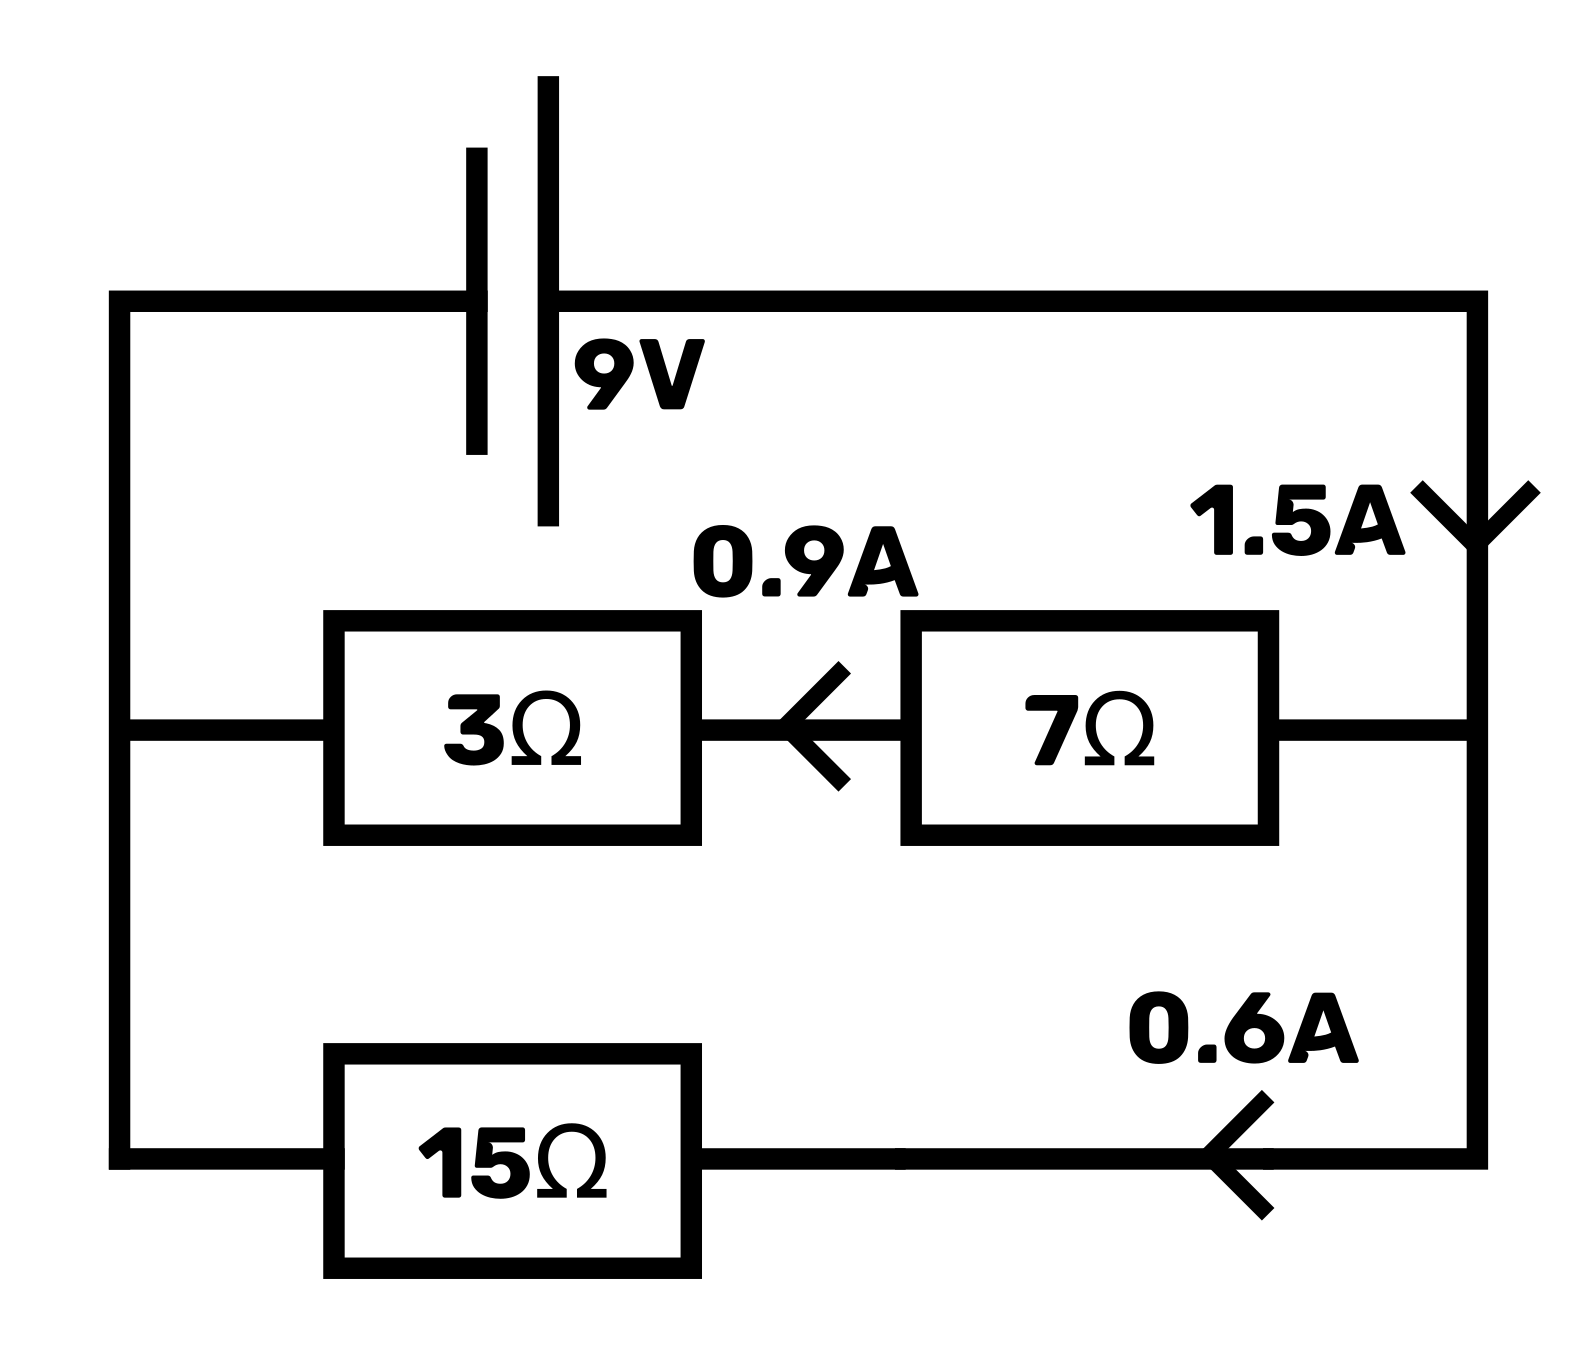
\includegraphics[width=0.5\textwidth]{parallel2}

Therefore, an example with the following circuit with 2 resistors of 3$\ohm$ and 7$\ohm$, in parallel with a single resistor of 15$\ohm$. You first add the series resistors, therefore $R_1$ is 10$\ohm$ and $R_2$ as 15$\ohm$. Therefore, putting it into the equation gives us the below:
\[\frac{1}{R_{total}} = \frac{1}{10} + \frac{1}{15}\]
\[\frac{1}{R_{total}} = \frac{1}{6}\]
\[R_{total} = 6\ohm\]

\Quiz{Quiz}

1. Which of the following statements are true?

a) Current is equal down each path from a junction.

b) Current splits at a path junction, based on each paths resistance.

c) \gls{vltg} is equal down each path from a junction.

d) \gls{vltg} splits at a path junction, based on each path's resistance.

2. What is the \gls{vltg} drop of each component? Also, calculate the power of the circuit.

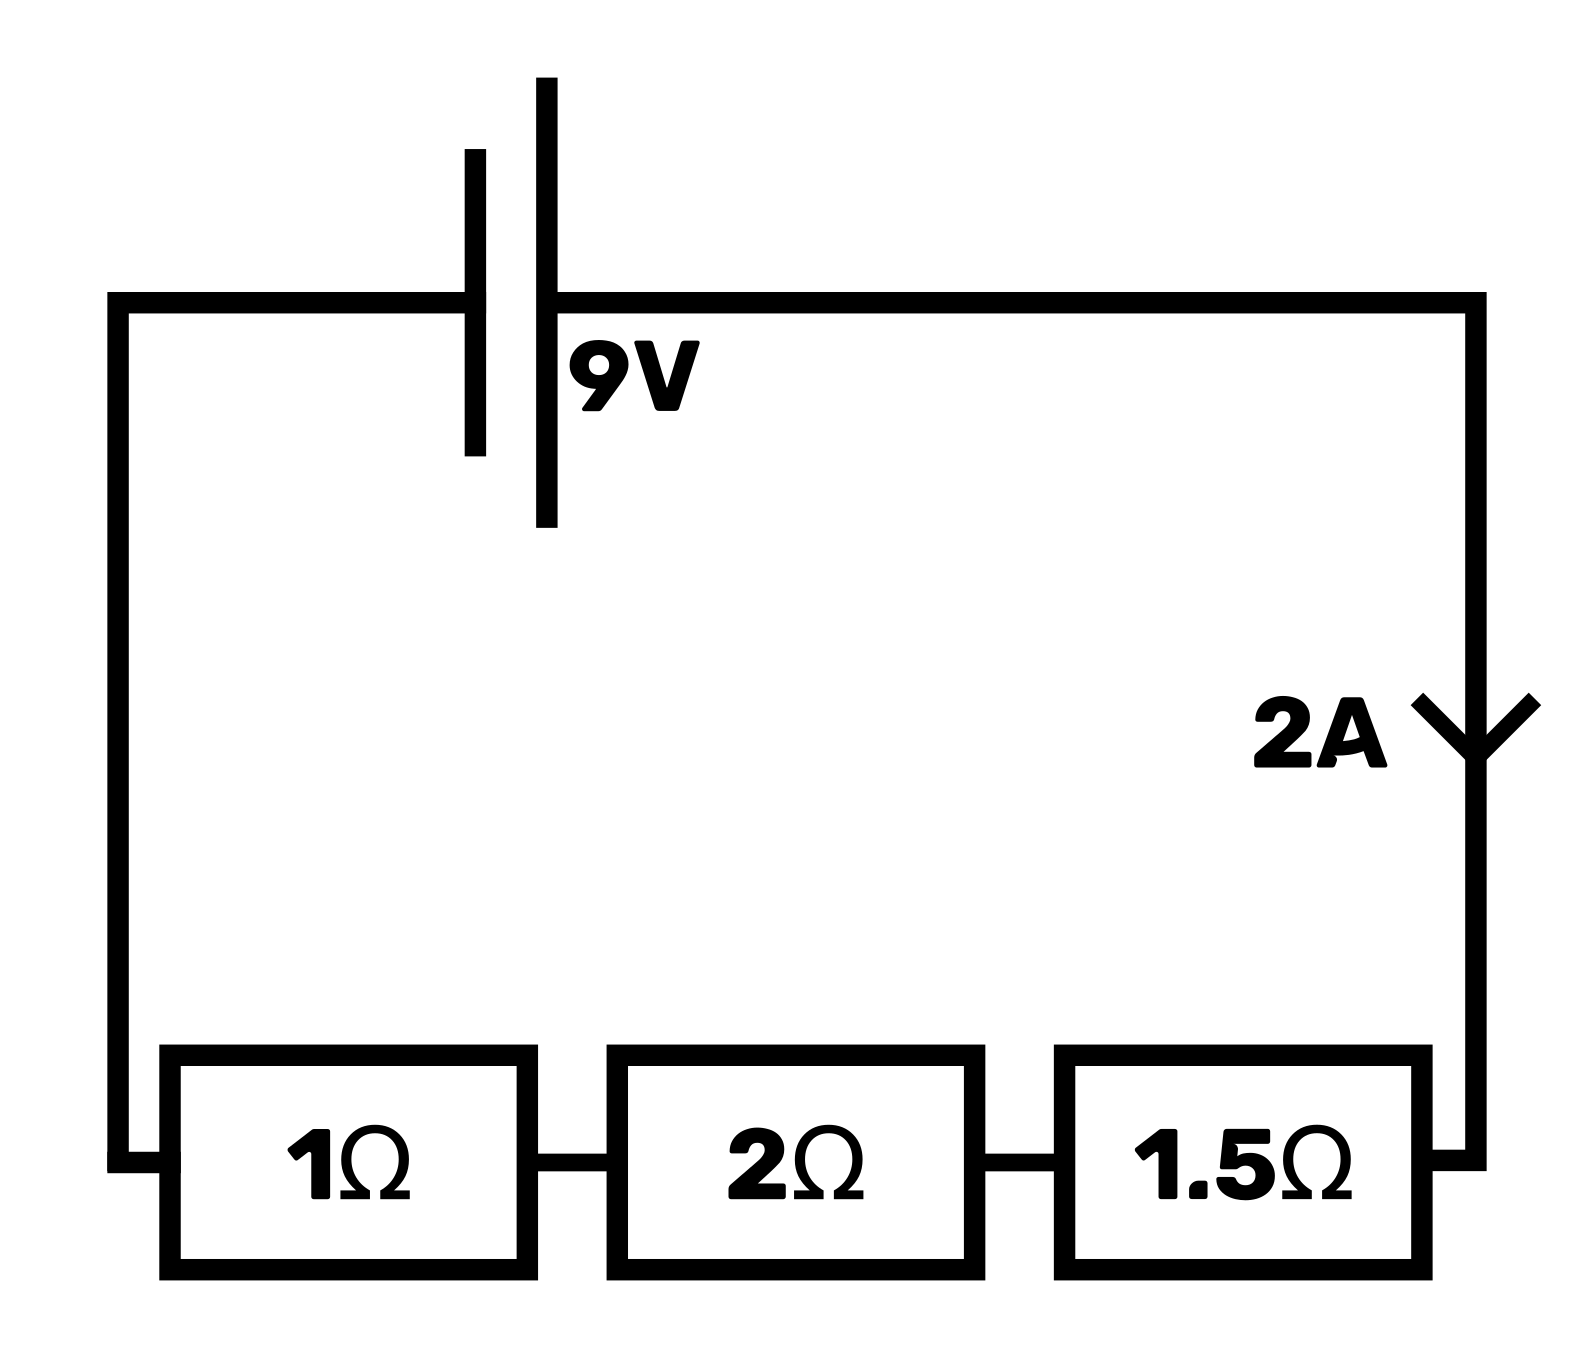
\includegraphics[width=0.5\textwidth]{series3}

3. What is the equivalent resistance of a 20$\ohm$, 100$\ohm$ and 42$\ohm$ component, all in parallel?

4. True or false, the power draw through two  20 $\ohm$ resistors is higher than through a single 10 ohm resistor?

\subsection{Potential Dividers}

Potential dividers use knowledge of both parallel circuits and resistance. As the name suggests, they help to divide \gls{vltg} potential based on the use of series resistors. As stated before, within a series path, the \gls{vltg} will be divided between the components based on their resistance.

\includegraphics[width=0.5\textwidth]{PotentialDivider}

Therefore, if there was an input \gls{vltg} of 5V, and R1 has a resistance of 10$\ohm$ and R2 has a resistance of 3$\ohm$, then the \gls{vltg} seen through the potential divider's output is the below:
\[V_{out}=\frac{(R_1+R_2)-R_2}{R_1+R_2}*V_{in} = \frac{10}{13}*5 = \frac{50}{13}V\]

\Examples{Example circuits etc}

A basic example would be a basic way "dividing" a \gls{vltg}. \href{https://tinyurl.com/27sybjry}{Link}

\subsection{AC vs DC}

AC stands for alternating current, whereas DC stands for direct current. This is shown on a graph with the direction of flow on one axis and magnitude of \gls{vltg} on the other. DC has a constant magnitude and direction of flow. This compares to a sinusoidal \gls{vltg} magnitude with AC, where the flow of current varies in direction. AC is typically given as an RMS \gls{vltg} and a frequency. The frequency is the number of periods that happen per second, typically given in Hz, where the \gls{vltg} is an average value, taking the root mean square. Root mean square (RMS) represents the DC \gls{vltg} that has the same power/ heating effect as the AC circuit. This is seen with power from the grid, with RMS \gls{vltg}s of 230V and frequency of 50Hz in the UK.
Being in AC allows for converting \gls{vltg}s to very high amounts through long distance cables using transformers, to reduce thermal losses due to current.

\includegraphics[width=0.5\textwidth]{acsource1}\includegraphics[width=0.5\textwidth]{dcsource1}

\includegraphics[width=0.5\textwidth]{acwave}\includegraphics[width=0.5\textwidth]{dcwave}

Digital electronics are within the DC realm, but many devices still require AC. It is the standard for energy generation and for how it is sent across the grid. AC is widely used for motors, and where large \gls{vltg} transformations are required, such as microwaves. Semiconductor electronics primarily work within DC.

The course will touch upon ways to convert between AC-DC and the benefits of each for different applications.

\Quiz{Quiz}

1. What is the frequency of AC Electricity from the grid in the UK?

2. What does RMS stand for?

3. Why is AC used within the grid?

\subsection{Capacitors}

\Theory{What are Capacitors?}

Capacitors are another key component. They store energy as Electric Potential, with their \gls{vltg} increasing towards the input \gls{vltg}, as they charge. Therefore, the charge and discharge curve is nonlinear, more similar to an exponential curve.

The unit for capacitance is Farad, with typical values depending on capacitor type, but usually in the uF units or below.

A range of physics based equations will be touched upon now.

Capacitors have a charge relating to their input \gls{vltg} with the following basic equation: $q = CV$.  C is capacitance, q is charge, and V is \gls{vltg}. There is also the formula for energy stored within a capacitor, with the following equation: $E = 1/2*C*V^2$, where E is energy in Joules.

A resistor is usually placed in series with a capacitor to limit the capacitor inlet current. As it charges, the ratio between its \gls{vltg} and the supply \gls{vltg} decreases, along with the charge current, in a curve of reverse direction to the \gls{vltg}.

One of the built in simulation circuits from Falstad is helpful for showcasing the charge and discharge characteristics of a capacitor, by flicking a switch. \href{https://tinyurl.com/2erbz4jy}{Link}

You should be aware of what happens with series and parallel capacitors. The capacitance of capacitors add when in parallel, where in series, it is like resistors in parallel. You can think of it having inverse rules to the resistor. Therefore, capacitors are often used in parallel but less so in series, unless a higher \gls{vltg} is required than their individual rated value. Shown by the equations below:

Series capacitors- \[C_{total} = \frac{1}{\frac{1}{C_1}+\frac{1}{C_2}+\cdots}\]

Parallel capacitors- \[C_{total} = C_1+C_2+\cdots\]

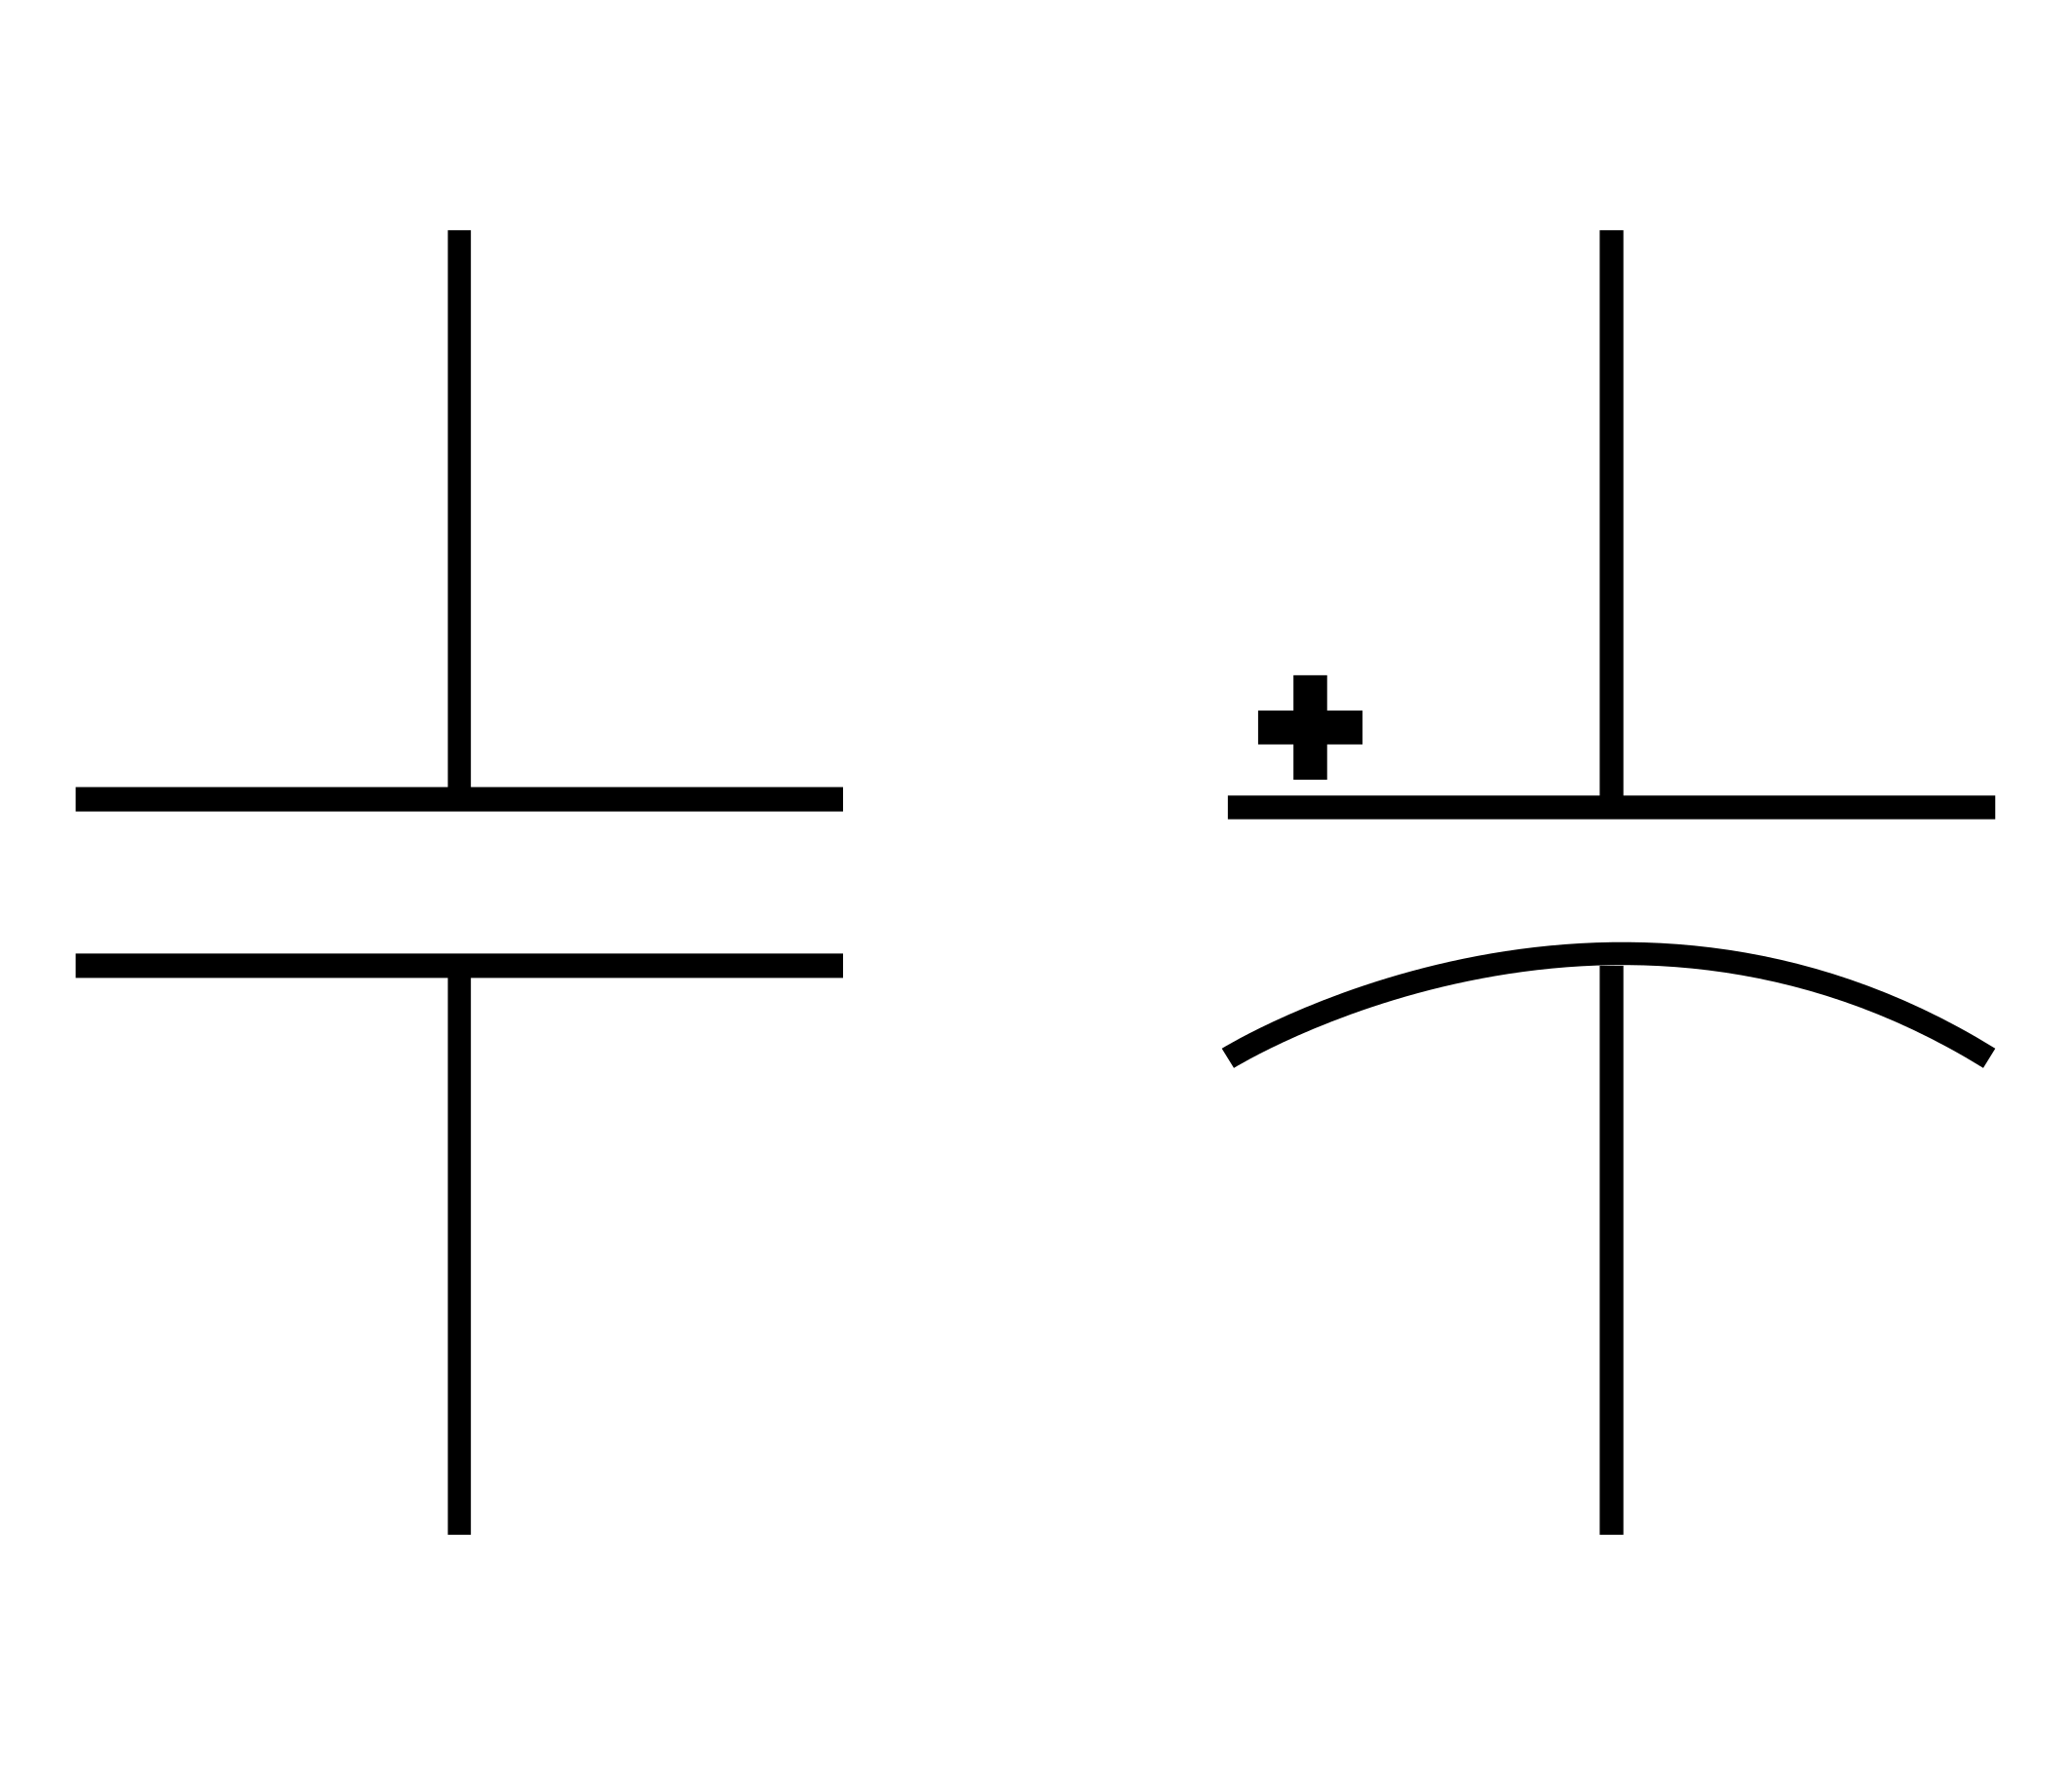
\includegraphics[width=0.5\textwidth]{capacitor1}

\Examples{Example circuits etc}

\Quiz{Quiz}

1. How do capacitors store energy?

a) In the magnetic field

b) In the electric field

c) As thermal energy

d) They do not store energy

2. True or false, a resistor is typically used in series with a capacitor to limit current flow through the capacitor.

3. True or false, 1 Farad capacitors are commonly available.

4. Design a circuit for charging a capacitor at a maximum current of 1A, assuming a source \gls{vltg} of 3V.

\subsection{Inductors}

\Theory{What are Inductors?}

Inductors are another key passive energy storage component. These store energy within the magnetic field, and have a range of uses, often in power electronics.

The unit for inductance (L) is Henry, with typical values depending on inductor type, but usually in the uH or mH units or below.

A range of physics based equations are used to show inductance.

There is the following basic equation: $L = \frac{\Phi(i)}{i}$. There is also the energy formula for calculating the energy stored within an inductor, with the following basic equation: $E = 1/2*L*I^2$.

It is also useful to be aware of the rules for series and parallel inductors. It is like the rules for resistors, although this time being inductance.

Series inductors- \[L_{total} = L_1 + L_2 + \cdots\]

Parallel inductors- \[L_{total} = \frac{1}{\frac{1}{L_1}+\frac{1}{L_2}}\]

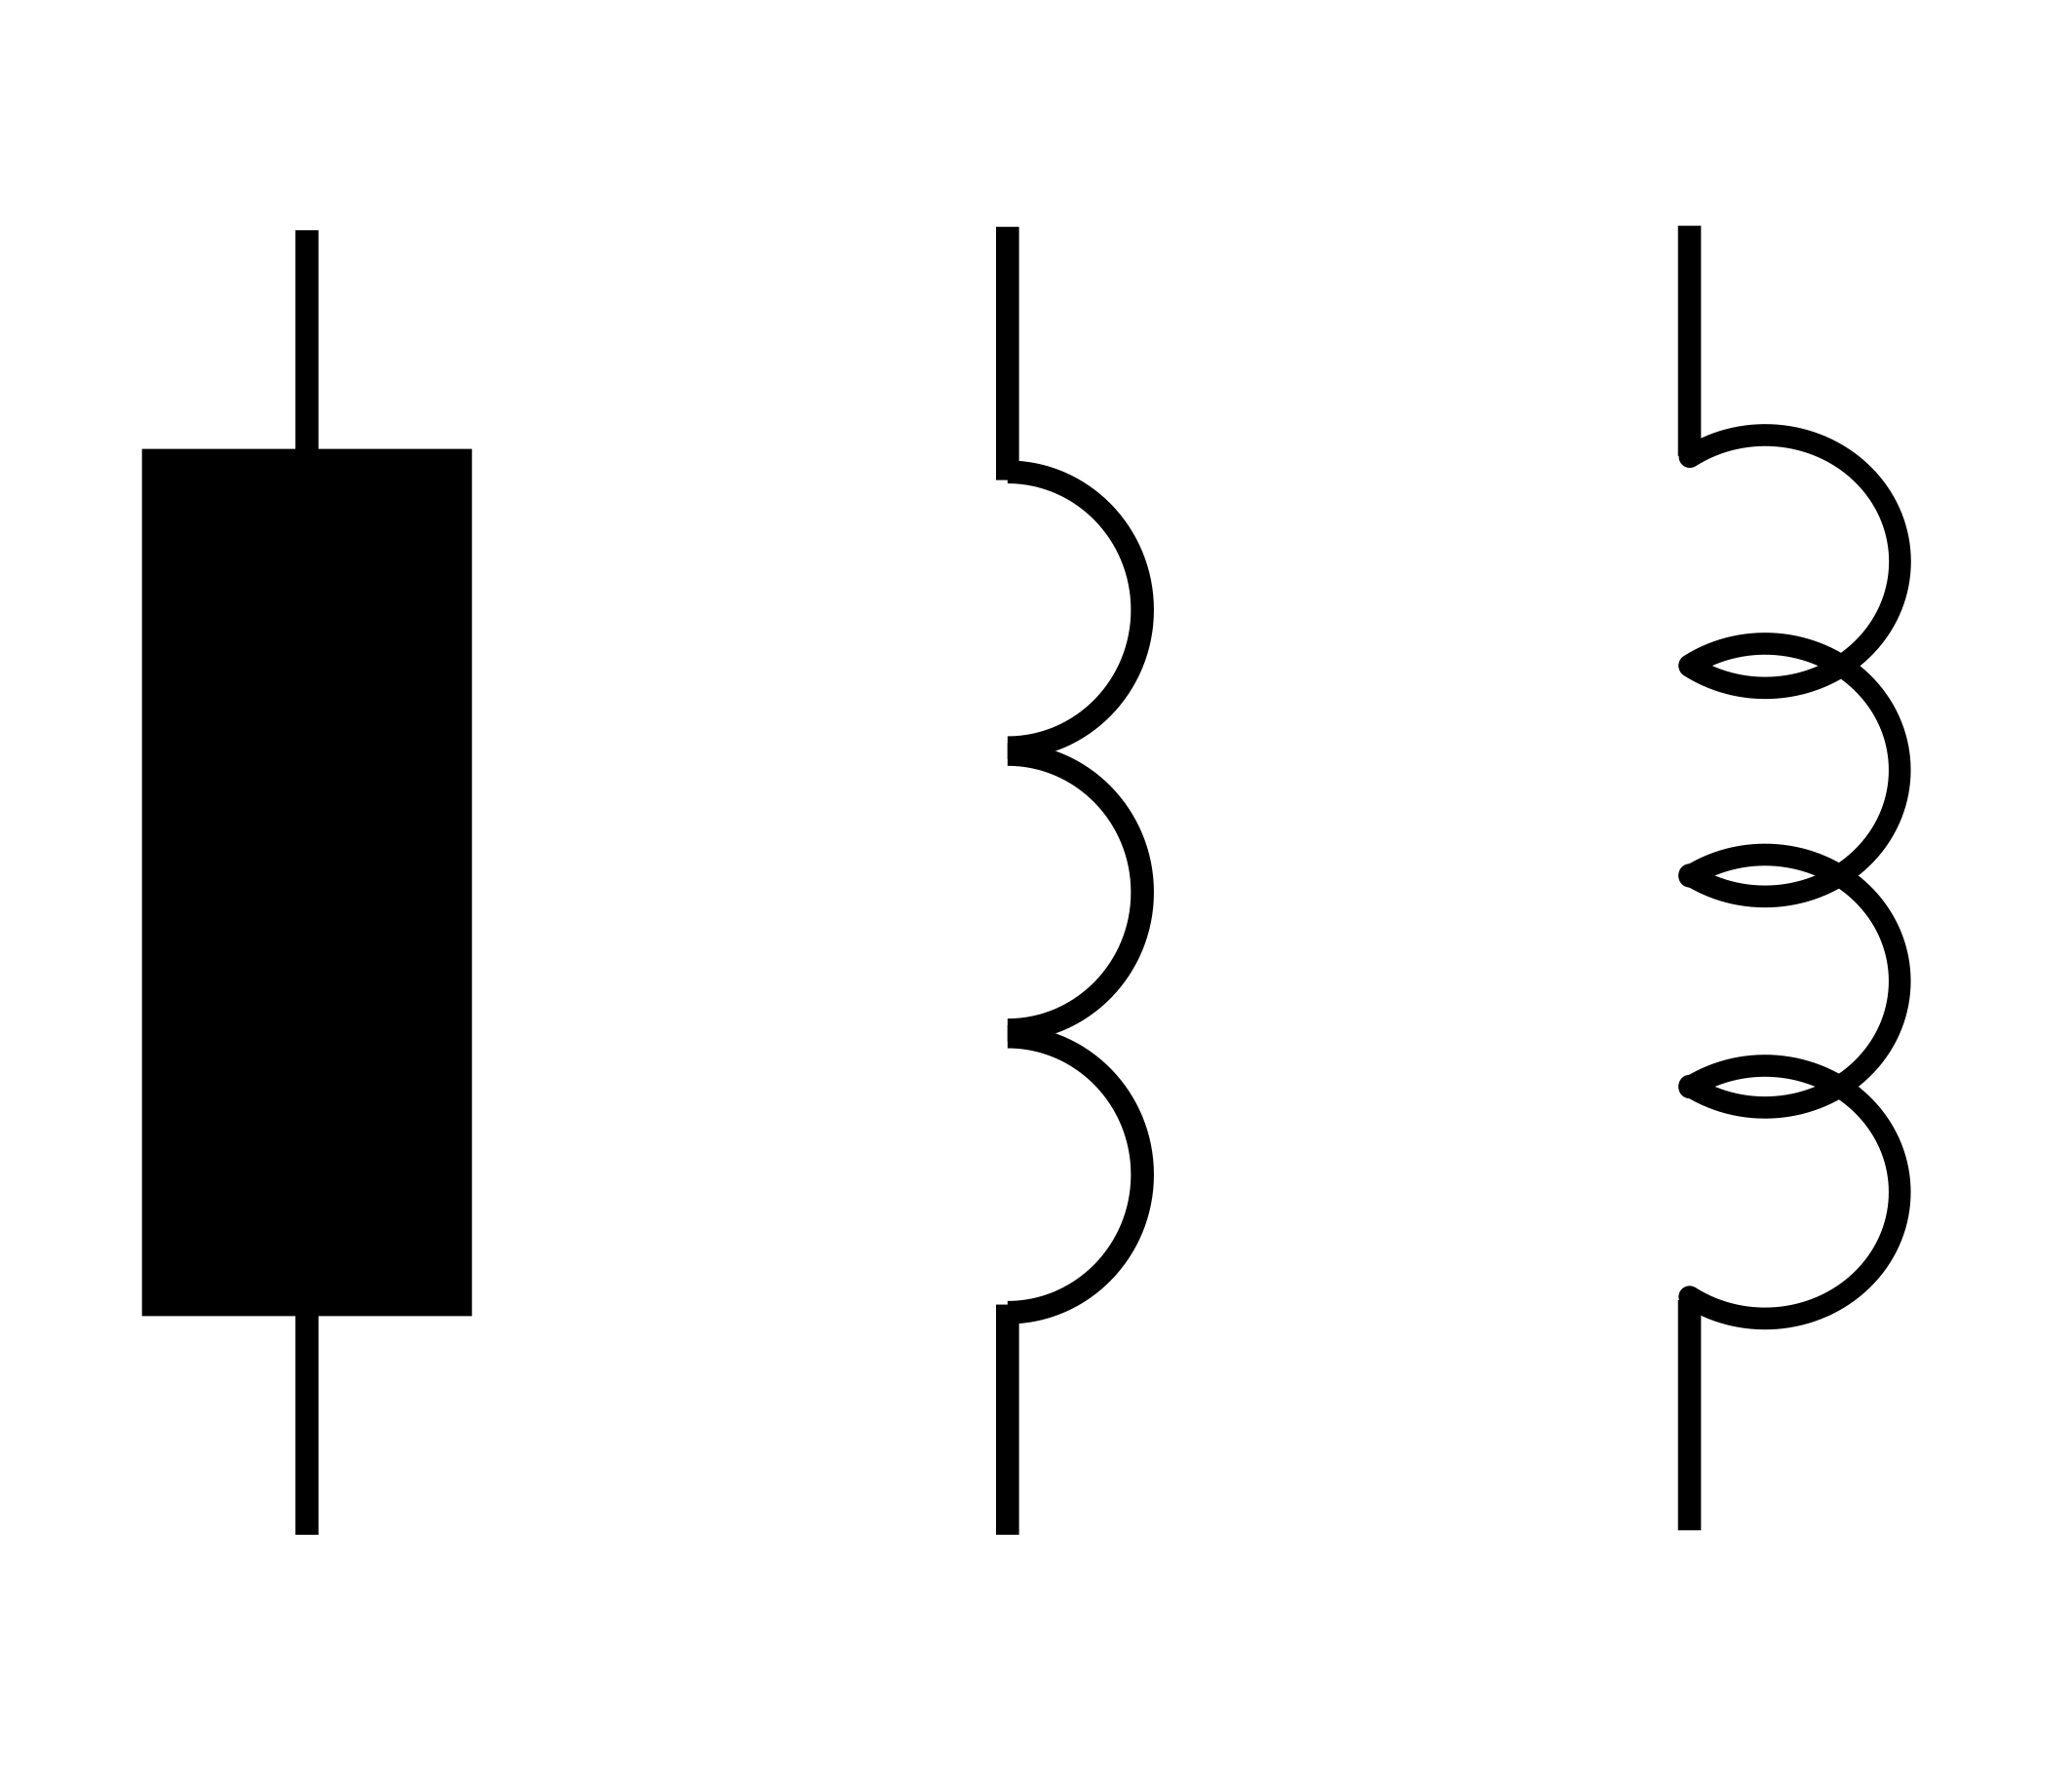
\includegraphics[width=0.5\textwidth]{inductor1}

\Examples{Example circuits etc}

\Quiz{Quiz}

1. What units is inductance given in?

\subsection{Diodes}

Diodes are widely used in electronics. The basic principle of a diode is a device/component which limits how current can flow within a circuit, such as restricting current flow to one direction.
This makes them beneficial for a range of circuits, such as protection circuits, preventing unwanted reverse current flow, which could damage other components or cause unwanted side effects.
They are a simpler examples of a semiconductor, where usually silicon is doped with other atoms to cause a surplus or shortage of electrons, changing the polarity of elements of the material, affecting how current flows through the diode.

There are also Light Emitting Diodes (LEDs), which work through similar principles, but emit light of a certain spectrum depending upon LED selection. There is a \gls{vltg} drop associated with this, but with considerably lower heat output, compared to filament bulbs, which heat filament until it glows.

There is a common formula for calculating the resistor needed for an LED, given you know the \gls{vltg} and current it runs at. This is the following:
\[R = \frac{V_s - V_f}{I_f}\]
Where $V_s$ is the supply \gls{vltg}, $V_f$ is the forward \gls{vltg} (\gls{vltg} drop of the LED) and $I_f$ is the forward current.

Different colour LEDs work at different \gls{vltg}s, so resistors are commonly used to drop the input \gls{vltg} to a level suitable for the LED. The LEDs also help to limit current through the LED. This \gls{vltg} usually is between 1.8-3.3v, and is because of how the semiconductor is doped, as different dopants will cause different wavelengths of light to be emitted.

It is important to consider that diodes have an inherent \gls{vltg} drop, so this needs to be considered, especially when using them with low-\gls{vltg} circuits, as a typical diode can have \gls{vltg} drops between around 0.4-0.7v.

There are many subcategories of diodes. The most common type mentioned above is known as a junction diode. Zener diodes allow reverse \gls{vltg} after a certain threshold is met. A Schottky diode has low \gls{vltg} drop and fast switching. There are also DIACs and TRIACs for AC, allowing some current flow in both directions.

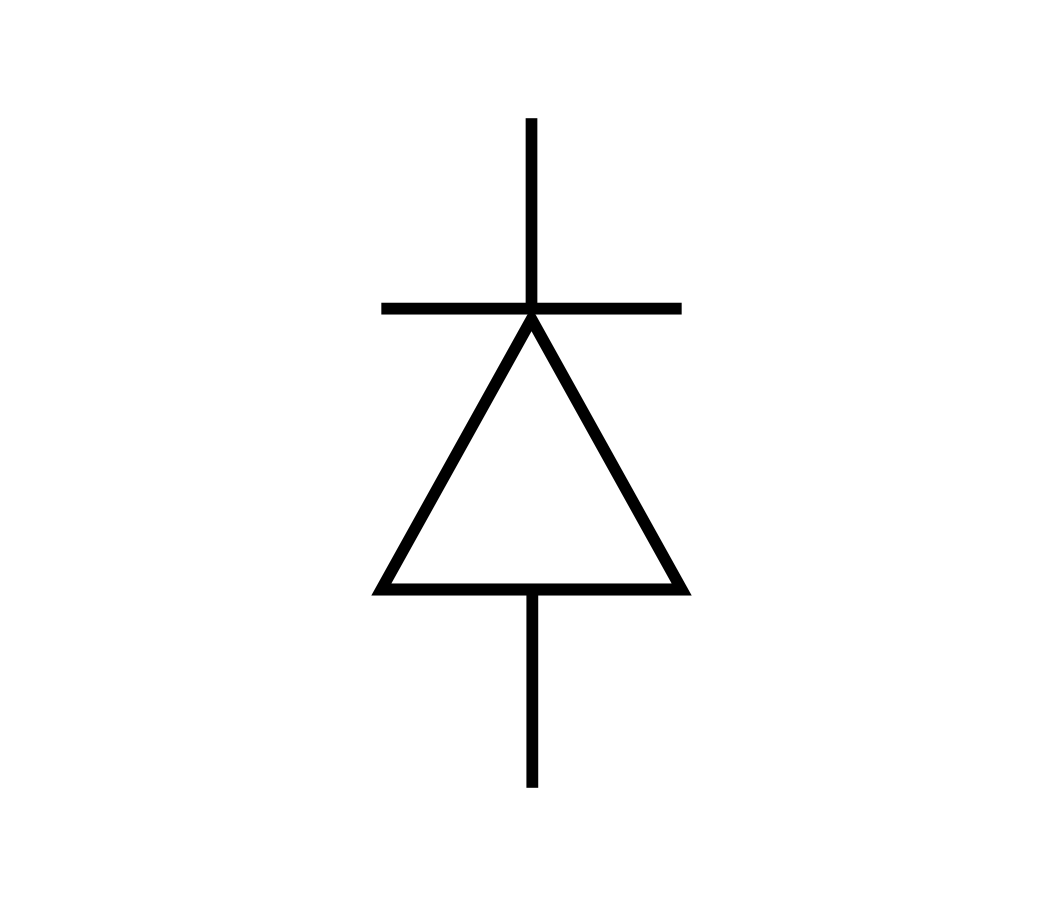
\includegraphics[width=0.5\textwidth]{diode1}
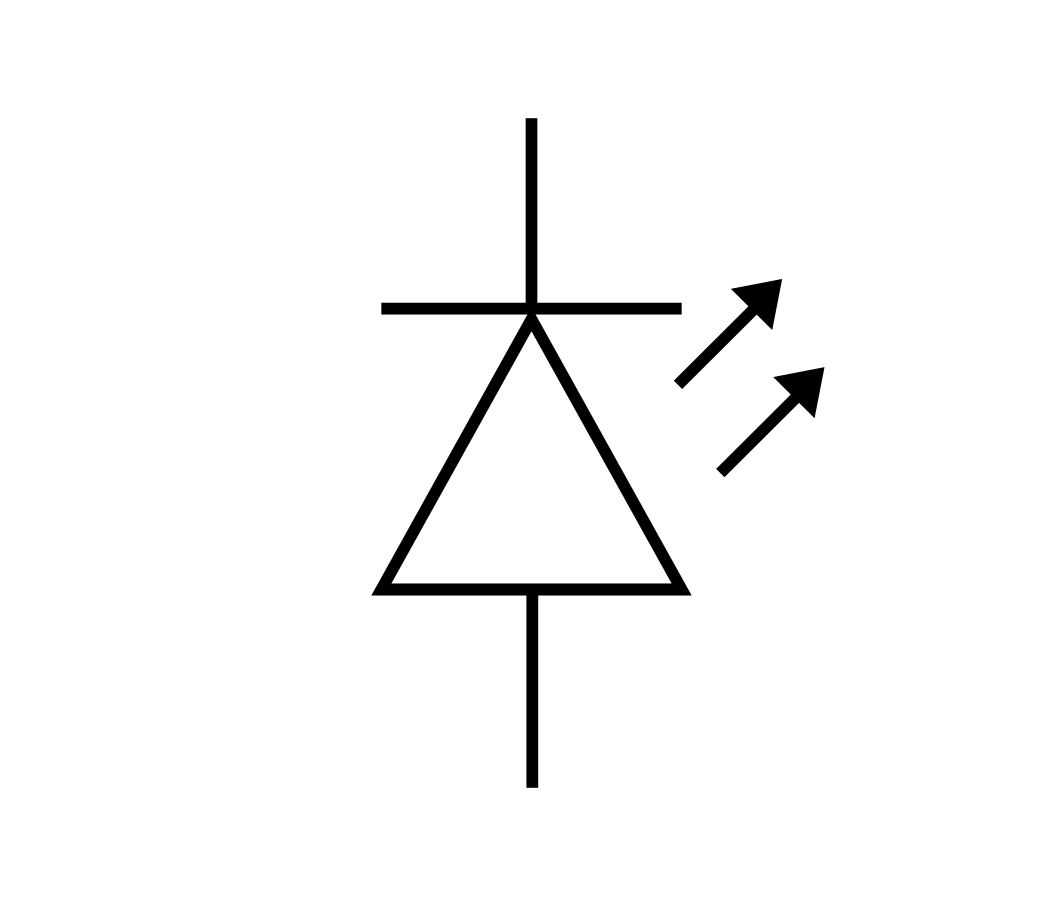
\includegraphics[width=0.5\textwidth]{diode2}
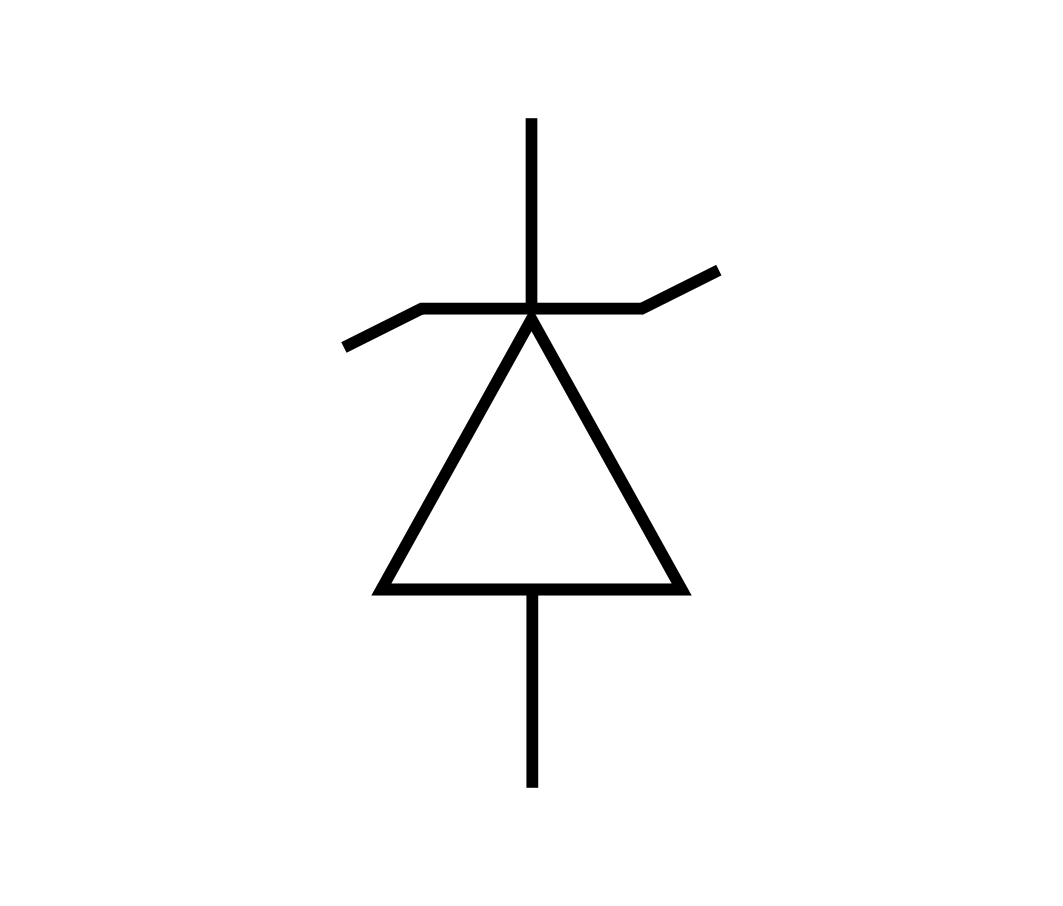
\includegraphics[width=0.5\textwidth]{diode3}
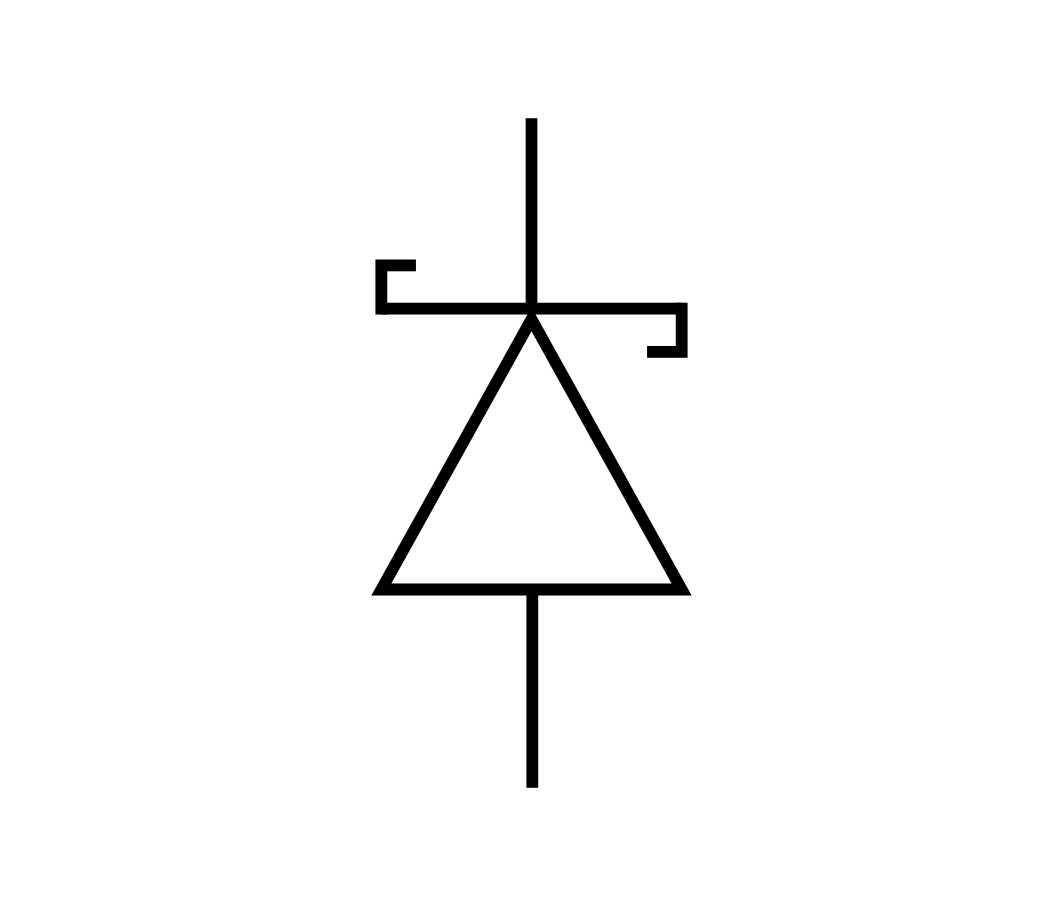
\includegraphics[width=0.5\textwidth]{diode4}

\Quiz{Quiz}

1. Name 4 examples of diodes, and what they do?

2. True or false, diodes always restrict current flow to one direction?

3. You are building a low \gls{vltg} circuit, and need to limit current flow to one direction, but with as low losses as possible. What diode would you recommend?

4. True or false, LEDs can be found in a range of colours, each with differing \gls{vltg} drops?

5. Design a LED circuit, with an input \gls{vltg} of 3V and the LED has a \gls{vltg} drop of 1.8V running at its recommended current of 25mA. What is the total power consumption of this circuit?

\subsection{Transformers}

\Theory{What are Transformers?}

Transformers use the fact that a curren carrying coil of wire will generate a magnetic field, which induces a current in a coil to allow for \gls{vltg}/ current conversion. Think of it as two inductors, coupled through a single core. This is typically a ferritic core to provide a magnetic path to reduce losses. These are often laminated to limit eddy currents, which are loops of current within the core, induced from the magnetic field. Lamination increases the core resistance, reducing the eddy current.

A lot of transformer design is out of the courses scope. We will assume that the transformer is ideal, although in reality, there are losses, leading to efficiencies of upwards of 95\%. This depends on how well suited a transformer is for a design.

Due to current only being induced under a changing magnetic field, Transformers only work with an AC input.

This is the basic set of equations for transformers.

\[\frac{V_p}{V_s} = \frac{I_s}{I_p} = \frac{N_p}{N_s}\]

Where p represents the input/ primary coil and s represents the output/ secondary coil. V represents \gls{vltg}, I represents current and N represents the number of turns/ coils.

There is an inverse relationship between \gls{vltg} and current when there are different coil turns.

There are 1:1 transformers, where no \gls{vltg} or current conversion takes place, but it isolates the input from the output, so is a safety feature often used in products. These are known as isolation transformers.

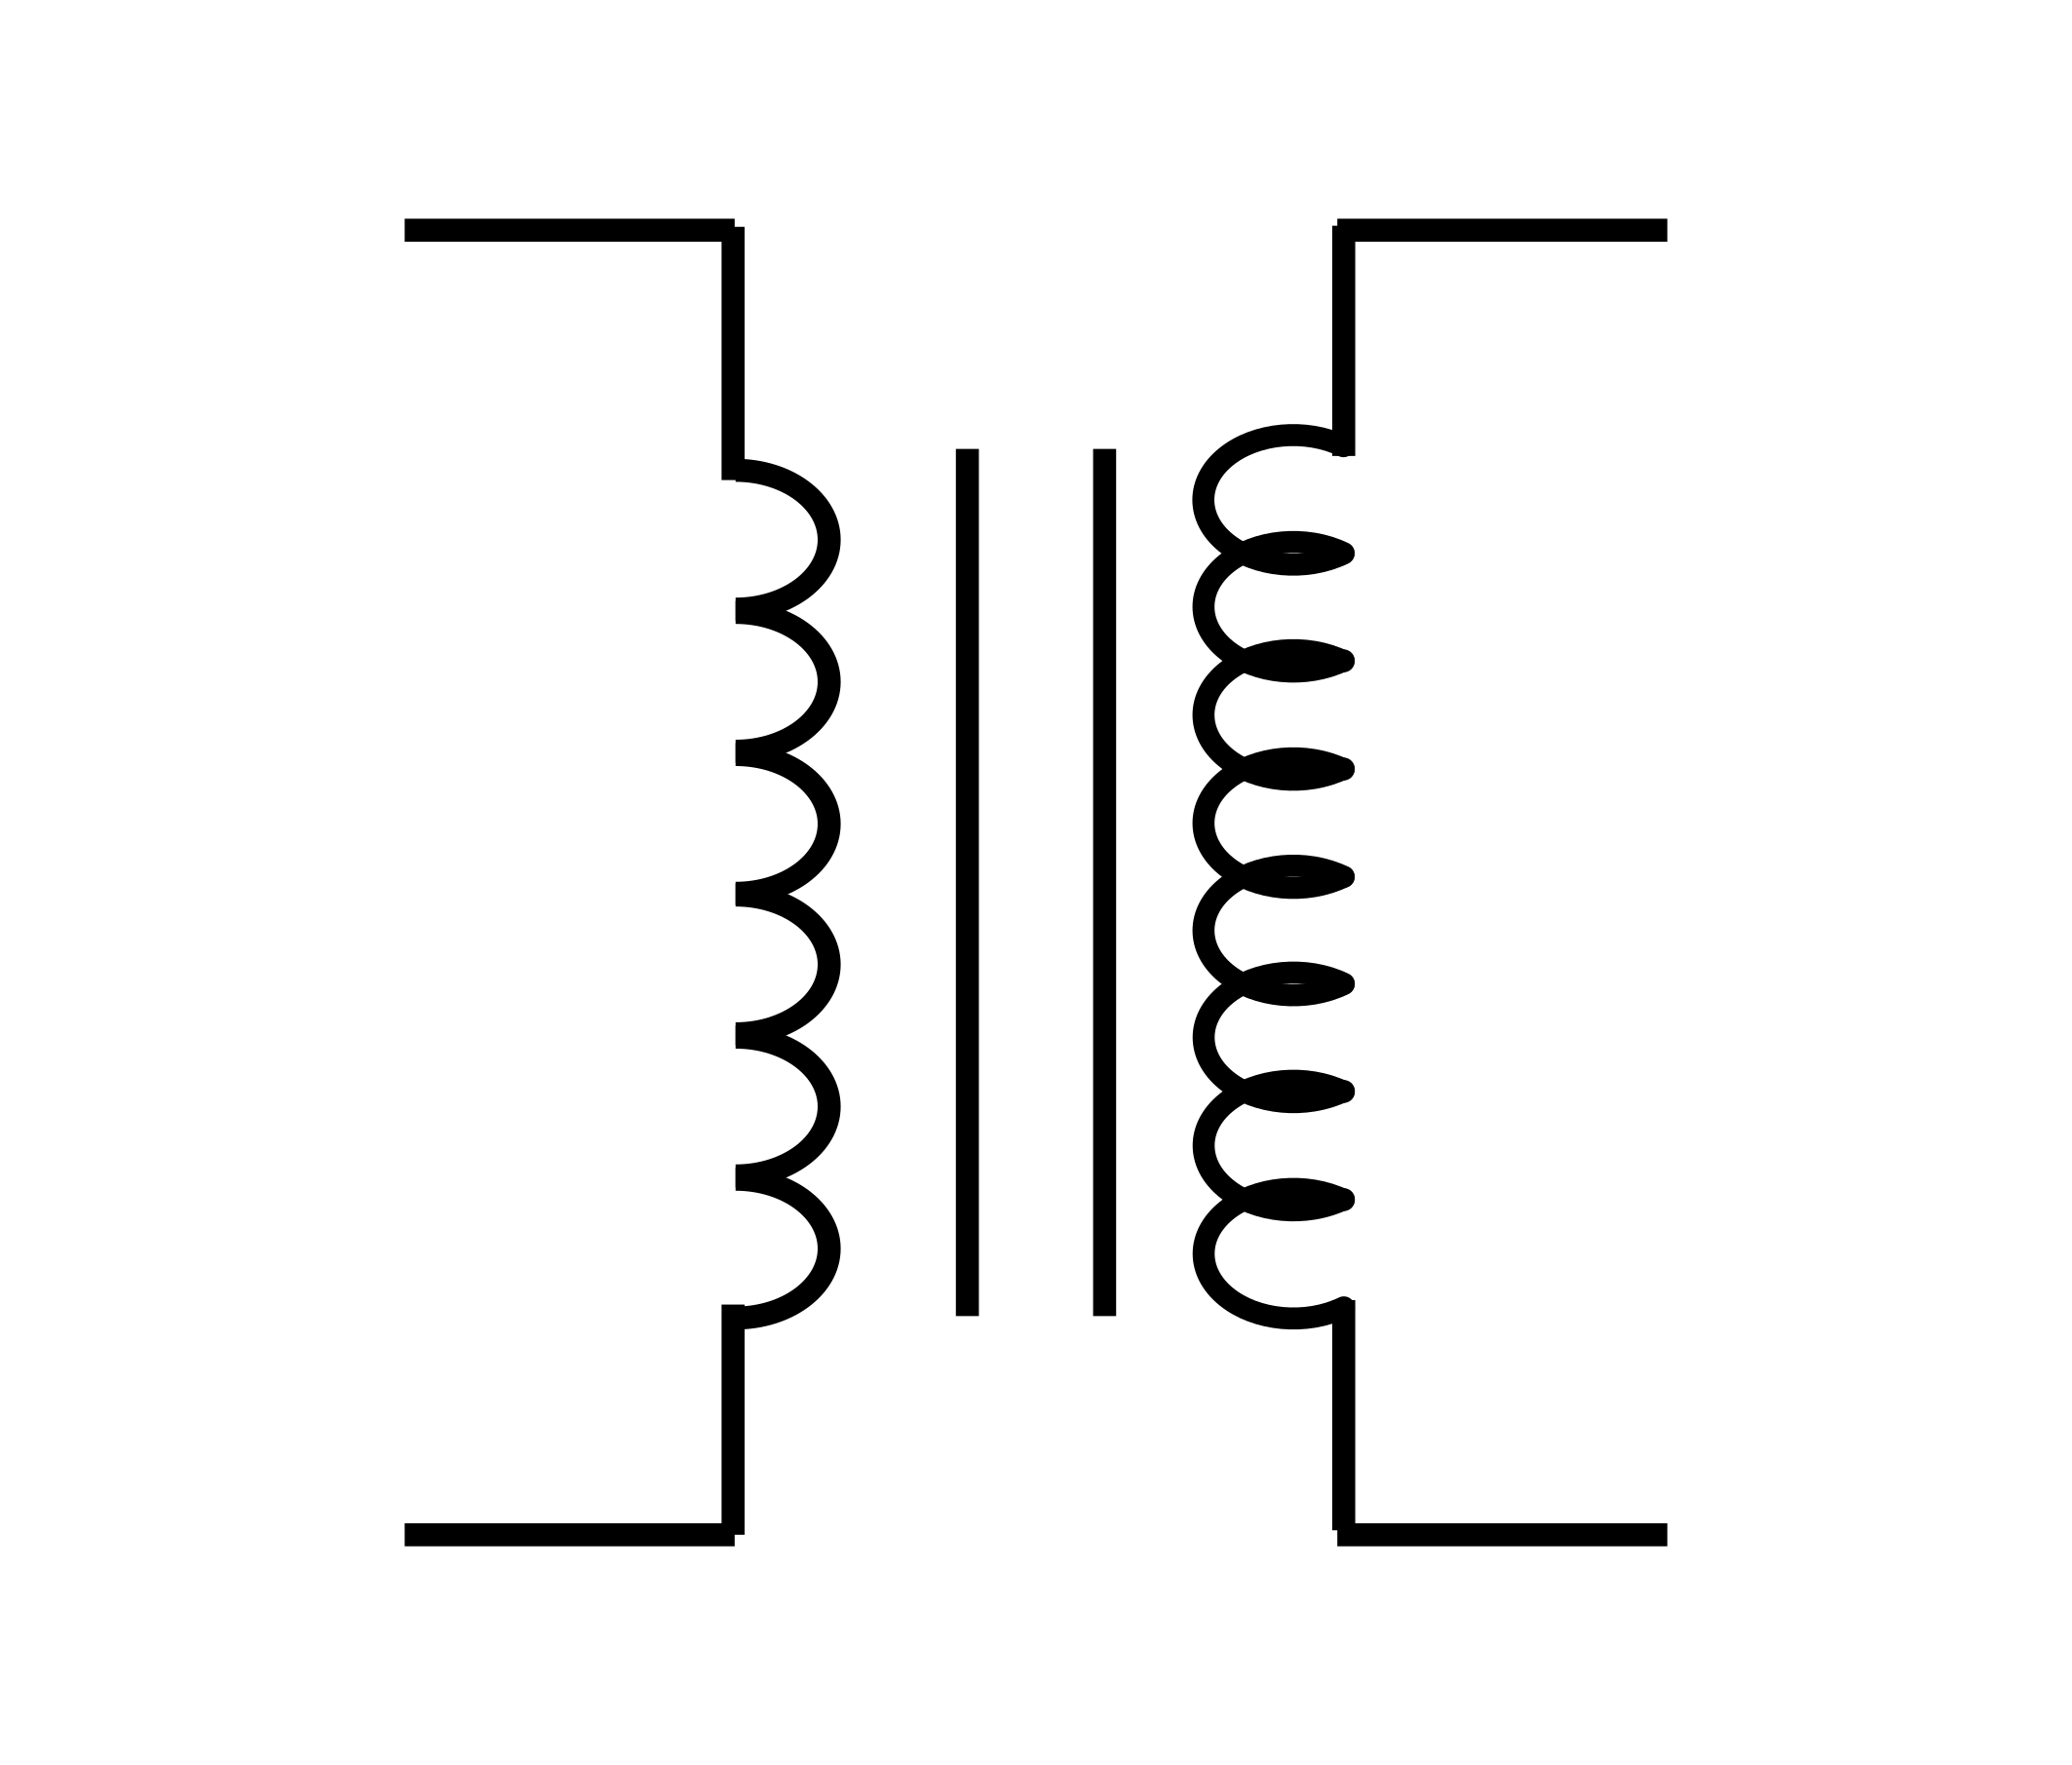
\includegraphics[width=0.5\textwidth]{transformer1}

\Quiz{Quiz}

1. Why are transformer coils often laminated?

2. A transformer with a 240V RMS input with a peak current capability of 0.1A, with 100 turns on its primary side, needs to supply a 12V RMS circuit. How many secondary turns are required, and what is the peak current that could be supplied to the output circuit?

3. Why are isolation transformers used?

\subsection{Analogue vs Digital}

It is important to be aware of differences between analogue and digital. Analogue refers to a wave, with the fundamental characteristics of wavelength, frequency and magnitude. This value can vary considerably within a period, which is particularly useful for some applications.

On the contrary, digital is represented with either 1 or 0 (off or on). As already touched upon, the entire field of modern digital electronics is based around semiconductors, which form switches.

Signals can be sent through both methods, with a range of benefits and negatives. A lot of data can be shown in a single analogue signal, although it can be difficult to accurately read. Whereas, DC deals with two distinct boundaries, so although many more "pulses" are required to output the same amount of data, it is more reliable and easier to use/ read within logic based processing/ boolean algebra, which is touched upon later on in the course.

\gls{snsr}s are often read using analogue methods, where there is an induced or dropped \gls{vltg} which can vary in magnitude. This would need to be converted to a digital value for microcontroller use. A combination of digital 1/0 can be binary, which means a \gls{vltg} value can be represented as a binary combination of 1s and 0s. An ADC is an IC which does this conversion.

\Quiz{Quiz}

1. For a wire communicating over a long distance, would you recommend that an analogue or digital signal be used?

2. Can equivalent numbers be represented with analogue and digital, along with some processing/ data conversion?

\subsection{\gls{snsr}s}

\Theory{What are \gls{snsr}s?}

\gls{snsr}s are likely to be a key component or module you use in your research, so understanding how they work and your options is important. Key aspects of \gls{snsr} theory are discussed here, with more in the further reading section.

This is split into several sections, covering some of the major \gls{snsr}s, with more detail on \gls{snsr}s likely to be used within chemistry related projects.

\gls{snsr}s typically use resistance, capacitance or inductance to take a vast range of measurements, often using a MicroMechanical system (MEMS) to allow for this.

Temperature sensing can be done with a range of different methods, and is likely to be important. The most common \gls{snsr}s are analogue ones, where the components resistance changes along with a temperature change, although there are digital \gls{snsr}s for this too. There are 4 major categories of temperature \gls{snsr}, which we will quickly touch upon each. There are thermocouples, RTDs, thermistors and specific digital ICs.

Thermistors are common, and are divided into NTC and PTC, with NTC more common. NTCs have a decreasing resistance compared to temperature, and will have a resistance rating for 25\degree C typically along with a value for how much their resistance changes per degree. Therefore, utilising a circuit to measure this resistance allows for a relatively accurate temperature to be read. In comparison, PTCs have a positive temperature coefficient.

RTDs are similar in their operation to thermistors, but are meant for a wide range of temperatures, upwards of around 600C. Many consist of a length of thin wire wrapped around a ceramic or glass core.

A thermocouple consists of two differing conductors which generate a temperature dependant \gls{vltg}. They have the highest temperature range of temperature \gls{snsr}s, upwards of around 1800C.

Digital temperature ICs will measure a temperature and report the data through a specific protocol, which is discussed further (here).


Humidity \gls{snsr}s may be used along with temperature \gls{snsr}s, in a single package. The output can be digital or analogue. A couple of common digital examples include the DHT11, DHT22 and AM2320.


There are many \gls{snsr}s for detecting compounds in the air, important for atmospheric research. Usually these are doped so that a higher concentration of a certain gas, such as carbon dioxide, induces a \gls{vltg}. Because of the calibration involved and comparison with data, they are often complex ICs, which communicate via a protocol such as I2C or SPI to a microcontroller, discussed in the protocols section. Although certain \gls{snsr}s may leave the conversion to the user. More modules are appearing in the market, helpful for taking more reliable measurements.


Photoresistors use a similar method for light, where a resistance is associated with pitch black, and separately for light. Therefore, an estimated light intensity will be attained, with a given \gls{vltg}. There are also photodiodes and photoresistors, each with their own benefits, like higher response rate, or lower costs.


There is a range of movement based \gls{snsr}s, which will quickly be touched upon. You are unlikely to need to use these much.

One of the main cheap and widely used range/ movement \gls{snsr}s is an Ultrasonic \gls{snsr}, which has an ultrasonic transmitter and receiver. This uses knowledge of the speed of sound, to measure the time it takes for sound to hit a surface and reflect, to then calculate a distance value.

There are also LiDar \gls{snsr}s, which are similar but known to have higher precision, which use a singular beam of light, and calculate its time of travel. These are also known as Time of Flight (ToF) \gls{snsr}s.

The motion based \gls{snsr}s discussed above are ones that are contactless, but there are also contact based \gls{snsr}s, which a potentiometer could be an example of, using its resistance based on a linear or rotational movement as a measurement of movement.

\Quiz{Quiz}

1. What is the difference between a NTC and a PTC thermistor?

2. What type of temperature \gls{snsr} would you choose for a furnace, with temperatures as high as 900\degree C.

3. If you needed to precisely measure a distance, what would be a good \gls{snsr} choice?

4. Name a couple of protocols that \gls{snsr}s may communicate with?

\subsection{Mechanical switches}

Switches are used as input devices, where depending on being open or closed, will allow power transmission or not, by opening or closing a circuit. These can be split into many types, such as typically open switches unless pressed, typically closed switches unless pressed, or those which switch between open and closed when pressed, and switches which you can switch to close several sets of pins/ connections.

This section will quickly talk through a few different switches/ buttons, their names and uses.

There are different switches that fit into different classifications, which will briefly be discussed.

Single Pole Single Throw (SPST) switches are ones which connect or break a connection between two single wires/ points/ terminals.

Single Pole Double Throw has a single input but two outputs which can be switched between.

There is then also Double Pole Single Throw, which is a combination of two SPSTs and Double Pole Double Throw, a combination of two SPDTs.

Now onto the different types of switch. They can mainly be split into several types, being the below:

Push button- A typical button, some of which will stay closed/ pressed until pressed again, when others such as momentary push switches will only be closed as they are pressed.

Slide switches are flicked into set position, which can be two positions or multiple.

Toggle is a slight adaptation of slide switches, flicking a centred switch from one angle to another, otherwise working through similar means.

Rotary switches can twist to connect a pin with a range of other pins depending where it is twisted to.

You may have a range of switches, such as a few slide switches packaged together in DIP format.

\subsection{Digital switches/ Transistors}

Switches are widely used within electronics and are what led to the field of digital electronics. Microcontrollers may use millions of switches on a single silicon die, where discrete switches are mainly used for power electronics.

Switches are important to have control of a circuit. These are discussed in greater depth later, but they usually have an externally triggered gate, which closes a circuit. Think of a switch as a tap that allows or restricts water flow. The vast majority of these are semiconductor based, due to the low losses involved, although they are limited to DC function.

This document quickly talks over the main types in detail, so you can understand why each are used, and to help understand surrounding circuitry.

There are current controlled switches and \gls{vltg} controlled. BJTs are an example of a current controlled switch, where a flow between the gate pin and the emitter allows for a higher current to flow between the emitter to the collector. There is a \gls{vltg} drop, which can mean losses are fairly significant at lower \gls{vltg}s. They are easy to use in a circuit after calculating values.

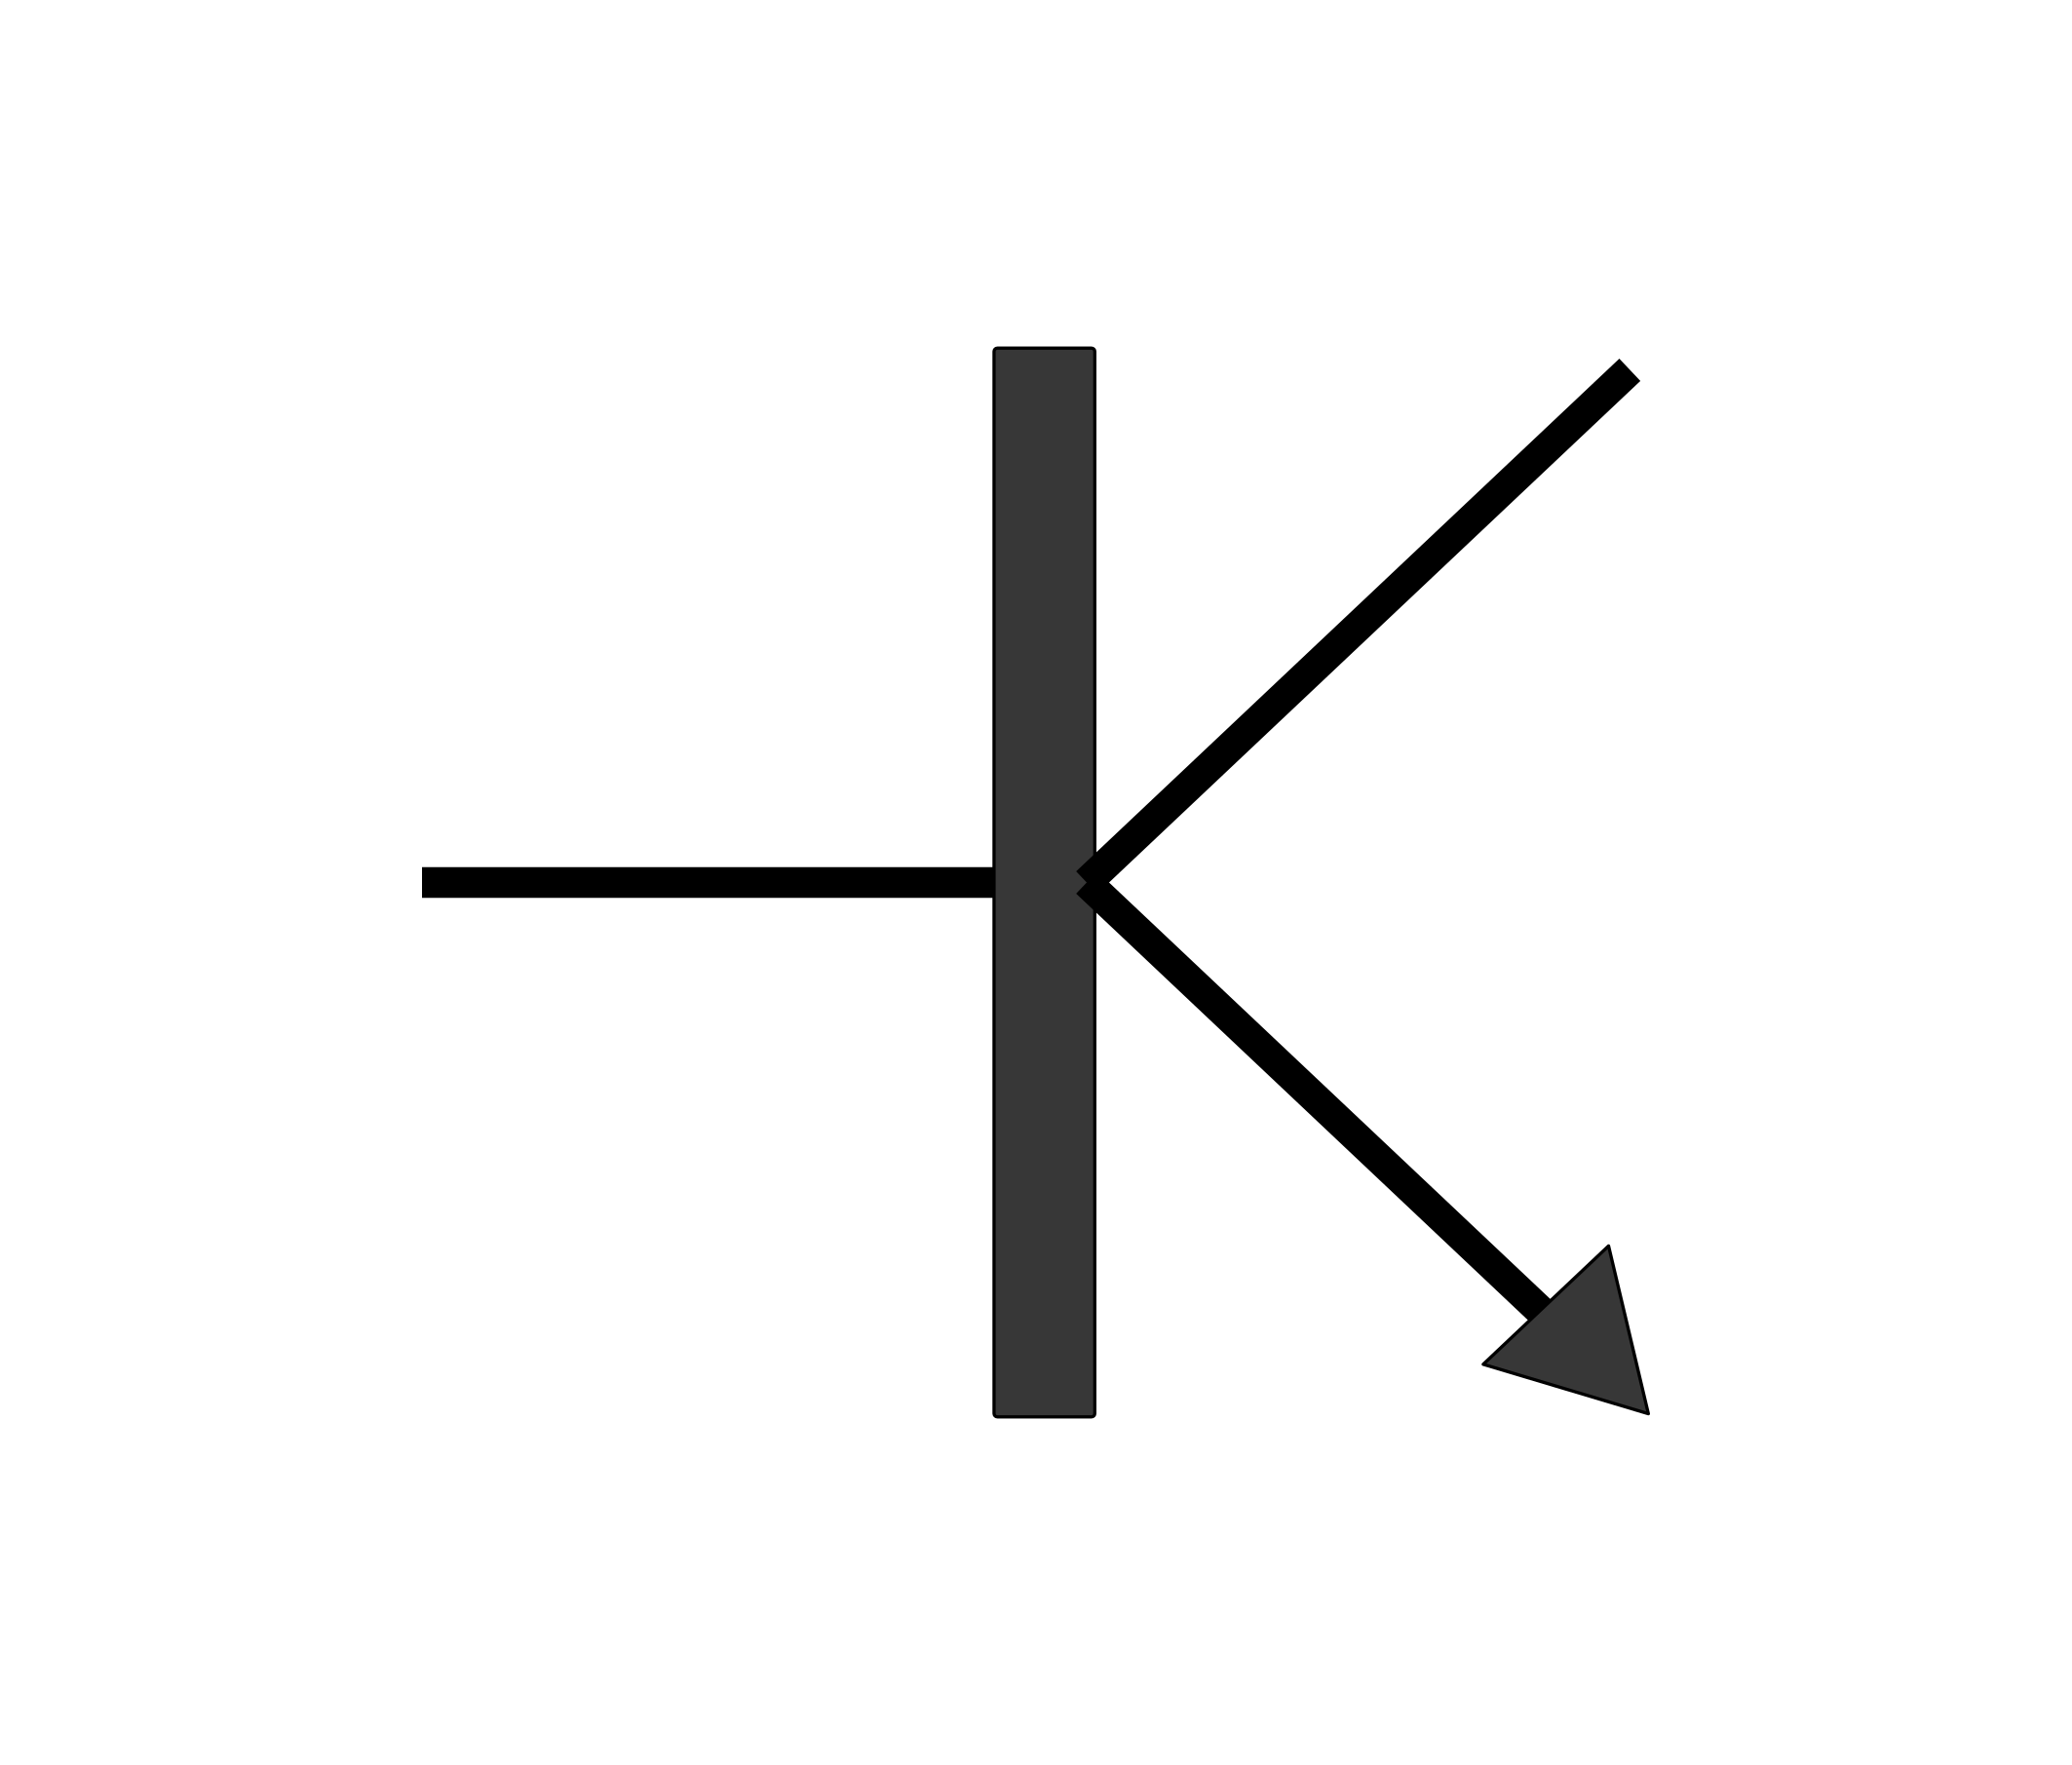
\includegraphics[width=0.5\textwidth]{bjt}

Then there are \gls{vltg} controlled switches, the main example of this being MOSFETs. Current can flow after the \gls{vltg} is higher than a threshold is reached in its gate. They are more complex to use, since the gate acts as a capacitor, so has to be charged, so may not function well without a properly considered gate charge circuit. Losses are related to the MOSFET's internal resistance, which can get very low, so they are typically fairly efficient.

\includegraphics[width=0.5\textwidth]{mosfet}

There are other switches, mainly for high power electronics, which don't require as much depth.

Relays are an alternate form of switch, which uses an electromagnet to cause a switch to open or close. Most switches work with DC, where relays are useful for AC applications. They are another form of switch that provides electrical isolation between parts, as it is an electromagnet which pushes the switch closed.

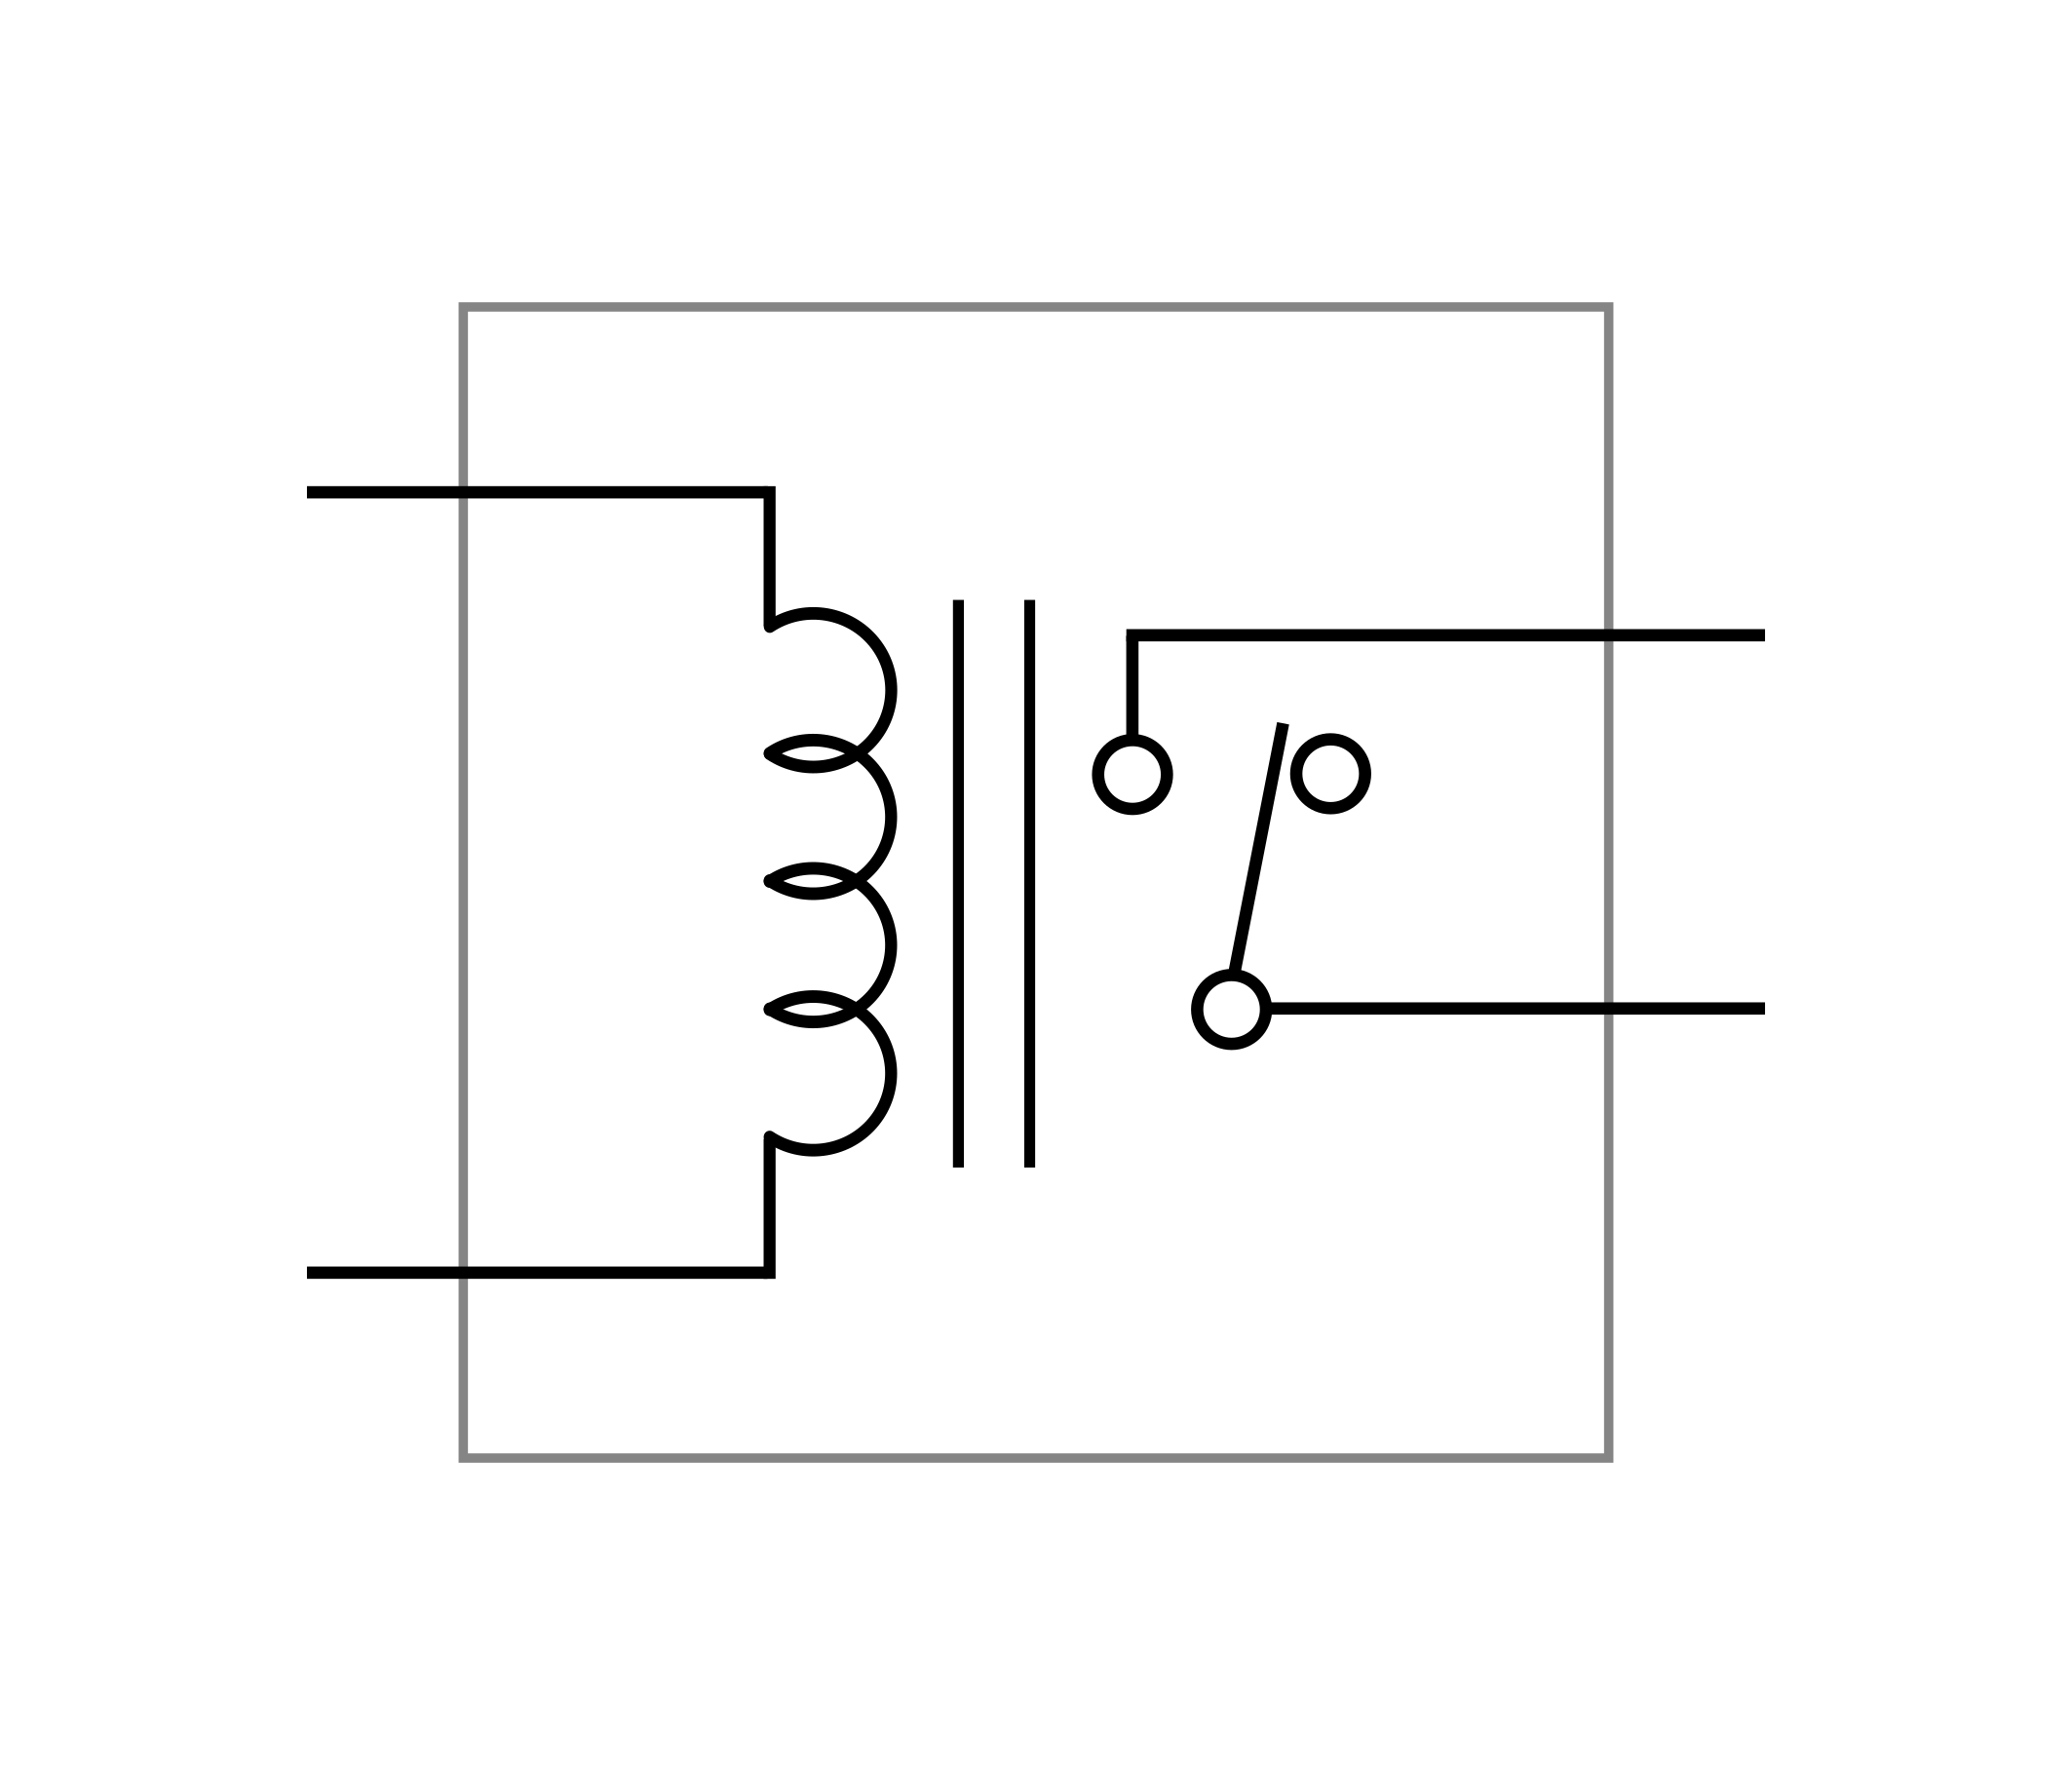
\includegraphics[width=0.5\textwidth]{relay}

Darlington transistors are also commonly known as a Darlington Pair, made of a couple BJT transistors, allowing higher levels of current amplification/ high current gain.

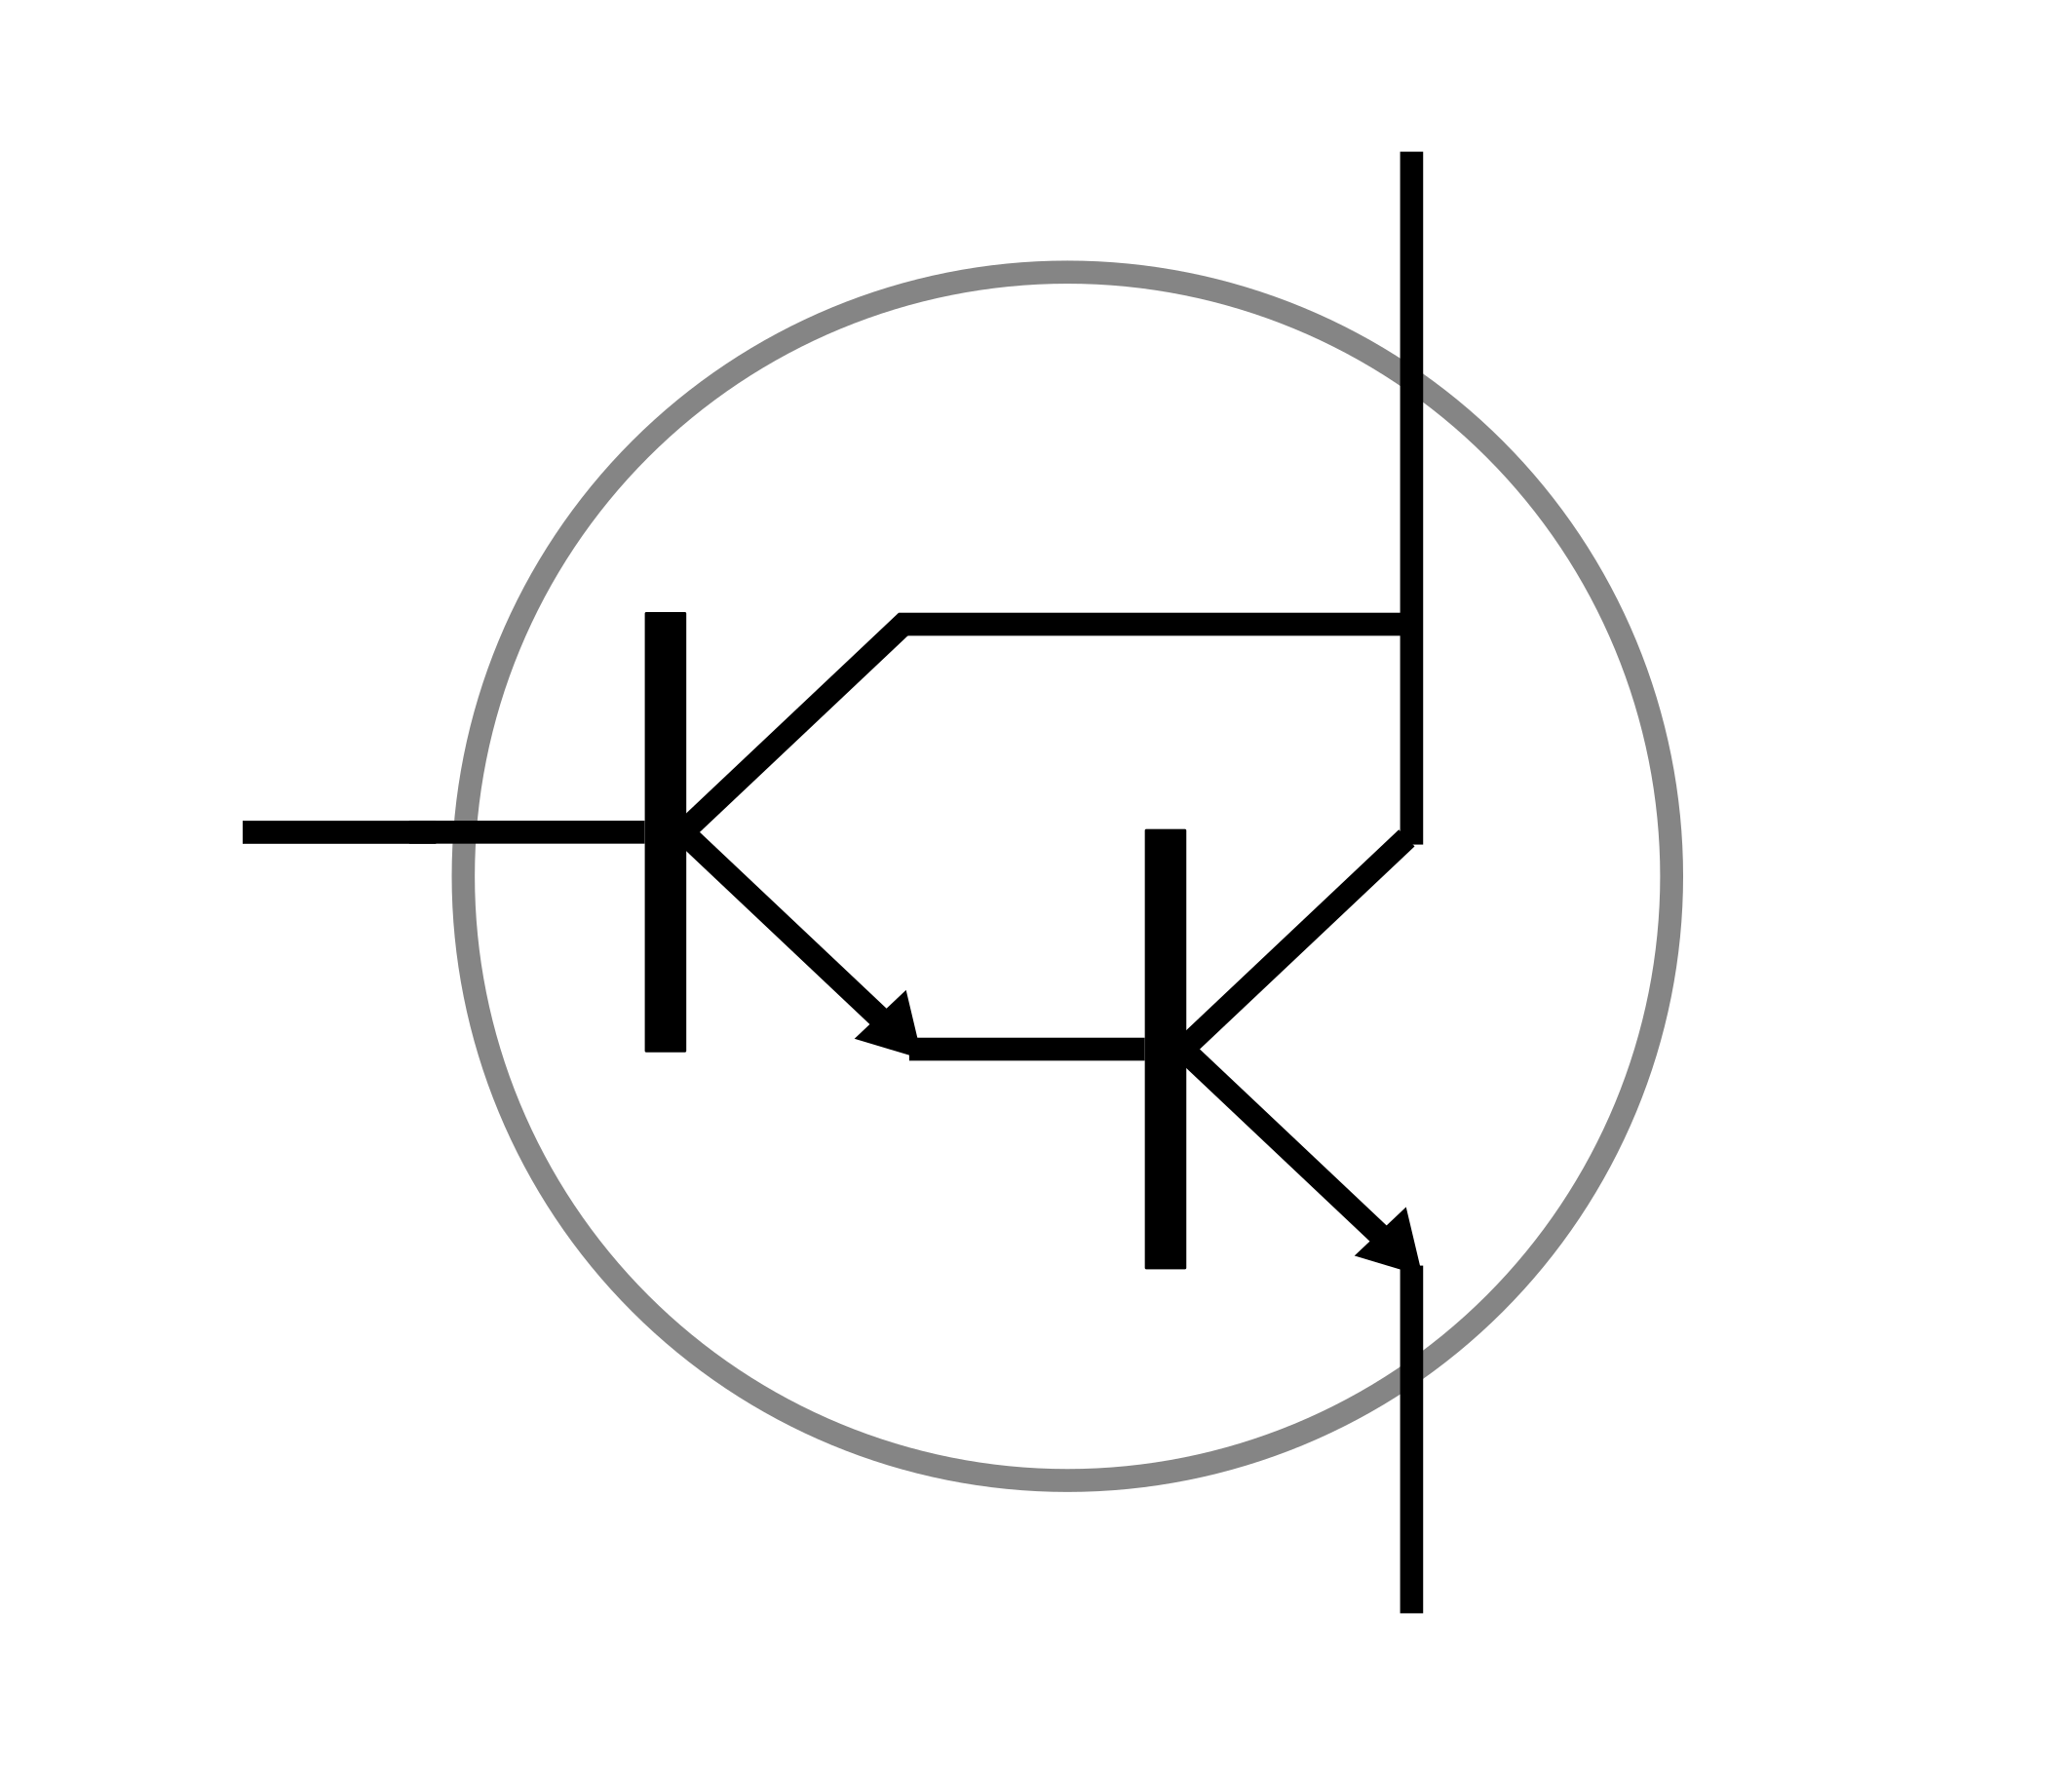
\includegraphics[width=0.5\textwidth]{darlingtontransistor}

You can get arrays of transistors, such as Darlington Arrays, which is a chip with multiple Darlington transistors with common emitters. These are useful for high power or inductive loads being controlled by a microcontroller.

\Quiz{Quiz}

1. What type of digital switch could you use for turning an AC motor on and off?

2. If you needed a simple transistor circuit to turn a high power LED on and off from a microcontroller, what type of transistor would you use and why?

3. What is the purpose of a transistor gate? Feel free to use an analogy to help you explain?

\subsection{Opto-isolators}

Opto-isolators, otherwise known as optocouplers, are components that use light to transfer electrical signals between two isolated circuits. This is important if the two circuits need differing \gls{vltg}s, or need isolating.

They use an LED and a photo-\gls{snsr}/ photo-transistor, so it is light that transmits the signals, which keeps them electrically isolated. They are useful for measuring AC using DC electronics, so have uses within AC-DC power conversion/ supplies.

It may be worth reading the sections on photo-\gls{snsr}s/ photo-transistors within \gls{snsr}s, as well as transistors and diodes, to fully understand this.

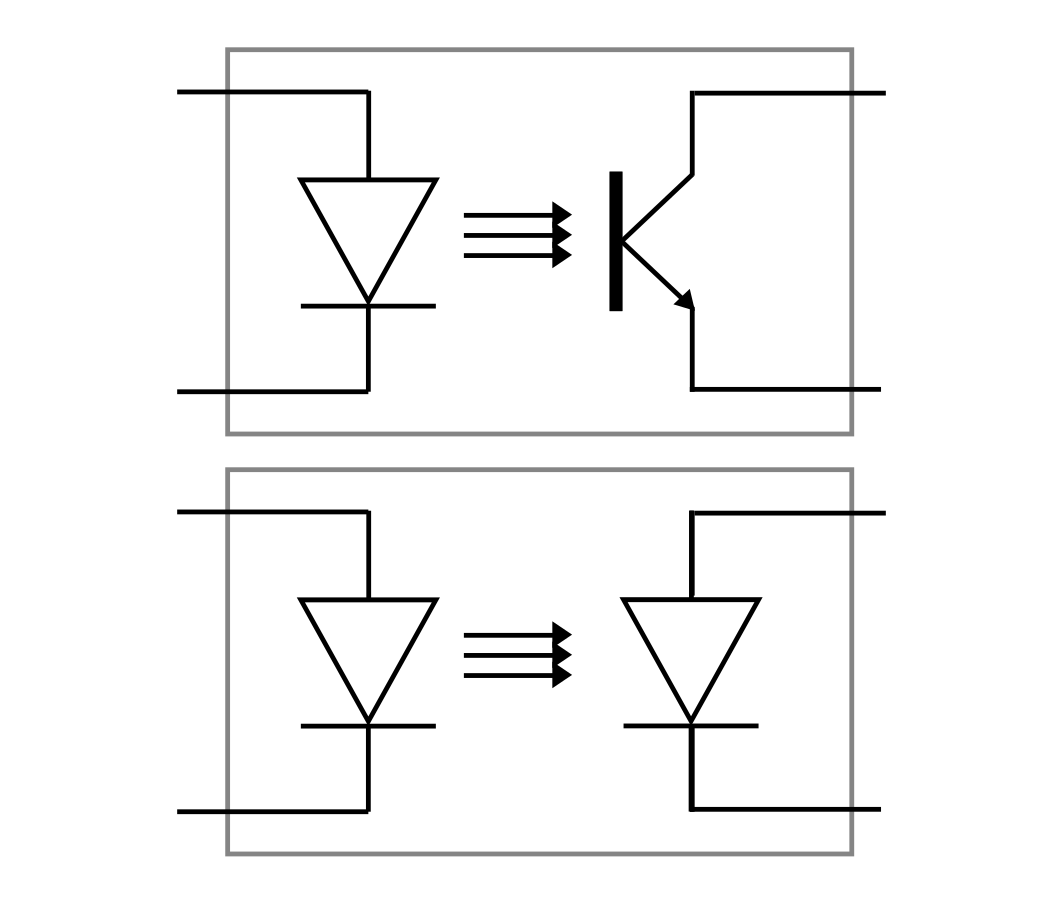
\includegraphics[width=0.5\textwidth]{optoisolator1}

\Quiz{Quiz}

1. Name an application where an opto-isolator would be helpful?

2. What components are within an opto-isolator?

3. Are opto-isolators suitable for transferring a lot of power?

\subsection{Power Sources}

It is important to consider what power source you should use for a given project.

Batteries come in many different types, some being rechargeable chemistries and others not. Many batteries use lithium, a very common material for rechargeable batteries, although it requires careful consideration and the use of a charge IC, to ensure that both its environmental and operating conditions are suitable. If not used wisely, it can be a dangerous chemistry with a range of risks stemming from mishandeling, shorts, over and undercharging and more.

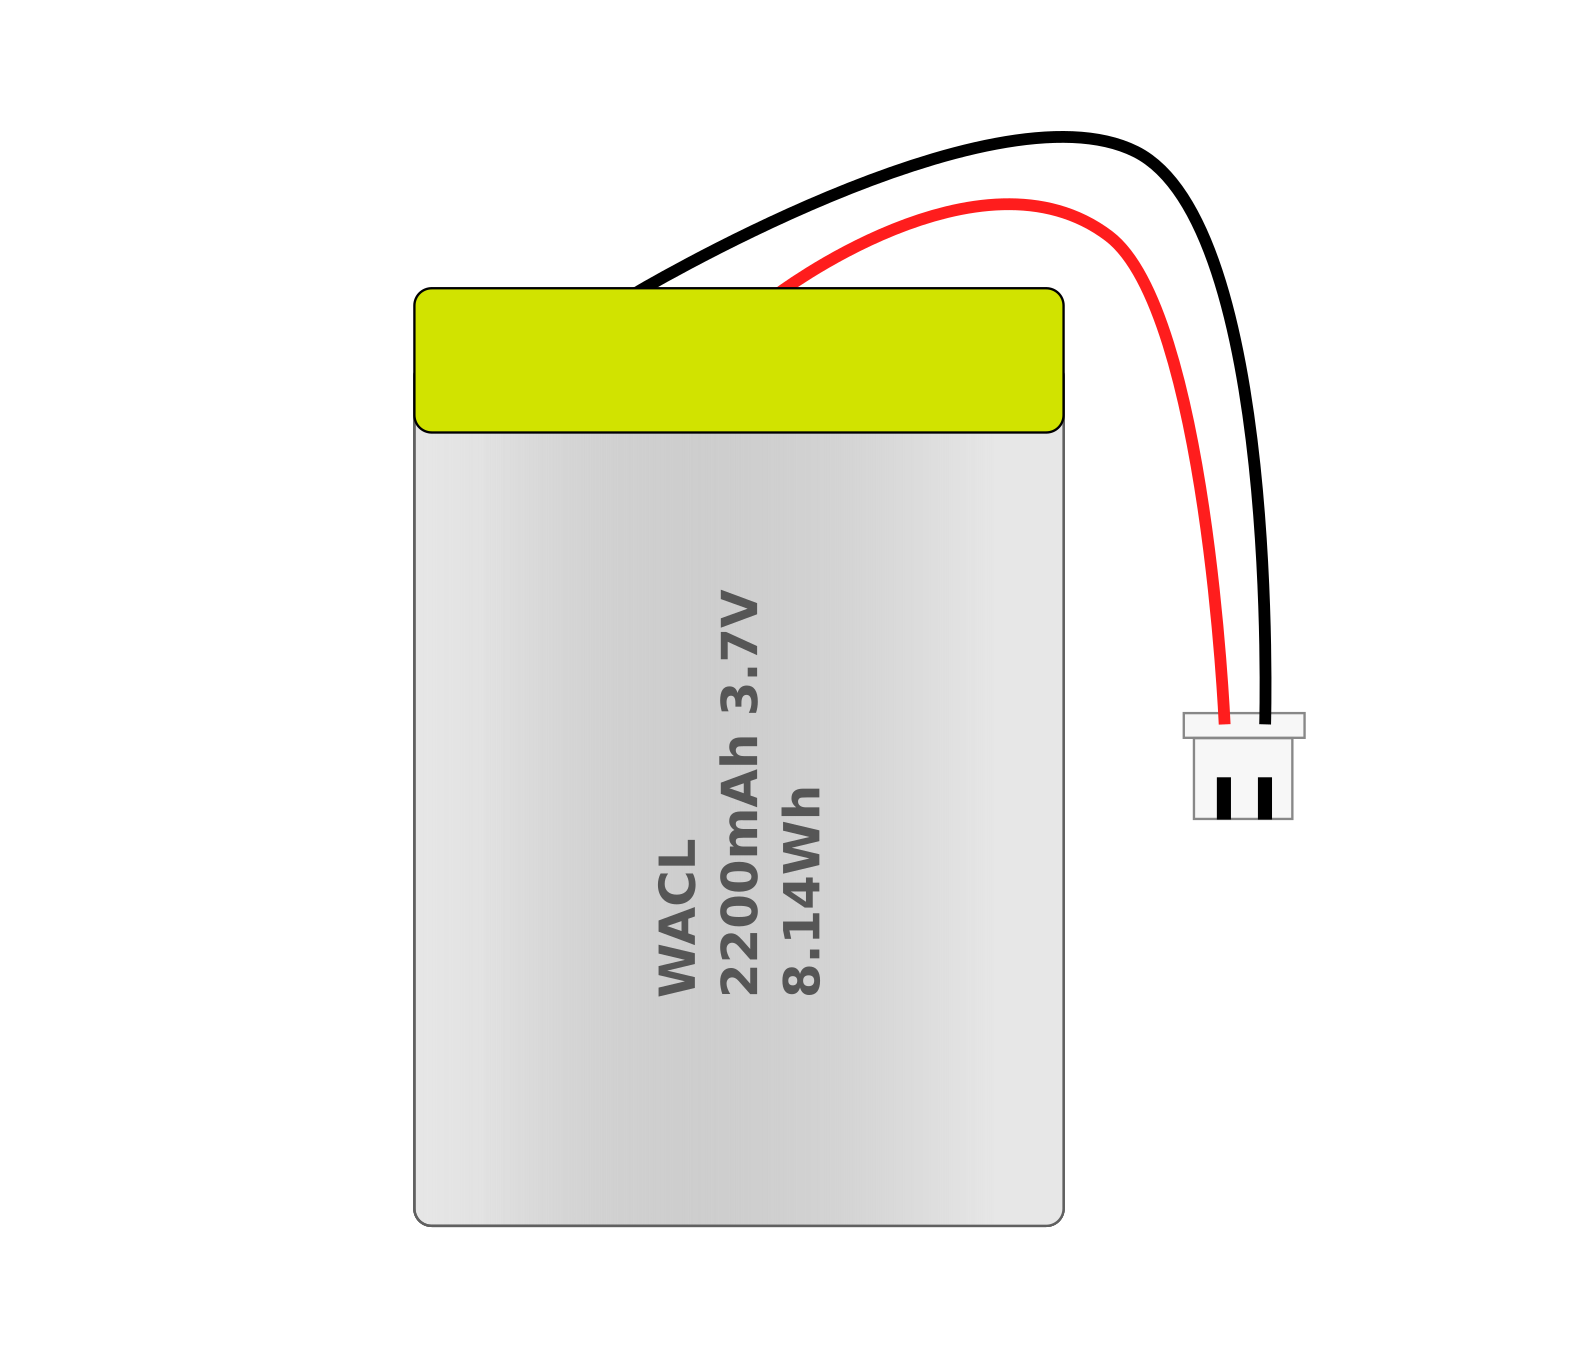
\includegraphics[width=0.5\textwidth]{lipobattery}

There are a few more forgiving rechargeable battery chemistries, one of the main ones being NiMH, which has characteristics in a similar magnitude to lithium cells, although generally worse in both energy and power density. Energy density is the amount of energy it can store either per litre or kg, so will affect how long a product will last, where power density is the magnitude of power it can continuously supply, again either per litre or kg. Energy density is given in Wh, which is the number of watts of energy it could supply for an hour.

NiCD and Lead Acid are two other battery chemistries which still get some use, but are decreasing in relevance due to them having worse characteristics in a range of aspects, and poor carbon footprint. Lead acid is still used for certain applications due to how easy it is to charge and discharge, and its low cost per Wh.

Along with battery sources, considering wired methods are also useful. USB is one of the more common methods, with most USB methods transmitting 5V. USB C for example allows for devices to "negotiate" their \gls{vltg} draw, between 5-20V, with a 5V default. Micro USB B, which used to be a standard for portable devices in some cases can handle a max of 3A, where USB C can handle up to 5A, making it suitable to power many projects. The connector has a higher durability, and can be inserted either way. Other data transfer can be done through it as well, making it versatile.

DC jacks are useful for power only, and can vary in dimensions and power output. It is fairly common to get DC jack based power supplies with 6V, 12V and 20V \gls{vltg} outputs, with a range of current outputs.

Adjustable DC power supplies are helpful for testing stages, or if specific \gls{vltg}s are needed, and will power a device with \gls{vltg}s between around 0-30V and sometimes 0-60V or more. 5A and 10A are both fairly common for max current output capabilities.

\subsection{Ideal vs Non-ideal Components}

Until now, we have talked about components as if they are ideal. This means they have no losses other than expected. In reality, components have internal resistance, capacitance and inductance. For low-speed circuit design, the internal resistance is what you mainly need to be aware of. This includes the source, with certain batteries/ sources having a high internal resistance, which means at higher current draws, there can be a fairly significant \gls{vltg} drop before it even gets to the rest of the circuit. Any of these factors can have a significant effect upon a more high-speed circuit, with capacitance and inductance altering over different frequencies. In high speed circuit boards, there are a range of techniques used to limit the potential for unwanted capacitance and inductance to affect a circuit. Issues such as this could be what causes circuit problems, especially for breadboard designs.

A battery/ power source would usually have an ESR value, which stands for equivalent series resistance. This is important to consider what losses, heat build up and \gls{vltg} drop could be seen at particular loads.

\section{Power conversion}

Power conversion could be its own course, so this lightly touches upon conversion for a base understanding and why it is important. Within the further reading section, there is information on rectification, combining theory above, so is worth checking for more of a challenge, or if AC-DC conversion knowledge is necessary.

The main types of power conversion are active and linear. Active utilises both capacitors and inductors, as well as switches for efficient conversion of \gls{vltg}, either to a higher or lower level, with efficiencies into the 90\% possible. Whereas linear power conversion is cheaper, requires a lower number of components and is specifically for decreasing the \gls{vltg} at the output. It acts as a variable resistor, to dissipate the unwanted \gls{vltg} as heat, so depending on the circuit's needs, can be particularly inefficient. Therefore, if efficiency is less important than costs, or the \gls{vltg} decrease is only very minimal, linear \gls{vltg} converters can be an okay option. Given how easy it is to find power conversion modules (either known as step-up or step-down, whether \gls{vltg} is increased or decreased), these are usually better than custom designs, as usually only a potentiometer needs altering to get necessary output \gls{vltg}, with minimal losses.

For a quick active power converter insight, a switch is turned on at set ratios to charge an inductor, which then discharges to charge a capacitor for a smoothed \gls{vltg} at the intended level. The ratio between the switch on and off times will affect the output \gls{vltg}.

The above mainly discussed DC to DC power conversion. To do AC to AC, a transformer is commonly used. AC to DC may use a similar method to the above but using a transformer rather than an inductor, and the use of a rectifier to convert the AC to DC.

\Quiz{Quiz}

1. Name three other types of conversion if the example is DC to DC.

2. True or false, active power conversion is always more efficient than linear power conversion?

3. True or false, it is typically recommended to use a module for active power conversion due to their design complexity?

\section{Communication Protocols}

\subsection{Wired Communication Protocols}

Communication protocols are important to interface with different devices and equipment, so a base understanding of some of the major ones would be important.

Communication protocols are a set of rules which devices follow to transfer information, allowing coherent data transfer at set speeds, depending on the use case.

It will first be useful to distinguish between serial and parallel, since these are widely referenced regarding communication protocols.

Serial means that there is a single data line/ wire used for communication in a given direction, where parallel means that there are several data lines or wires with data travelling through. Therefore, serial is often an easier method to use or implement.

They can first be split into two main kinds, with inter system protocols being those used to have communication between devices, where intra system communication protocols are meant for between component communication.

Therefore, you may use a combination of the two, depending on the project.

It is useful to know the term Port. Ports are points where communication can be done from, to a specific device.

USB and UART are the main examples of inter system protocols, where SPI, I2C and CAN are some of the main intra system protocols. Although some of the main protocols, it is not a definitive list, with niche or proprietary protocols being around. These may have specific benefits, or are proprietary to limit use of other companies' chips for a given application.

Master and Slave are still common terms within communication protocols, that you need to be aware of, although there is a shift to alternate terms such as controller and responder, although not yet standardised. Other alternatives could include primary and secondary, leader and follower and source and sink, although the latter of which already is widely used within electronics. Because of the negative connotations of master and slave, this course uses the suggested terms of controller and responder.

USB is very widely used and is how many devices are connected to computers. It is high speed, and quite simple to implement, although requires the use of specific drivers and a powerful controller. USB 1 and 2 have 4 pins, one for power, one for ground and two for data, with data being sent serially in each direction.

UART is physical circuitry for conversion between serial and parallel data, where two UARTs may communicate with each other, communicating in serial, meaning that only two wires/ data lines are necessary for communication between two devices.

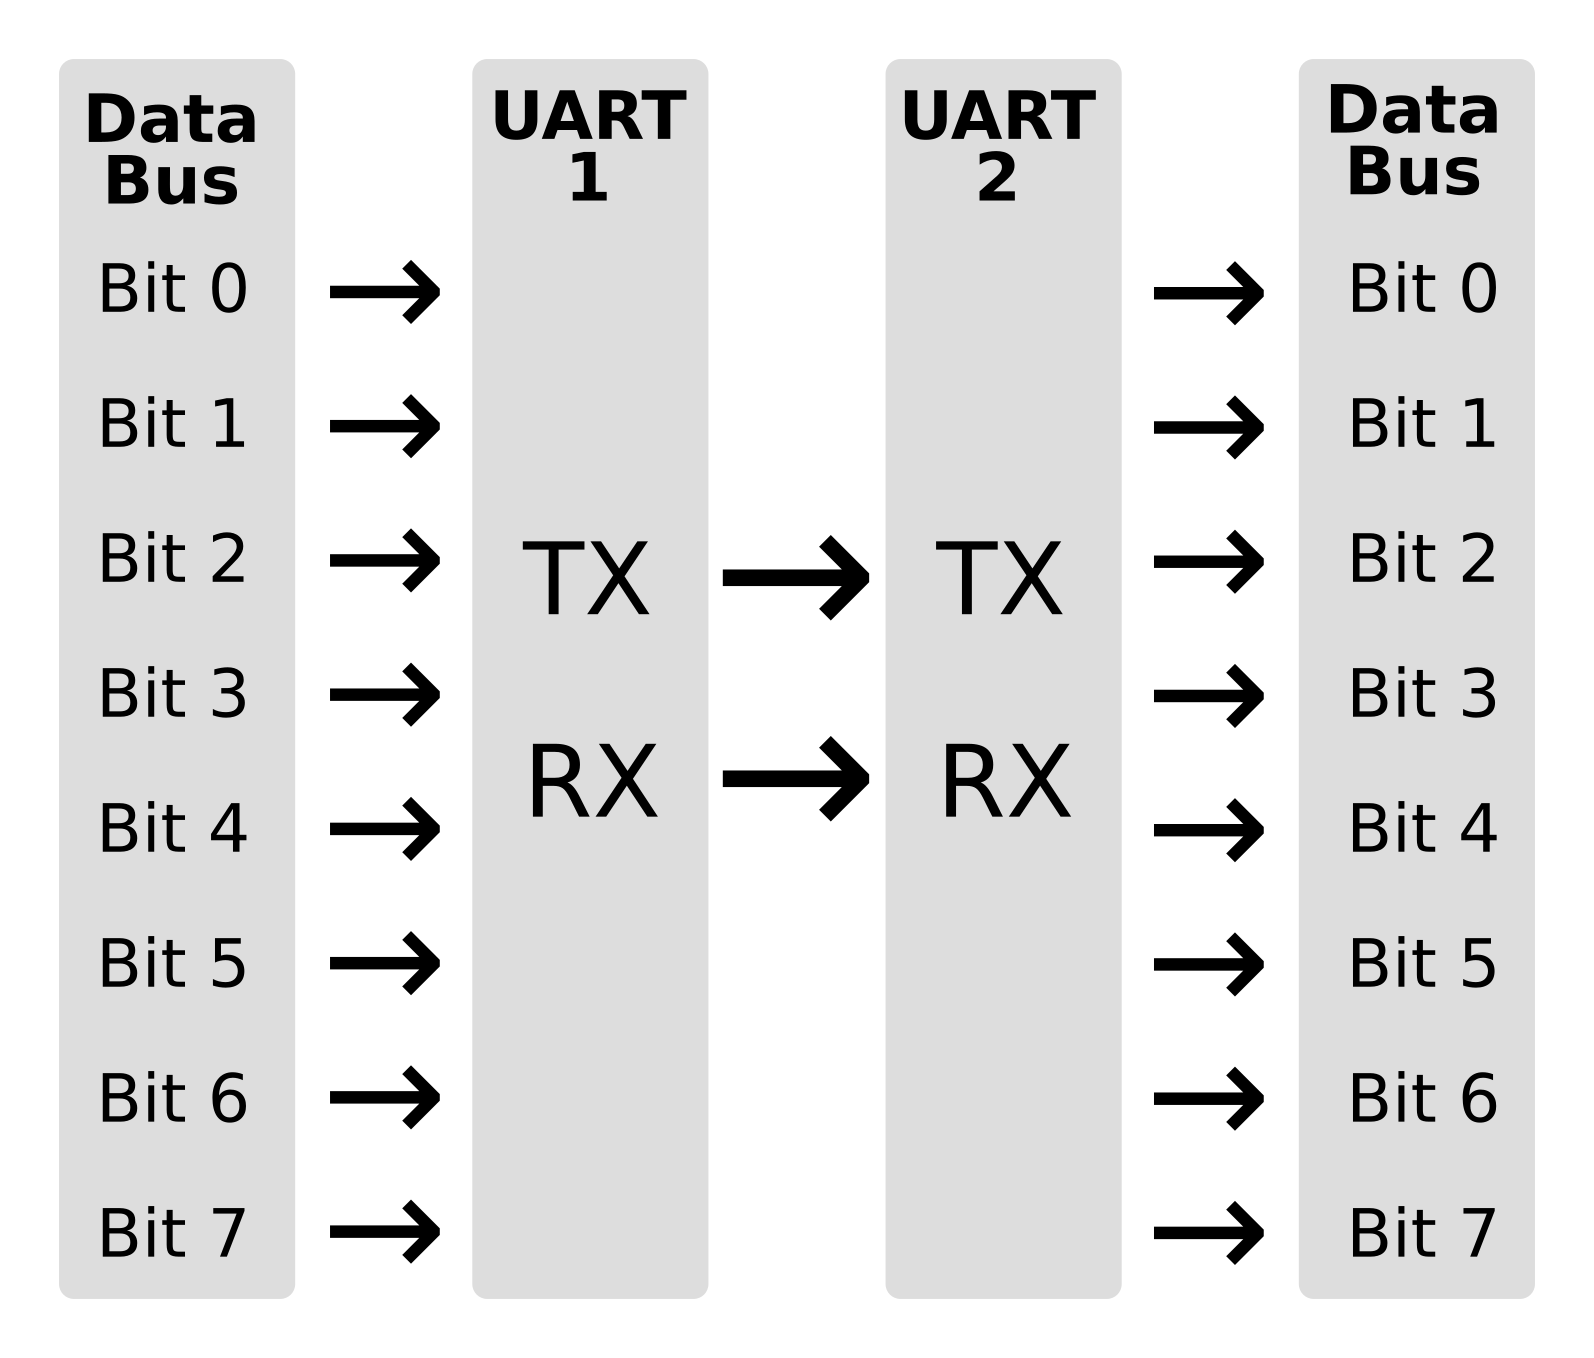
\includegraphics[width=0.5\textwidth]{UART}

RS232 is another protocol (Recommended standard 232), which is often used within telecommunications. In general, it is often used for connecting devices such as data acquisition or modems, the prior of which are likely to be particularly important. On creation, RS232 allowed for "handshaking", a method for checking that data is transmitting correctly, although many devices no longer require the use of this. RS232 can directly connect to the serial port of a computer.

ModBus is a protocol which was created for communication for programmable logic controllers, often for industrial use. One reason for its wide usage is that it has no royalties and is open.

SPI is a commonly used protocol, which has a single controller and multiple responders connected to it. SPI stands for Serial Peripheral Interface, with there being 4 main lines used, two pins for data transfer, a pin for selecting which responder the controller is communicating with and a line used as a clock. Therefore, for each responder that the controller wants to communicate with, a separate select pin is required. It is a relatively fast communication protocol, but doesn't scale the best due to needing a new GPIO pin for each new device.

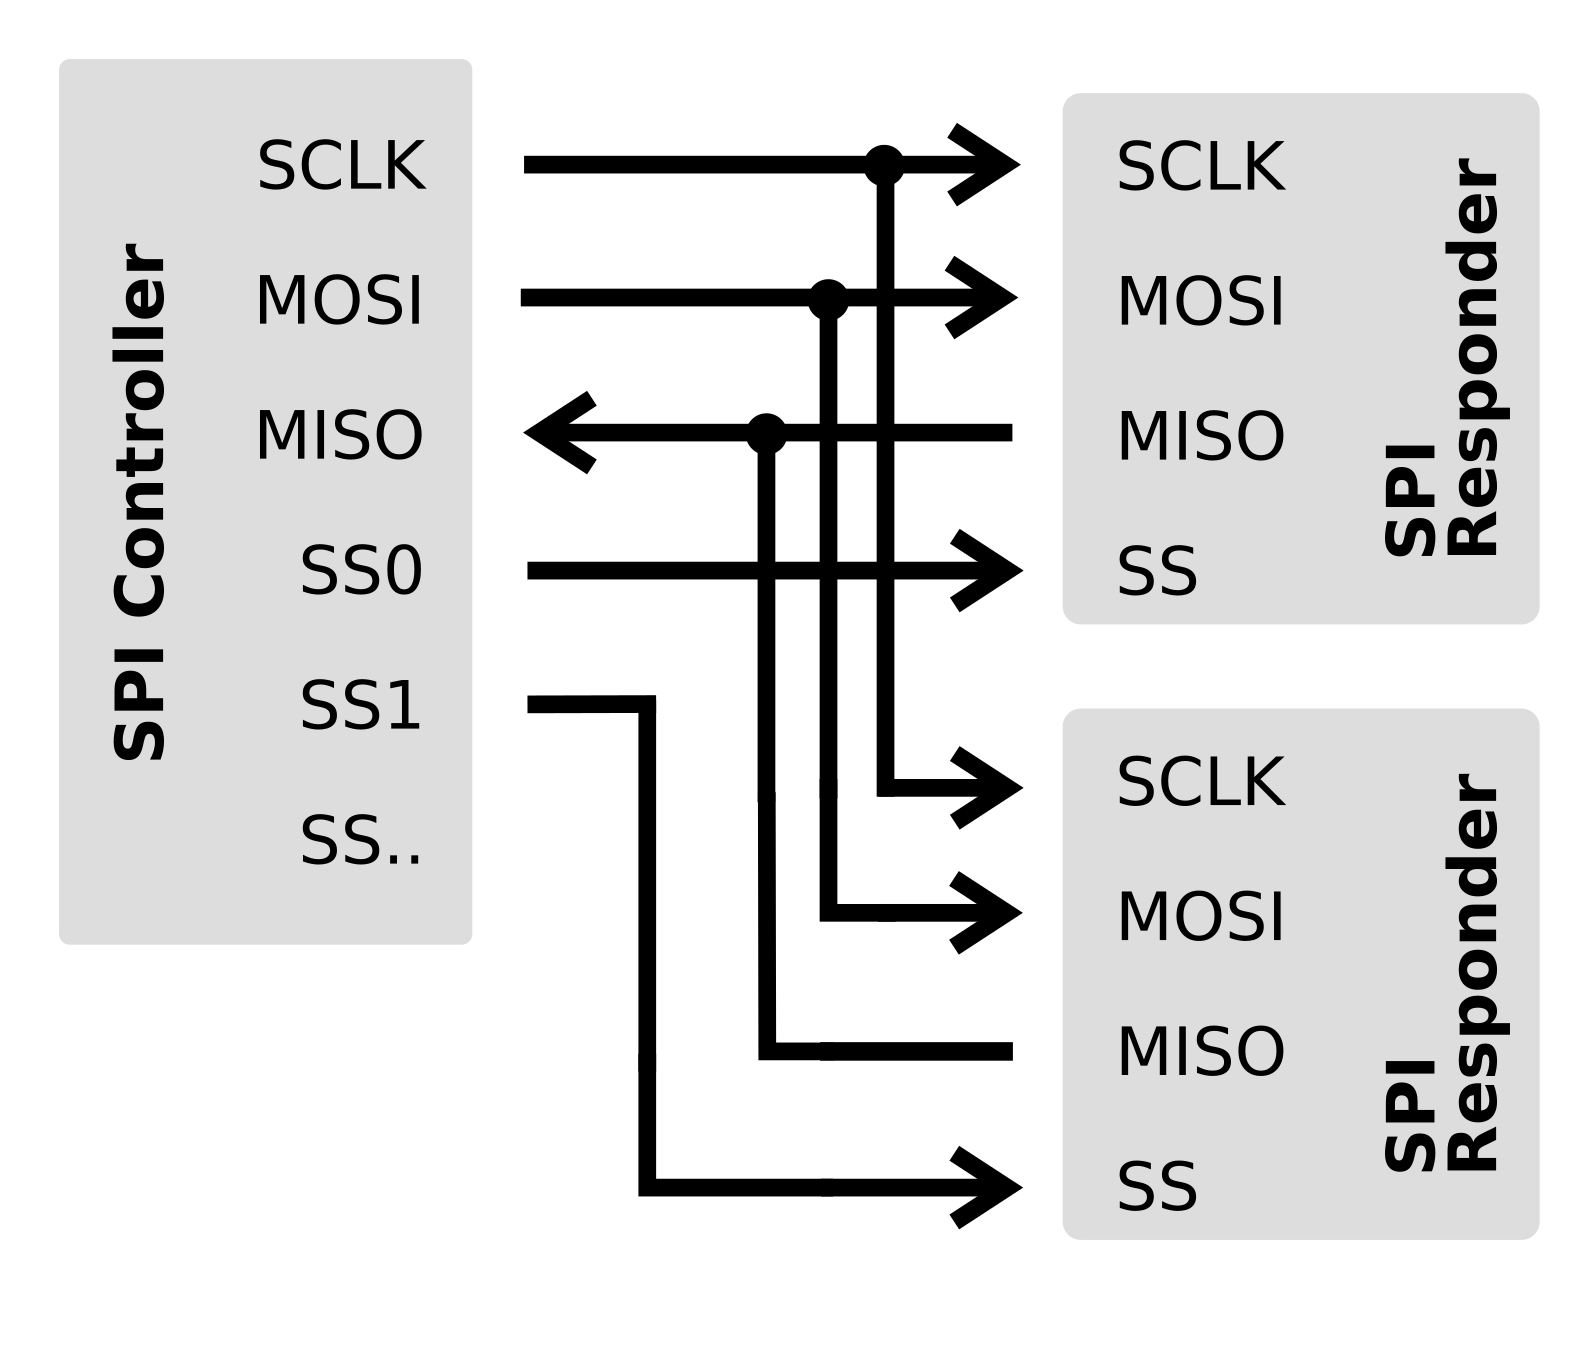
\includegraphics[width=0.5\textwidth]{SPI}

I2C is a similar protocol, which is also synchronous, like SPI, controlled with a clock from the controller. It only requires two wires for communication, the clock and the serial data line. It can communicate with many devices/ responders with just two wires, but is limited in speed and has a combined transmitting and receiving data line.

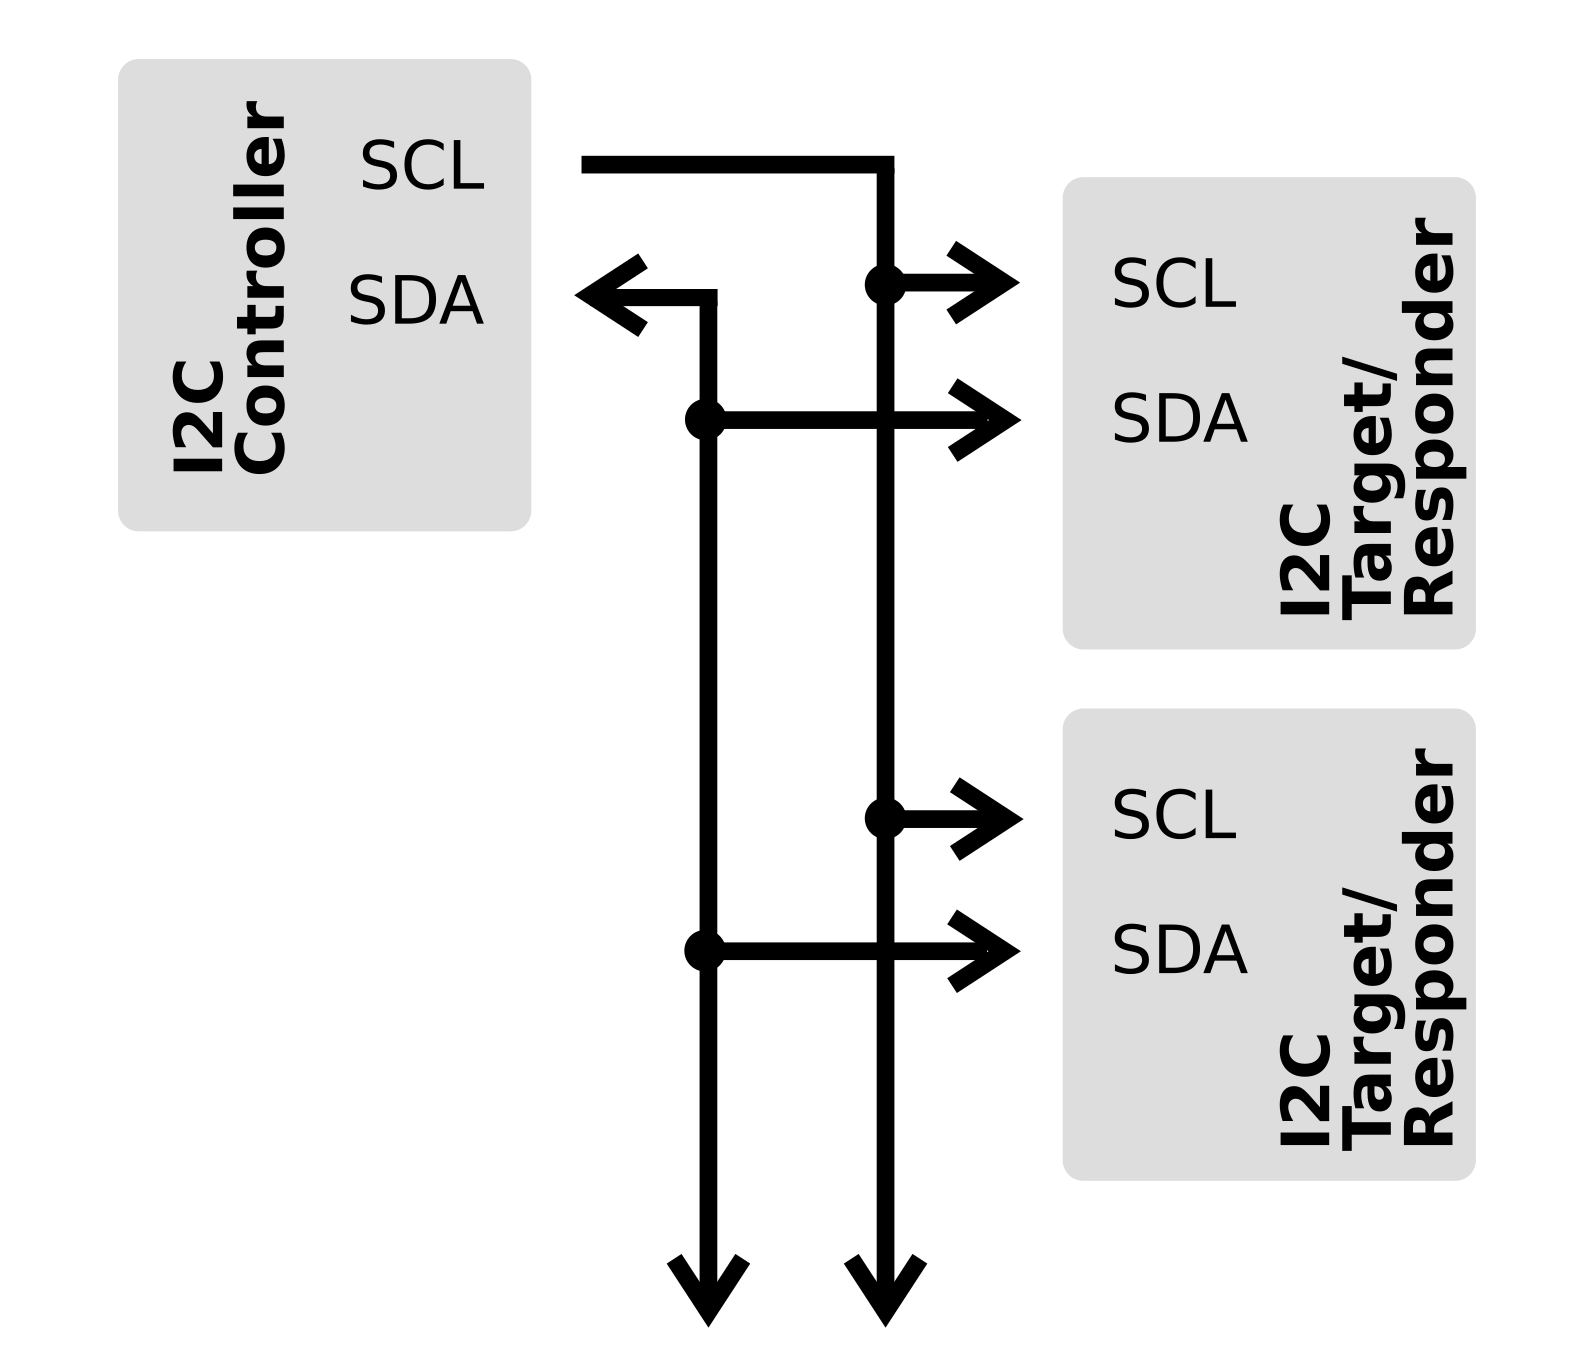
\includegraphics[width=0.5\textwidth]{I2C}

CAN stands for Controlled Area Network, and is a protocol meant for the transmission and receipt of data within a network of devices, especially for harsher environments. Due to this, it is mainly used in industrial and automotive environments, so may be used by certain research equipment. It is fast, secure and low cost, but is complex and automotive orientated.

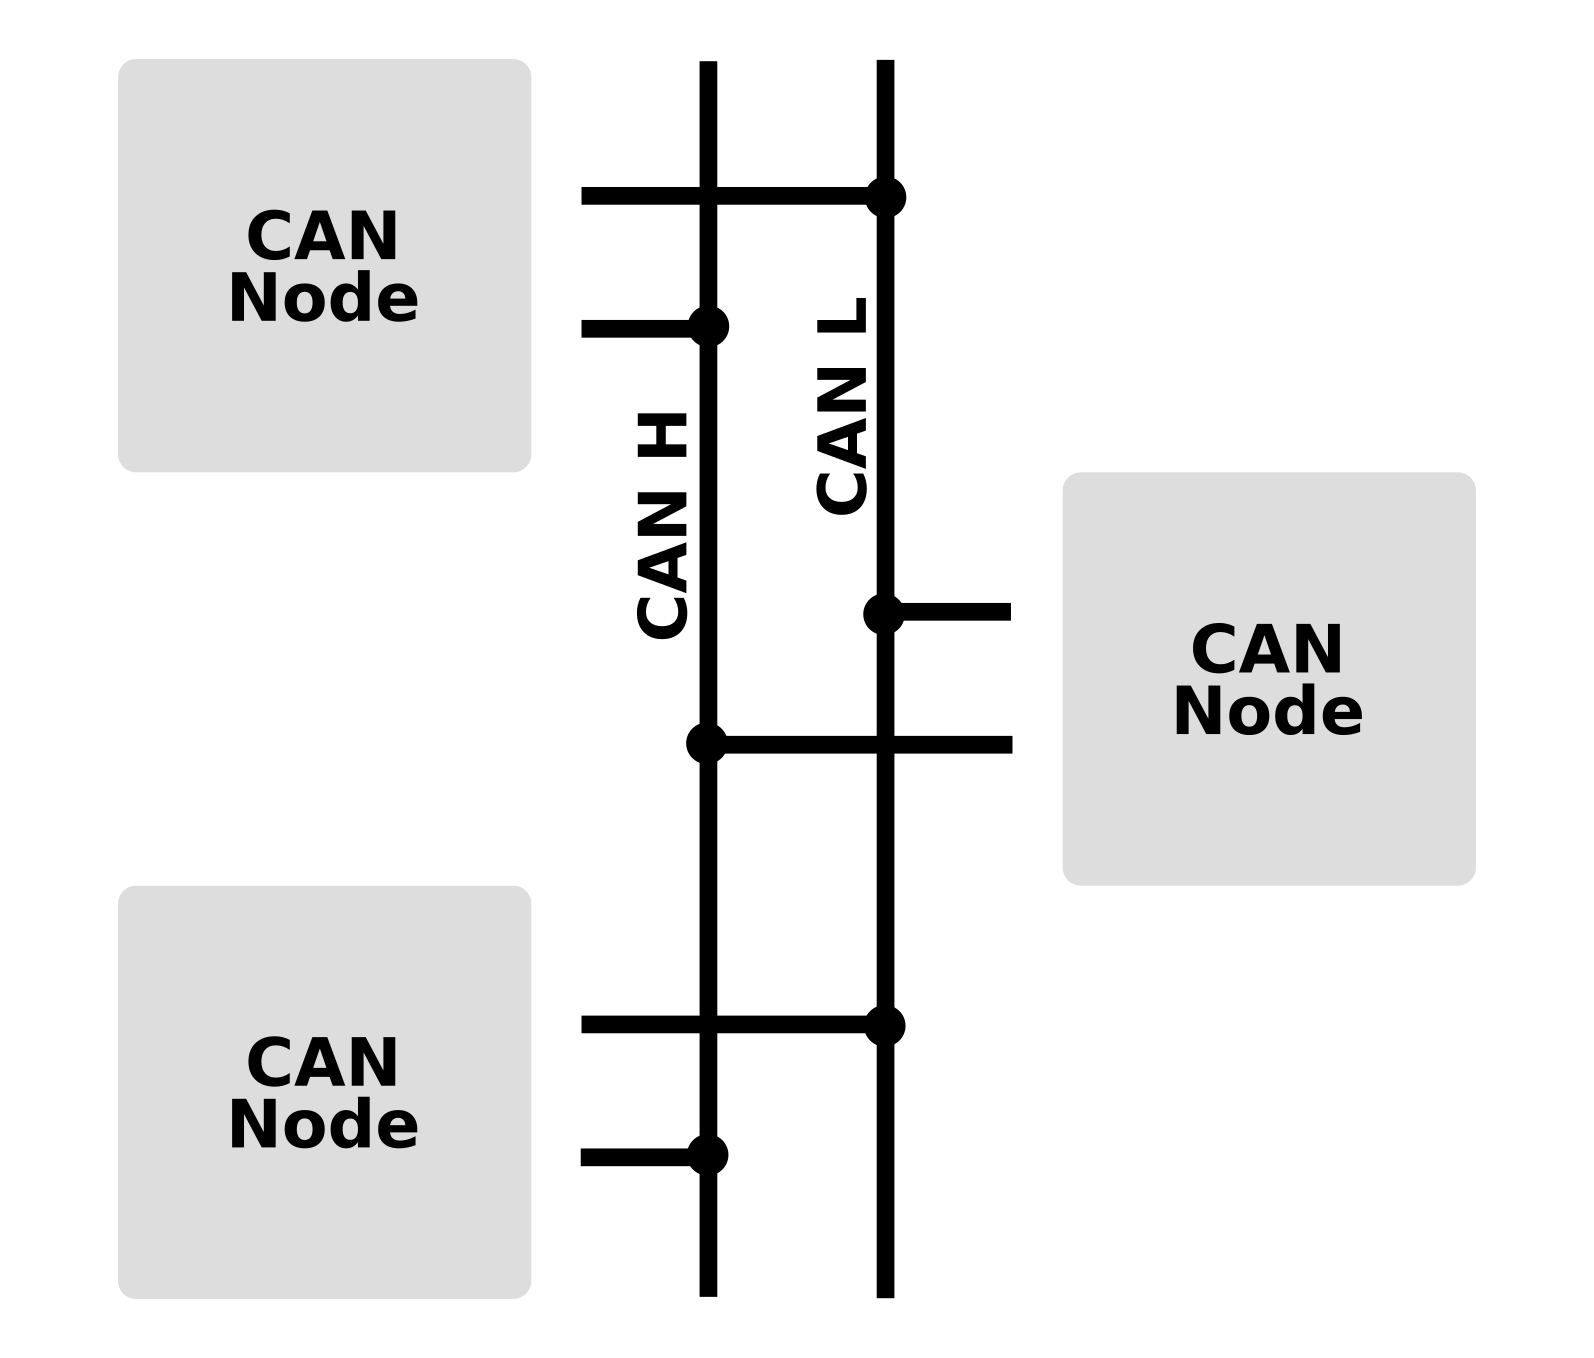
\includegraphics[width=0.5\textwidth]{CAN}

Since not all devices have protocols that are usable together, there are chips for conversion of protocols, often seen as modules which are often used to interface between a device and a computer. As previously mentioned, USB often requires drivers to be installed, so you should be aware that you may need to download a driver for interfacing with it.

This section will quickly go over modules/ chips you may come across for communication with these different protocols.

USB to UART modules are very common, often having a USB port on one side and 4 pins on the other. These may use a range of chips and are likely to use TTL level, which is transistor-transistor logic between the limits of 0 and VCC, which is often either 3.3V or 5V. A supplier will mention whether it works at TTL \gls{vltg}s, or others such as RS-232, a standard meant for telecommunications.

\subsection{Wireless Communication Protocols}

Although we won't go into too much detail, it is helpful to be aware of some wireless communication protocols and their benefits.

Wi-Fi- This is a family of wireless protocols meant for local area networking, and is one of the most widely used.

Bluetooth- Bluetooth is a short range communication protocol, meant for communication between a fixed and mobile device. It has been through several iterations, with Bluetooth 5.0 having distances upwards of 400m, but it is typically below 10m.

ZigBee- This is meant for creating local area networks of devices, with communication range between 10-100m.

LoRa- This is a long range radio protocol meant for unlicenced radio bands, with ranges in the Km range being viable, depending on the landscape and antenna used.

GPRS- This is the protocol which is the mobile standard for 2G and 3G mobile networks.

\section{Integrated Circuits (ICs) and Microcontrollers}

Along with the discrete components mentioned above, there are many integrated circuits, components with a circuit built in for specific functions. A complex example of this, which is widely used, is microcontrollers.

Integrated circuits may do a wide range of things, such as amplification, timing and power conversion. These help to decrease the time, complexity, power consumption and often costs of a design by packaging all the discrete components necessary for its function. Usually a few passives or discrete components are required, which are referenced in the parts datasheet.

This section will quickly talk through some of the more important integrated circuits and their uses.

Amplifiers- A range of chips meant for the amplification of signals, usually analog signals.

Circuit Protection- A range of components meant to protect other aspects of the circuit, such as digital fuses or ESD protection.

Timing- A range of chips to provide the timing of other chips.

Data Conversion- Chips used to convert one type of communication protocol to another, or for analog-to-digital conversion.

Display/ LED Drivers- Chips meant for the driving of displays or LEDs.

Interface ICs- Chips meant for communication over different protocols, or to interface with different parts/ devices.

Communication ICs- A range of ICs and modules for wireless communication, such as Wi-Fi, Bluetooth, LoRa, ZigBee.

Logic ICs- Chips that work through low level boolean logic, for building logic based circuits.

Memory- Necessary for storing data.

Power Management- A range of chips for power management, whether this is active or linear power conversion, battery management, power monitoring or other driving chips.

\gls{snsr}s- A range of chips for interfacing with analog sensing elements or combining both into a single package.

\subsection{Microcontrollers}

Microcontrollers are low power processing units, with built in memory, that can be programmed to do a range of functions. These may typically be put together as a single complete unit, such as an Arduino board. An Arduino is a board with a microcontroller, passives and discrete components to interface with basic electronics components.

There are a range of protocols by which microcontrollers may communicate by. They also may contain a range of integrated circuits, to help interface it with different components, such as with an analogue \gls{snsr}. ADCs are frequently used (often internal to a microcontroller but are also available as an IC). An ADC is an analogue to digital converter, which will represent an analogue value as a bit value, depending on its resolution. This allows a \gls{vltg} reading to be associated with a digital value, for use within the program.

The pins of a microcontroller that enable data transfer are known as GPIO (General Purpose Input Output) pins. This term is widely used, but sometimes may just be written as IO pins. These have limitations, such as what protocols they can be used for, along with electrical limitations like max \gls{vltg} tolerance, or current output.

These have a built in processor, which operates at a set clock speed, as well as RAM, ROM and sometimes FLASH memory. A processor is what computes instructions, based on what is in memory. These operate at a set rate given in Hz, with some instructions possibly taking multiple cycles. They are commonly in the MHz region. RAM is fast access memory, to store data which is needed by the program, such as variables. Then memory such as FLASH is slower access, used for storage of whole programs, which elements of which can be moved into RAM when it needs to run.

\subsection{Amplifiers}

Amplifiers are there to increase the amplitude of an analogue signal, often useful for use alongside analogue \gls{snsr}s, to take it to a \gls{vltg} range readable by a microcontroller. A common component for amplification is an opamp, which, when wired differently, can amplify a \gls{vltg} difference, or amplify a signal by a specific amount. This can be negative or positive amplification.

An understanding of how amplifiers work internally is beyond the course scope, although understanding of their uses is helpful. We will touch upon the types mentioned above in some further detail. Each of the below uses an opamp as the principal component.

The primary focus will be on the use of opamps to create amplification circuits.

Although, not an amplifier, it is important to separate two circuit elements. This is known as a \gls{vltg} follower, which isolates the resistances at either end of the part, particularly important where you may try to read a resistance value from a \gls{snsr}.

\includegraphics[width=0.5\textwidth]{voltagefollower}

There are non-inverting and inverting amplifiers, which the first of which amplifies a \gls{vltg} in its current direction/ magnitude, and the latter amplifies a \gls{vltg} in the negative/ opposite direction or magnitude.

\includegraphics[width=0.5\textwidth]{noninvertingamp}

\includegraphics[width=0.5\textwidth]{invertingamp}

There are summing amplifiers which can add two \gls{vltg}s together.

\includegraphics[width=0.5\textwidth]{summingamp}

Differential amplifiers output the difference between two \gls{vltg} inputs, with a certain level of amplification.

\includegraphics[width=0.5\textwidth]{differentialamp}

\section{Boolean Logic}

Boolean algebra is a branch of mathematical algebra, where variables are true or false, and it is centred around three main operators "And", "Or" and "Not", and several sub-operators.

For this section, the practical elements use DDSIM, another online simulator, developed by a lecturer at the University. Although similar functionality can be done through Falstad circuit simulator, DDSIM is more streamlined and intuitive for digital/ boolean electronics. Feel free to see which you prefer for which task, as they are not completely different.
https://www-users.york.ac.uk/~dajp1/Temp/ddsim.html
(There is also DASIM, for analogue electronics, similar to Falstad, where it can be easier to draw up circuits, it isn't quite as easy to visualise, https://www-users.york.ac.uk/~dajp1/Temp/dasim.html).

First, we will describe what the different operations mean. Regard it as a comparison of usually two inputs, either true or false, on or off, a \gls{vltg} present or not, or 1 or 0. We will use true and false, being the main terminology in boolean algebra. First, "And", is where both inputs are true, the output will be true, with any other combination having a false output. Then there is "Or", which states if either or both input is true, then the output is true. The last key type is "Not", which has a single input, where the input is the reverse of the output, true-false, false-true. Within electronics/ circuitry, gates are used to allow this logic, so you have And gates, Or gates and Not gates. There are several more complex examples, such as NAnd and NOr, which are a combination of an And followed by a Not and an Or followed by a Not. Another more complex example is an Exclusive Or (XOr), which has an output which is only true if only one input is true. A combination of transistors can make these gates, with a combination of NAnd gates creating any gate. This has become the normal, since NAnd gates are simple to produce from transistors.

In the examples, we have used A and B as the inputs and O as output.

\includegraphics[width=0.5\textwidth]{andgate1}
\includegraphics[width=0.5\textwidth]{orgate1}
\includegraphics[width=0.5\textwidth]{notgate1}
\includegraphics[width=0.5\textwidth]{xorgate1}

Boolean logic has led to modern computing, as it is a combination of logical operations done with gates. There are fairly standard circuits you can try to make, to ensure you fully understand boolean logic.

A famous theorem within Boolean logic is De Morgan's Theorem/ Law, which shows how AND logic can be represented through OR. We will use the below to represent this-

A \& B are our inputs or "sets".

$\bar{A}$ is the compliment of A, equivalent to A through a Not gate.

$\cap$ is the intersection, otherwise known as an AND gate.

$\cup$ is union, otherwise known as an OR gate.

With the terminology explained, De Morgan's Law can be shown as the below:

$\overline{A\cup B} = \bar{A}\cap\bar{B}$

$\overline{A\cap B} = \bar{A}\cup\bar{B}$

This also helps to explain why NAND gates are typically used within circuitry to represent other gates.

If this is an area that particularly interests you, I would recommend looking at the site, \href{https://nandgame.com/}{Nandgame}, which takes you step by step from placing gates to building a basic gate computer.

\section{Electronics equipment}

There are a range of equipment that aids working with electronics, some may seem initially overwhelming. Understanding what they do, why and if they are needed, is important!

\subsection{Multimeters}

A very common piece of equipment is a multimeter. These are used to measure current, \gls{vltg}, and resistance. When measuring current, the multimeter needs connecting in series with what is being measured. In contrast, to measure \gls{vltg} or resistance, you place the probes in series with the component or circuit segment needing measuring.

There are analog and digital multimeters, the latter more common, and what this course focuses upon.

We will talk through the main multimeter functions now.

You can measure resistance, current, \gls{vltg} and continuity on most, with some measuring hFE or current gain of BJT transistors. Some may also measure capacitance.

Depending on the multimeter, some will split each of the sections into specific scales, representing the max value it can show. This is so the resolution shown is close to the measurement magnitude. If, when trying to measure a value, nothing seems to be read, you may need to alter this scale.

The continuity tester is used to check whether two points within a circuit are connected, or whether current can flow between them, so is helpful for checking soldering.

For most functions, connecting the cables to the V/\ohm/mA section would be suitable as well as COM/ ground, unless it is a high current circuit, if so there is the third connection usually for currents at a maximum of 5A or sometimes 10A.

A more complex piece of equipment for complex diagnosis is an oscilloscope. These are used for measuring \gls{vltg} and current, compared against time, in graphical format. The software sometimes used within this course Falstad, uses scopes which are a representation of what you would view through an oscilloscope probing a specific component or circuit element. They are particularly helpful for troubleshooting signals or inductors or capacitors.

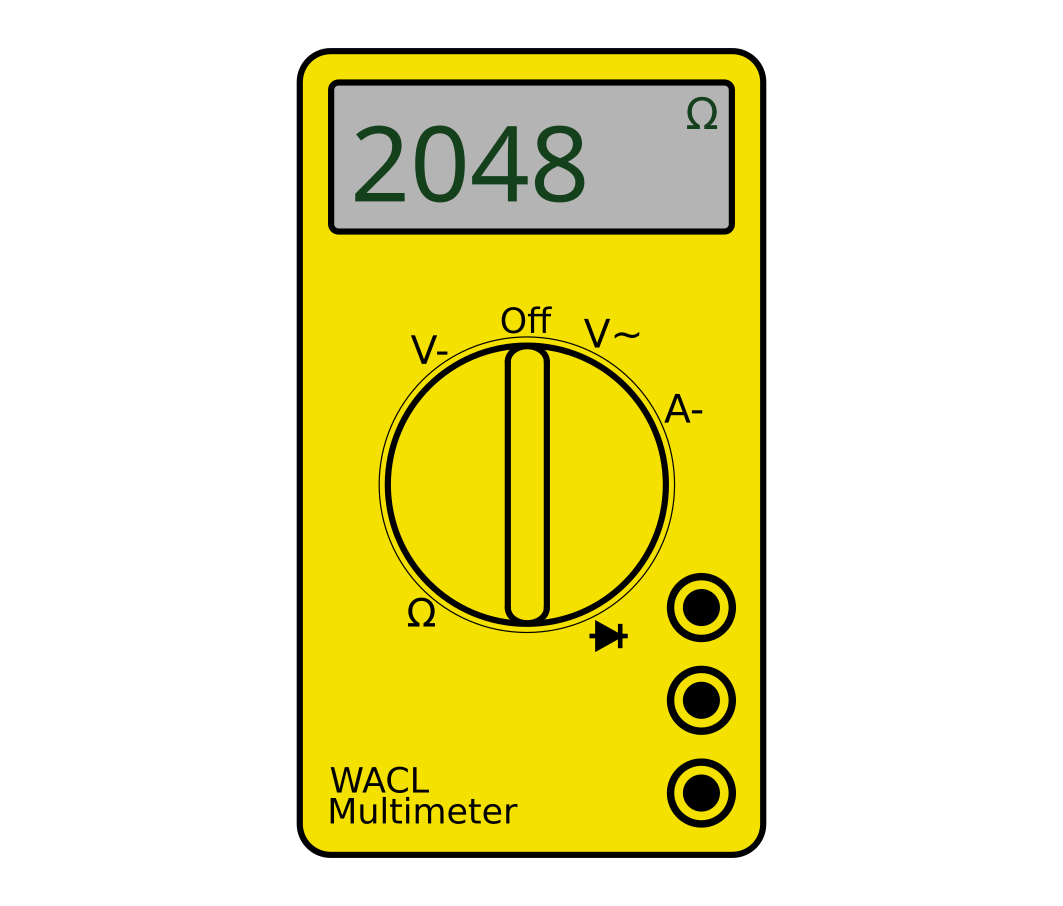
\includegraphics[width=0.5\textwidth]{multimeter1}

\subsection{Breadboards}

For electronics prototyping, breadboards are seen to be important, as they allow you to connect DIP components quickly for prototyping. They have many rows of 5 pins which are interconnected, so you can create an array of complex circuits with them, to test out ideas. Remember that they may not produce the most stable circuits, and would not be recommended for the field due to loose connections.

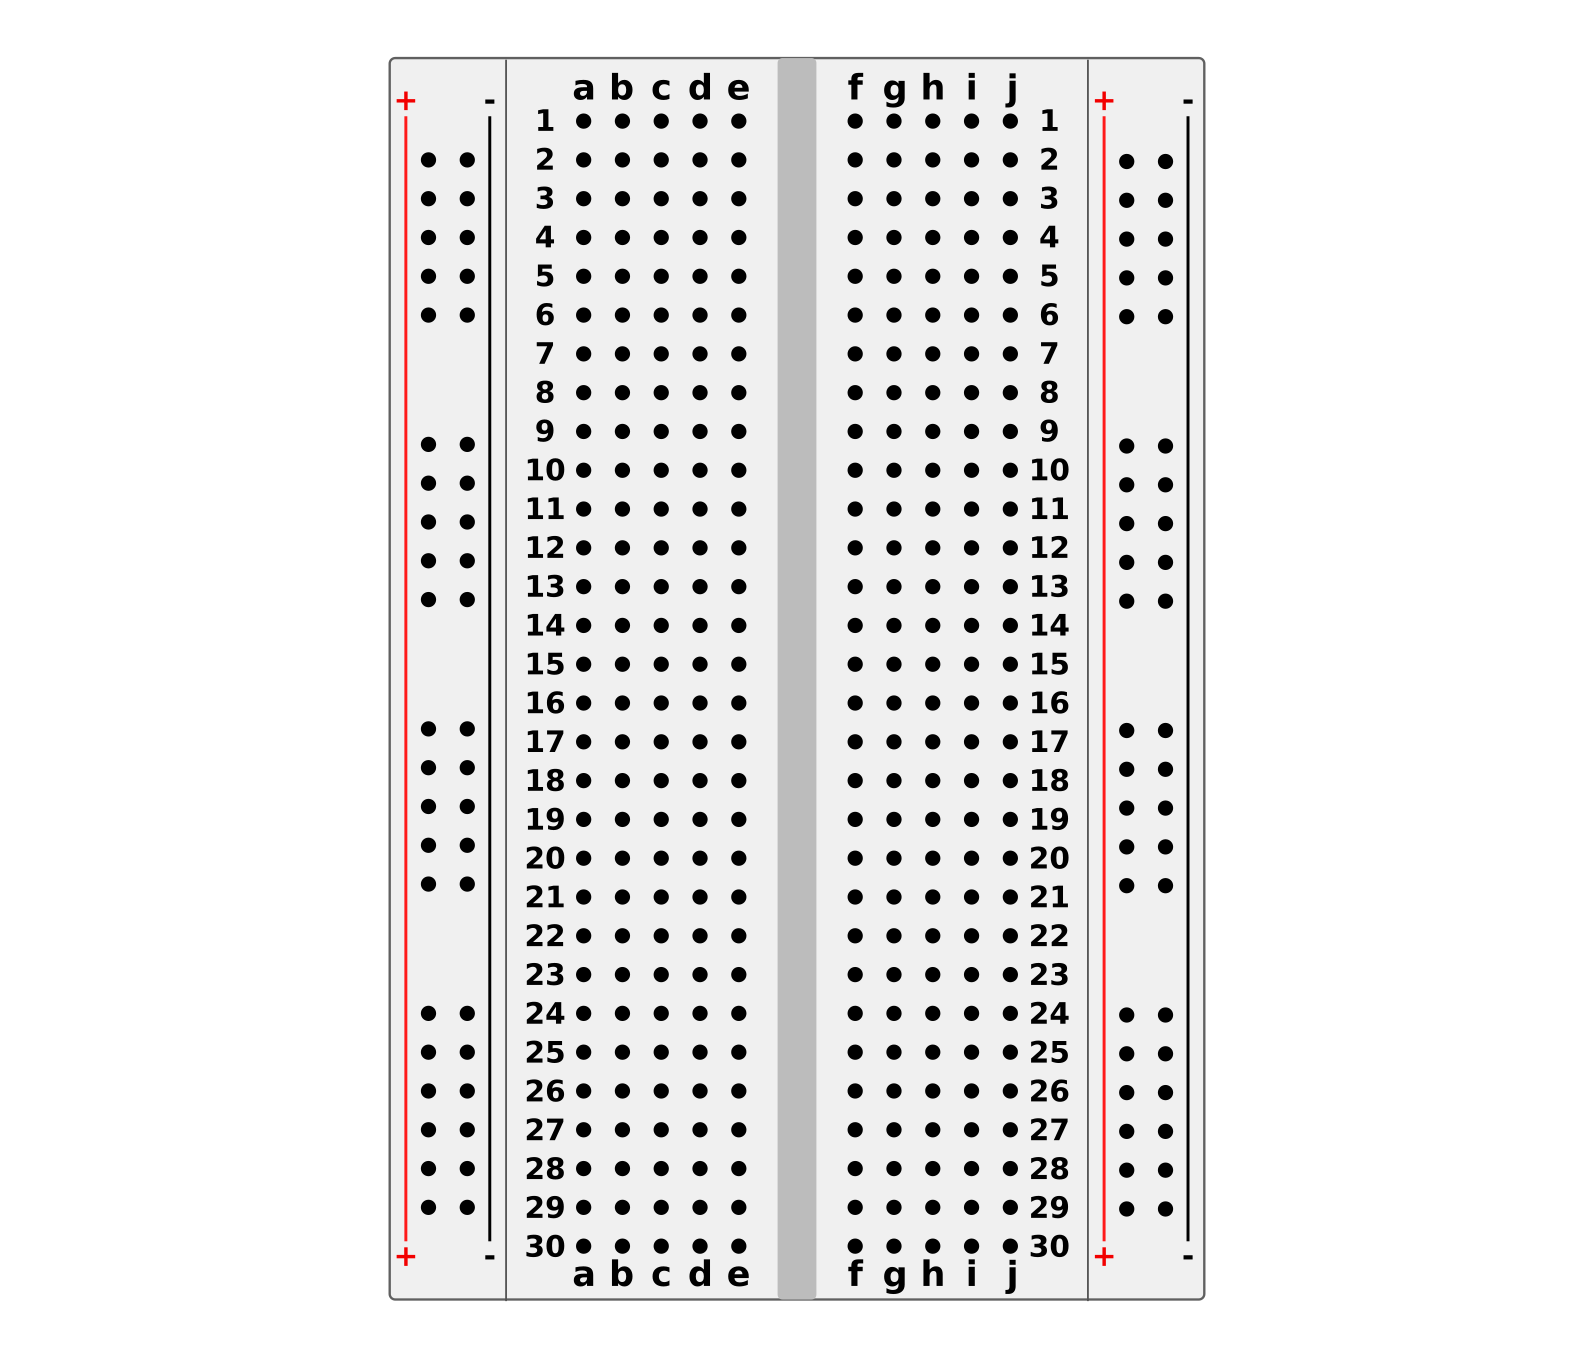
\includegraphics[width=0.5\textwidth]{breadboard}

Internally, it is just rows of interlinked metal, which connect/ bridge pins together. As seen, there are two sets of 30 rows of 5 pins, with each pin on rows connecting. Two connecting parts should be on the same row. There are also power rails, which allow for 2 different \gls{vltg}s, and two sets of ground pins. These are convenient to access, but not the only suitable pins for providing power. Breadboards are specifically meant for DIP components, with the gap in the centre allowing for DIP chips to be placed, separating each of their pins. Components can be connected with male to male jumper wires. As mentioned, it is worth only attaching power when you are sure that everything is firmly connected, with no potential for shorts. There are limits to the suitability of a breadboard circuit, which are meant for lower power and lower speed circuitry.

\Examples{Examples}

Here are a range of example circuits to help you understand how a breadboard circuit should be wired, with increasing complexity.

The first example is an LED with a resistor, a button, and a battery.

\Quiz{Challenges}

1. Connect a circuit with a blue 5mm led, 2 AA batteries, a 50$\ohm$ resistor and a momentary push button.

2. Connect a circuit with 2 AA batteries, with a blue LED, resistor and button, in parallel with a red LED, resistor and button. You will need to calculate the resistor required.

Here are a range of challenges, to build up your confidence. You may need to read other sections of this course if you are struggling.

The next stage from here is a proto-board design, using vero or strip board, design of a custom circuit board, or using existing modules suitable for the design. The cost of custom printed circuit boards has decreased considerably in the past few years, through sites such as JLCPCB. This has made custom PCB design a more viable option for field use.
In the further reading section, there is detail on PCB design and related resources, but it is not a key course focus.

\subsection{Soldering}

Being able to solder is an important skill to have. Usually, someone would first make a circuit using DIP components before attempting more challenging SMD components.

Soldering is the process of creating a metal joint between a component and a circuit board, to allow for a considerably improved electrical, mechanical and thermal connection. Solder is typically in wire form, but can also be in paste form, and it is a metal with a low melting point, allowing for a quick connection to be made with a reduced risk of damaging components.

\includegraphics[width=0.5\textwidth]{solderingiron}

The most basic form of soldering uses a soldering iron and solder wire. It is recommended to use a holder, to hold the parts in place, to free up hands for soldering. The soldering iron should be placed, so it heats the metal of the component and the interface metal, with solder wire placed at the other side so the solder can bridge them, making a clean connection. A clean connection should have a clean flow between the parts, rather than a ball of solder or poor joint.

\includegraphics[width=0.5\textwidth]{soldering}

\includegraphics[width=0.5\textwidth]{solderjoints}

Sometimes too much solder may be added, which can be difficult to remove. A solder sucker can help, where you remelt the area with excess solder and quickly press the solder sucker just above, which uses suction to remove excess solder. Solder wick is another option, which I prefer, as you place it between the excess solder and your soldering iron, where it "wicks" up the additional solder. This tends to be copper, with high heat transfer, so keep hands further from the iron.

Soldering temperature is important. It is worth looking at the melting point of the solder you are using, with lead-free solder typically having a slightly higher melting temperature of around 217C, depending on composition.

Although lead-free solder is known to be slightly more difficult to use, being better for the environment and for your health for me makes it the better option. I haven't found too high a difficulty jump, especially if good quality equipment is used. Also it would be more beneficial learning what's used in commercial/public products, and shouldn't be phased out.

\section{Electronics safety}

Safety is a key consideration when doing anything with electronics. If you are unsure, it is always best to ask rather than to assume.

As discussed, current is related to \gls{vltg} and resistance through $V=IR$. The body has a resistance which can vary depending on length etc, but is relatively high (this can decrease significantly from water/ high Humidity). Therefore, as \gls{vltg} increases, so will current if the resistance stays the same. You should always take sufficient precautions when using electronics, but especially when dealing with higher \gls{vltg}s, where it can be fatal. The in-person practical elements use low \gls{vltg}s, which are much safer. It is important to know when you don't have the knowledge or resources for a given piece of electronics and when it may be the better option to have someone else repair it. You should also consider that sometimes the best option is to replace something rather than repair it, such as when it may be dangerous, could end up costing you more if it isn't reliable, or takes a considerable amount of time to fix.

Component ratings are often not initially considered but are very important. Knowledge of ratings ensure that a selected part can take the expected power loss without damage. Therefore, it is important when selecting a resistor to calculate its estimated power drop, and select a resistor with a power rating clearly above the max predicted power losses. It is important to add a safety buffer, as circuits in reality are not ideal, so may react slightly differently than expected, such as a component having a resistance value that differs from its value.
Tolerance is the percentage at which a value can differ. This is usually under 20\% (it can be considerably smaller). If you are unsure, it is better though to add a safety buffer, double the calculated value is fairly common, as it helps to account for how the tolerances of other components affect that one.

It is important to consider that all components have losses, including wire, so this needs to be considered, with a wire or connector of suitable ratings selected. With this waste heat, also comes a \gls{vltg} drop, which may also be a factor, as if high enough, can cause issues with the circuit itself.

For wires, you have different wire gauges, and sometimes different materials. Typically wires are copper, but sometimes are aluminium, with a resistance around 64\% higher than copper, so looking at wire gauge alone isn't enough. In general, there are standardised values for what current flow is suitable through a given gauge of wire. Again, it is helpful to keep the chosen wire a fair bit above the power rating you require, considering that only just meeting those ratings will lead to considerable losses in the wire. And if there are cost constraints, it is important to consider that a thinner wire, which is initially cheaper, may end up costing more due to electrical losses.

There are a range of connectors, and depending on the application, will have their own ratings. Mechanically connected, such as screw terminals, are likely to have a resistance higher than directly soldered, but can give more flexibility to make alterations.

You should be careful when handling components, as built up static can cause damage. Grounding yourself, such as touching a metal surface, can help to reduce this static potential. Anti-static wrist straps are something that can be sourced cheaply to limit the potential of causing damage.

Soldering may be something that is required for a project. Health risks are associated with all forms of soldering, so you should always solder in a well-ventilated area with suitable equipment. If possible, although slightly harder to work with, it would be recommended to use lead-free solder, reducing health risks and allowing for safer use in the field. Flux is used in solder, to help it flow, but its evaporation produces a vapour which can be harmful if inhaled. Many soldering iron setups have extraction next to the iron, to minimise this chance of inhaling it.

Before connecting wires, particularly at higher \gls{vltg} levels, running your hand along a cable to check for potential damage is important, replacing a cable if this is the case. It is also good practice to ensure both sides of equipment being connected are turned off before and during wiring, to prevent potential sparks, damage or electric shock.

Certain components can still be dangerous regardless of whether they are powered. Capacitors are an example, which still hold power after a circuit has been turned off, for a period of time. Therefore, ensure not to touch or short one in a circuit. It is good practice to have bleeder/ discharge resistors connected at either end of high \gls{vltg} capacitors so that when not powered, over time they will discharge. This will add some inefficiencies to a system, but improves safety.

As previously mentioned, it is important to ensure components aren't shorted, which can cause damage quickly as the source will pump as much current as it can into the part, causing fast heat up. Storage of components, such as batteries in a proper case, is important to ensure that they cannot get shorted. Checking soldered circuits to ensure nothing is bridged, such as using a combination of a microscope/ magnifier, and using a multimeters continuity checker, as mentioned previously, is a worthwhile exercise.

\section{Important considerations}

\subsection{Component footprints}

Components can be found in many footprints, which needs consideration in design or repair. Imperial measurement is commonly used for surface mount resistors, capacitors and inductors, with values in mils, representing a 1000th of an inch. In many cases surface mount components are used in commercial products, so may be required in product repair. Understanding their size, and your ability to solder them is important. You may be able to access a soldering oven, which can help make this process easier, considering that as solder melts, it can somewhat help to pull a component into place, if it is marginally off-centred.

Components are only rated for a certain amount of heat, so care should be taken to limit thermal damage. If a component with multiple pads is being done, leaving time between soldering pins helps to prevent heat build up.

\subsection{Supply Chain issues}

Since the Pandemic, there has been many supply shortages and stock issues. This has been worsened by some companies/ institutions beginning to purchase components in excess to ensure they had what they needed. Being aware of this is key in electronics design, especially when a certain project may need replicating in the future.

You should consider stock at the beginning of a design project, and ordering parts early if you know they are needed, rather than waiting for design completion, as by that point it could be out of stock. The main issue is with specialised ICs and Microcontrollers, less so with passives/ discrete components, which can likely be ordered once you know specific requirements. A similar mindset should be followed for modules though, as they often have parts with low stock.

The parts shortages started in 2020 are some of the worst that have been seen, mainly affecting silicon components. There was a combination of factors which kick-started it. These included increase in demand for electronics, pandemic related shipping delays, natural disasters/ fires, vast increases in the price of silicon and trade disputes. The market naturally goes through periods of higher and lower supplies, with early 2020 meaning to be a period of lower supply, further worsening things. The situation has slowly been improving.

Tips could include to use discrete or widely available parts over specific or niche ones where necessary, or modules where there are similar alternatives available.

Digi-Key has a small lead time trends page. It is useful to be aware of lead times for a given part, and how they might vary. \href{https://www.digikey.co.uk/en/resources/reports/lead-time-trends}{Link}

TTI also has a similar tool, with viewable graphs too. \href{https://www.tti.com/content/ttiinc/en/apps/lead-time-trends.html}{Link}

\subsection{Environmental considerations-}
There are two sides to environmental considerations. First, ensuring a product is suitable to the environment it is placed in, and second ensuring the design of the project has a limited carbon footprint or use of scarce, conflict, or toxic materials.

You should aim to use all RoHS certified components, luckily being most modern components. RoHS restricts the use of harmful materials such as lead within electronics. Solder is not always RoHS certified, as lead-based solder is still commonly used, especially with prototypes. Lead-based solder tends to be a mix of tin and lead, whereas lead-free substitutes the lead for some of the following: copper, silver, nickel and zinc, among others.

One way to somewhat reduce the carbon footprint could be choosing a smaller footprint, although for silicon products, this would only make a minor difference since it is likely that the silicon wafer fabrication is a large proportion of the overall carbon footprint.

There are limited steps in reducing carbon footprint within sourcing. Buying local will have an impact, but it's likely that they sourced the parts from long distances, anyway. Therefore, it is worth focusing on the longevity and reusability of parts. If designing a circuit board, using pin headers for modules to slot into means that the modules can be reused, or replaced if there are faults, rather than the whole unit.

There is a range of aspects regarding placement, such as whether waterproofing or cooling is needed. You should consider that rated temperature values are usually in ambient temperatures of around 25\degree C, so an enclosed part with poor thermal path, close to its rating, could fail over time. You may consider whether active or passive cooling is needed, such as a copper or aluminium heatsink, along with a fan if actively cooled. If a fan is used, the circuit enclosure should have air intake and outtake. Some component footprints may have heatsinks specifically built for them. Thermal design/ thermal relief can be factored into PCB design too if needs be.

There are online calculators for figuring aspects such as thermal design, that are more time effective than learning thermo and fluid dynamics.

\subsection{CAD and Material Design}

You often require an enclosure for use of electronics in the field. Therefore, understanding different types of processes for their design would be useful.

Some of the main techniques for prototyping include 3D printing, laser cutting, and CNC milling, techniques widely used for quick prototyping of an enclosure.

3D printing mainly uses plastics, depending on the application. The most common is PLA (Polylactic Acid), a plastic derived from plants such as Corn. It is biodegradable and compared to most other plastics, has lower contamination risk. A problem is its low glass transition temperature (~60\degree C), which means at lower temperatures it warps, so may not be suitable in direct sunlight for sustained periods.

Lasercutting is suitable for some types of enclosure design. Depending on laser type and power, a range of different materials, from plastics like acrylic to wood can be cut. It is a good approach when quick and less complex parts are needed.

CAD Milling is a subtractive process where material is removed rather than added. Therefore, it is a wasteful process but allows a strong piece to be produced in a wide range of materials, including metals. Depending on the machine, there are limits to possible geometries.

There is a range of project enclosures meant for electronics projects, which can be sourced relatively cheaply, so are also worth considering to save time. These are typically seen in materials such as metals like steel or plastics like ABS. Some of these are IP rated, so can withstand different levels of water.

\subsection{How to find a part}

This is an important skill, especially in a changing market with parts sourcing causing many problems. You should first understand what you need, to then figure whats available. It is useful to remember that a part with your specific requirements may not be available, so consider bounds a part could work between, or whether circuit alterations are required to find parts. Remember, multiple parts can be used in series or parallel to get the equivalent value, ensuring other factors are considered.

I will quickly talk through the processes needed for part selection. This is done in detail for a particular part, and in less detail with other parts, as different components have different characteristics which are important. For this I will use DigiKey, as it a major components supplier, although it may not always be the cheapest, it is known to have one of the better "search engines". Therefore, once you have found the parts you could use, you can then check other suppliers or comparison tools such as Octopart.

I will give an example part, being a resistor. Let's say I am designing a basic LED circuit, where when a button is pressed, the light turns on. It needs to use a 3.6V LIR2032 (a small rechargeable coin cell), and it needs to be a red LED. I have been told it should have a current consumption of 25mA, with a  1610 footprint. I have been told it needs to be in the colour white. I have been told it should be 1206 size (considering that this represents a size of around 0.12*0.06 inches or 3*1.4mm).
Therefore, the first step you can do is open up the DigiKey homepage- \href{https://www.DigiKey.co.uk/}{Link}

\includegraphics[width=0.5\textwidth]{screenshots/DigiKeyHome}

There are many categories with subcategories within the products section, on the left-hand side. This is useful when we know what category is needed, but takes some time to learn, particularly when different sites categorise things differently. Therefore, you can instead use the search bar at the top centre, type LED, and press the search button.

\includegraphics[width=0.5\textwidth]{screenshots/DigiKeyHomeLEDSearch}

It usually shows top results, each with a link and image, as well as listing the number of suitable parts. As seen, there is a white LED subsection, which is ideal.

\includegraphics[width=0.5\textwidth]{screenshots/DigiKeyLEDSearched}
\includegraphics[width=0.5\textwidth]{screenshots/DigiKeyWhiteLEDSectionFound}

This opens a page with a lot of information, so it may initially be overwhelming. At the top, there are scrollable filters to see whats available specifically for our requirements. Below, there are checkboxes for specific but often important search criteria, with the parts shown below this.

\includegraphics[width=0.5\textwidth]{screenshots/DigiKeyWhiteLEDPage}

On the top right of the criteria, I would recommend setting the filters to stacked, to see all filters at once, to go through each methodically.

\includegraphics[width=0.5\textwidth]{screenshots/DigiKeyWhiteLEDPageStacked}

Many of these you will not need or may not understand, which is okay. You just need to scope out the specific characteristics which are important. Since some chips may have multiple LEDs on one die, firstly, it would be beneficial to find "\gls{vltg}- Forward", and select between the lowest number until 3.6V as a maximum, you can hold click to select a range, or click on the lowest boundary, and then scroll to find the highest suitable boundary and shift-click on it.

\includegraphics[width=0.5\textwidth]{screenshots/DigiKeyWhiteLEDPageVoltage}

Then the next suitable section looks to be maximum current, since we will likely use a resistor to limit current anyway, the maximum could be higher than 25mA, since running a component at its max rated power can decrease its longevity. Therefore, we could select between the minimum value and 40mA.

\includegraphics[width=0.5\textwidth]{screenshots/DigiKeyWhiteLEDPageCurrent}

We can then use "Package/Case", to look for the 1206 package size. You can then pick Apply Now. With the components shortages, it may be useful to select "In Stock", and also select RoHS compliant for environmental reasons.

\includegraphics[width=0.5\textwidth]{screenshots/DigiKeyWhiteLEDPagePackage}

We can now see the available options. You should see available stock, and cost in different quantities, along with other data, such as the CCT value for the colour, depending on the shade of white needed.

\includegraphics[width=0.5\textwidth]{screenshots/DigiKeyWhiteLEDPageOptions}

Although the stock number may seem a lot, for industrial customers producing many products, this might be a tiny amount, so selecting a part with plenty in stock if you feel you may need more in the future is important. I have now selected the final part.

\includegraphics[width=0.5\textwidth]{screenshots/DigiKeyWhiteLEDFinalPart}

To know what resistor we may need to select, we should check the datasheet. For an LED, you can find the forward \gls{vltg} vs forward current graph. We can see at 25mA, the forward \gls{vltg} is around 3.25V. Therefore, we need to drop a \gls{vltg} of 0.35V in a resistor. The ratio between the forward \gls{vltg} and resistor \gls{vltg} is 9.285714286. Given that the resistance of the LED will be $R=V/I=3.25/0.025=130Ohms$. With this ratio, we need a resistor of around 14$\ohm$s. Sometimes an exact resistance value isn't available, so an alternate value may be required. You should ensure that it is as close as possible and if there isn't something close enough, you can use the parallel resistor formula/ use multiple resistors in series.

As we have talked about needing a resistor above, we can try to find one. Rather than having predetermined specifics, we can use the data derived from the LED requirements. There will be around 25mA through the resistor, meaning power of around 0.00875W. As previously mentioned, it can be worth doubling this value to be clear of its max ratings, so we are looking for a resistor of at least 0.0175W ratings. Here, I am going to say that we don't mind what size it is, but want a cheap option. We want a resistance as close 14$\ohm$ as possible, in this case a tolerance of a maximum of 1\% (Often 5\% is used, for non precision applications). We have been told it must be a surface mount part. Luckily, in this case, Resistance, Tolerance and Power are next to each other.

\includegraphics[width=0.5\textwidth]{screenshots/DigiKeyResistor}

We want to ensure its available and that it is at least 0603 for hand soldering. A part is selected with plenty in stock, with all the ratings we would like, while being a cheaper part.

\includegraphics[width=0.5\textwidth]{screenshots/DigiKeyResistorSelected}

You should remember that sites such as DigiKey are not always the cheapest, with this resistor costing £0.08. Although this sounds cheap, when hundreds of parts are required, this quickly adds up. Sites such as LCSC have parts such as resistors for considerably cheaper, but has a worse search engine and filters, along with typically slower delivery times. You need to factor shipping costs into the overall costs, as well as import charges.

Now, a button suitable for the task should be found. It needs to take a current of at least 25mA, and a \gls{vltg} of at least 3V. In this case, we are budget-constrained to under £0.20, so a tactile switch would be the best option. A switch has been found, rated for 50mA, (again using a times two safety buffer), to account for plenty of unexpected deviance.

\includegraphics[width=0.5\textwidth]{screenshots/DigiKeyButton}

We have now selected several parts, using just the criteria required. There are many other filters that can be selected. As already mentioned, DigiKey has plenty of components on offer, and a good search function, but is certainly not the cheapest option. It can be used to get a better idea of what you are searching for, to then search elsewhere, such as Octopart using a specific part number.

This section quickly discusses some of the key factors and variables you should consider for a range of parts.

You should consider that power and current ratings sometimes regards the peak power seen but sometimes the average. \gls{vltg} ratings usually relate to peak \gls{vltg}s.

Resistors- Resistors are basic components, but still have many filters, with key ones touched upon now. Resistance is obviously key. Tolerance is the max percentage deviance with the resistance, so lower is better. Power is its max power rating usually at ambient temperatures. The temperature coefficient is how much its resistance can change due to a temperature change. Package or footprint is regarding its size and the specific footprint as mentioned in the datasheet.

Capacitors- Capacitors have a few similar characteristics such as tolerance etc. Factors include ESR similar to impedance, which is the internal resistance at a given frequency, \gls{vltg} rating which is the max \gls{vltg} it can be charged to, ripple current is the current it can withstand at a given frequency and polarity, as some capacitors are restricted to a single direction for current flow.

Inductors- These have a few of the same criteria already mentioned, a key criteria being its current rating, which is the maximum current the inductor wire can take (constantly/ on average) and saturation current, which is where the magnetic field is no longer proportional to current.

\subsection{Reading Datasheets}

Sometimes going off filters or parameters of parts search engines isn't enough, particularly for integrated circuits where extra passive or active components are required for their operation. Therefore, this section quickly goes through looking through datasheets, with some specific part examples.

Like the section above, you should remember that there will be a lot of information in datasheets, a lot of which you might not understand, with the likelihood being you don't need to understand the vast majority of it. There is a skill though to be able to pick through all this, to find out what you do need to know.

\subsection{Finding Arduino Libraries}

Arduino IDE is a widely used development platform, particularly for DIY projects. This makes it considerably easier to find libraries for a specific chip or module.

Often, going onto the page for a module should give details on its usage, as well as how to install libraries.

The Arduino IDE has a built in libraries search tool, which should have many of the more common ICs/ modules.

\subsection{Circuit Design Process}

Now that you have seen many components, this section discusses some techniques, tips, and processes involved in circuit design.

It is important to first consider what your requirements are. What function does the circuit need to have, what environment should it be suitable for, what budget should it adhere to, what interaction does a user need to have with it, how easy will it be to make, can parts actually be sourced for it, and what restrictions are there regarding input power, how much processing power is required, how easy should it be to program, are there any niche libraries needed for it. These factors will be split and discussed individually in some detail. Remember that it is hard to get a "perfect" circuit. There are many variables and factors at play. It is a balancing act of figuring out which factors are most important for the project.

As a first tip, I would recommend writing answers to the above questions, and then writing "nice to haves" for that factor, and what is needed for a "minimal viable product".

First, figuring out what function is required, will dictate what type of components are needed. It is worth seeing if there are existing circuits which do what you need or similar. An example could be checking for open-source designs which could be adapted for your specific use case.

Regarding what environment it needs to be suitable for, there are multiple factors. These include areas such as does the enclosure need to be waterproof? Does there need to be a heatsink or fan due to high expected temperatures? Does it need all SMD components to be low profile? Does a specialist circuit board need producing to adhere to certain standards? What fail-safes need to be integrated into the design?

Considering the budget, it is worth leaving a large safety buffer, as there needs to be extra in case there are issues in the first design. You need to factor in that multiple parts may need purchasing if there is a minimum order quantity. You should also consider whether the budget would be restrictive for what needs to be done. It is important to figure out whether saving money or saving time is more important, such as whether using modules or custom designs would be better. There should be some wiggle room in the budget, to account for unseen factors.

You need to figure out what interface it needs for someone to use it. This could include considering whether it needs to transmit data through a wired or wireless protocol? Does it store data on an SD card or inbuilt storage that needs connecting to a computer? Does it have a small display and buttons for setting it up, or is a computer or external device required?

Depending on its complexity, you need to consider whether an external service should solder the board, whether you do it by hand or whether a heat station should be used. This may make you focus on a specific design, such as using DIP components or focusing on SMD components.

A more important question than usual is, can components actually be sourced? There are tips elsewhere in this course on the matter, being a key parameter. Sometimes more novel approaches may need to be taken, if the typical route is not viable with parts shortages. Having a quick feel on stock levels for necessary parts is a worthwhile exercise before getting too far into a design.

It is important to be aware of how power needs may restrict the design, whether it is for mobile uses, with a restriction on how much power components can use, while ensuring that high-efficiency parts are selected, or whether there is only a specific \gls{vltg} input, so deciding what power conversion circuitry is required and viable.

Selecting what microcontroller to use is important. Certain platforms, such as those compatible with the Arduino IDE can help to speed up design. This is due to a wide availability of libraries and easier-to-use code. Within different platforms, there are microcontrollers of varying performance, so understanding your needs regarding this is important. This could relate to whether an 8 bit, 16 bit or 32 bit microcontroller is required, the latter of which should work for most end cases.

\section{Further reading}

This section provides reading into advanced topics. Although you may not make a circuit with the below, understanding them may be beneficial. The below ideas may help you to solidify your understanding of the key theory mentioned above.

\subsection{Rectification}

\Theory{What is Rectification?}

Rectification is the process of converting AC to DC, commonly used in power supplies, such as a phone or laptop charger. This is because digital electronics require DC to function. Although diagnosis of AC circuits should not be done without the necessary training, understanding of how AC circuits function is important for safety and to better understand the use of components.

\textit{This circuit uses components which have already been discussed earlier in this document, so for further explanation, refer back to the appropriate sections.}

For this AC-DC conversion, the alternating current needs to be converted to flow in just one direction. Therefore, a key component in this process is a diode.

The most basic form of rectifier is a half-bridge (otherwise known as half-wave). This uses a single diode in series with the load, to limit current flow to one direction. Therefore, the output wave is the positive side of the sinusoidal wave, with the average output \gls{vltg} around half of the RMS \gls{vltg}, although in a form unsuitable for most DC circuits.

\vspace*{1\baselineskip}

\includegraphics[width=0.5\textwidth]{halfbridge}
\includegraphics[width=0.5\textwidth]{halfbridgewave}

\vspace*{1\baselineskip}

A half-bridge circuit can be improved through use of filtering, with the addition of a capacitor to smooth the output \gls{vltg}. This capacitor is added in parallel, where it is charged by the input, which it then outputs when the \gls{vltg} drops below its own \gls{vltg}. This enables an output \gls{vltg} closer to a smooth DC \gls{vltg}. As previously mentioned, even if perfectly smoothed, the max \gls{vltg} that could be attained is half the RMS \gls{vltg}.

\vspace*{1\baselineskip}

\includegraphics[width=0.5\textwidth]{halfbridgesmoothed}
\includegraphics[width=0.5\textwidth]{halfbridgewavesmoothed}

\vspace*{1\baselineskip}

A full-bridge rectifier is a further improvement. These use four diodes, meaning that whichever way the current flows at the input, it will be fixed at the output. Therefore, there will be a sinusoidal \gls{vltg} magnitude, but only in the positive axis. This can again be smoothed with a capacitor, and if efficiently smoothed, will have an output close to RMS.

\vspace*{1\baselineskip}

\includegraphics[width=0.5\textwidth]{fullbridge}
\includegraphics[width=0.5\textwidth]{fullbridgewave}

\vspace*{1\baselineskip}

\includegraphics[width=0.5\textwidth]{fullbridgesmoothed}
\includegraphics[width=0.5\textwidth]{fullbridgewavesmoothed}


\Examples{Example circuits, applications and considerations}

This section will quickly look at applications of the above mentioned circuits.

Rectification circuits are widely used, especially for AC-DC power supplies, as an initial stage to convert AC to DC. Therefore, their main use is within mains connected power supplies. Another example is a dynamo torch, where the AC power from the generator needs rectified to power an LED.

It is likely that in most cases a full-bridge rectifier would be used rather than a half-bridge rectifier, unless initial costs were a major consideration.

Because of variance in the manufacturing process, even within a single product, it is commonly considered best practice to use a full-bridge diode package, where there are four equal diodes within one part.

Rectifiers are generally used as part of a more complex power system, usually as an earlier stage.

\Simulation{Simulations}

Below are several simulations to have an experiment with to help your understanding of Rectification.

Half-Bridge rectifier at 230V RMS, 50Hz- \href{https://tinyurl.com/24lw5qjj}{Link}

Half-Bridge rectifier at 230V RMS, 50hz with capacitive smoothing- \href{https://tinyurl.com/27lb3k8o}{Link}

Full-bridge rectifier at 230V RMS, 50Hz without smoothing- \href{https://tinyurl.com/224uqhfw}{Link}

Full-bridge rectifier at 230V RMS, 50Hz with capacitive smoothing- \href{https://tinyurl.com/2yeg4kof}{Link}

\Quiz{Quiz}

1. What is the main benefit of a full-bridge rectifier over a half-bridge rectifier.

a) It is cheaper to build.

b) It allows for full utilisation of the input \gls{vltg}.

c) It uses fewer components.

2. Why are smoothing capacitors useful? (There may be more than one right answer)

a) They allow for a more constant output \gls{vltg}.

b) They increase average power output.

c) They reduce output ripple.

3. True or False, it is known to be better to use several diodes individually rather than packaged together as a full bridge rectifier package.

4. True or False, rectifiers can be used to also convert DC to AC.


Challenge- Using Falstad or hand drawn, design a full-bridge rectifier with \gls{vltg} variance/ ripple lower than 10\%, working with an AC \gls{vltg} of a peak value of 326V, at 50Hz.

\pagebreak

\subsection{Gate Driving}

\Theory{What is Gate Driving?}

Gate driving is necessary for using MOSFETs in high-speed circuits. As mentioned earlier, MOSFET gates have an inherent capacitance which requires charging in order for the gate to “open”. Therefore, for fast switching, it may require large amounts of current, which a microcontroller usually can't supply. Therefore, there are integrated circuits with common methods to allow for these to be charged safely. A common simpler methods is called a totem pole gate driver. This uses two BJT transistors, one used to charge and the other to discharge the gate. BJTs are used because of their simplicity and ability to amplify the input current using an external source. Even then, it is important to use a resistor to limit the gates charge current.

This section references a range of components and knowledge from the main sections of the course, to help consolidate past theory.

Here is a circuit of it in action, feel free to play around with it- \href{https://tinyurl.com/2m77d6zl}{Link}

\includegraphics[width=0.5\textwidth]{gatedriver1}

The method shown above isn't the only viable option, but is one which is widely used and one of the simpler methods to understand.

\subsection{555 Timers}

555 timers are adaptable ICs, for a range of timing techniques, that may not require a whole microcontroller. Although understanding the internal structure of a 555 timer is outside the course scope, understanding how and why they are used could be beneficial.
Depending on how it is connected to, it can output waveforms of different frequencies, or as a timer.

\subsection{Motors and Generators}

Motors and Generators use a set of physics principles in their operation. Motors convert electrical energy to kinetic (typically rotational), where generators do the reverse.

They operate due to the motor effect which is the following. A current carrying conductor will induce a magnetic force, which will interact with other magnetic forces. If the conductor is free to move, it will. Therefore motors are designed using both electromagnets and permenant magnets with interacting magnetic fields to cause rotational movement.

The reverse is also true, when a conductor moves through a magnetic field, a current is induced. A large proportion of electricity is generated using a generator, where usually steam from either a combustion process of oil, gas or coal, or from nuclear fission, causes the evaporation of steam, the movement of which causes a generator to turn, thus generating electricity.

\subsection{Renewable Electricity}

Renewable Electricity is of increasing importance, as we look to reduce our carbon footprint. This section quickly looks into different methods, and how they work.

It is important to consider that all renewable energy sources have a carbon footprint, and this can vary significantly from manufacturer to manufacturer. As shown \href{http://www.solarscorecard.com/2018-19/2018-19-SVTC-Solar-Scorecard.pdf}{here}, how sustainable a manufacturer is can vary considerably, so it would be better to select panels from a manufacturer at the top of a list such as this.

Solar panels are diodes, working like a generator (with the photovoltaic effect), where solar radiation induces a current and therefore electrical energy. These are produced using semiconducting material, such as doped silicon.

\includegraphics[width=0.5\textwidth]{solarpanel}

Most other renewable methods involve a motor acting as a generator. Whether it is wind power through wind turbines, where blades are connected to a motor to generate wind power, or hydroelectric, where flow of current against the sea or through a dam spins rotors. Hydroelectric, especially using dams has a mixed record, because of its fairly significant impact upon the environment and nature. Geothermal uses heat from within the ground to heat up steam, to push rotors of a generator.

\subsection{PCB Design Basics}

Although this isn't in depth PCB design, it is a few useful to know tips.

The cost of custom PCB production has reduced considerably due to the increase in prototype PCB services. JLCPCB was one of the first low cost options. The reason their model is viable is that they use excess board space, left from larger customers, so most costs are due to the set-up, rather than the material costs. It also means that it is reducing waste, and possibly carbon footprint.

A couple of free PCB design tools include EasyEDA and KiCAD. If you prefer open-source software, KiCAD is a good option, otherwise, EasyEDA is pretty easy to get started on, is free for even its advanced features, and has links to LCSC and JLCPCB to get you going quicker. Lots of time can be spent finding suitable package footprints or designing footprints. EasyEDA simplifies things, with most parts in LCSC's library being available to search for and drop into the design. Even if it is an external part, there are many community part footprints and schematic designs. For community derived parts, it is worth reading the datasheet to ensure it matches up with that design. Most datasheets should provide information on suitable PCB footprint design.

\section{Resources}

There are many electronics resources for further learning. Particuarly useful resources are referenced below, with their purpose.

\subsection{Manufacturers}

It is handy to know reputable manufacturers of components and modules. This is not definitive, but provides a trustworthy list. This focuses on larger manufacturers, but there are many more trusted manufacturers. Keep in mind that there are fake components in the market, so ensure you source parts from a trusted supplier, talked about in the section below! As touched upon in the finding components section, most parts through a site such as DigiKey should be reliable.

Resistors- Yageo, BOURNS, Panasonic, ROHM, Samsung, TE Connectivity, Vishay, Walsin.

Capacitors- Rubycon, Panasonic, Hitachi, Sanyo, Vishay, Nichicon, NCC, Wurth, Illinois Capacitor, Cornell Dubilier.

Inductors- Wurth, Walsin, Vishay, TDK, TE Connectivity, Pulse Elec, Murata Electronics, BOURNS, EATON.

Transistors- Vishay, TOSHIBA, Texas Instruments, STMicroelectronics, ROHM, RENESAS, onsemi, NXP Semicon, Nexperia, Infineon, Diodes Incorporated.

Diodes- Vishay, TOSHIBA, STMicroelectronics, ROHM, onsemi, Nexperia, Microchip Tech, Infineon, Diodes Incorporated.

\gls{snsr}s- Infineon, Analog Devices, OMRON, Texas Instruments, TE Connectivity, NXP, Microchip Technology, Murata, BOSCH, STMicroelectronics.

Microcontrollers- Microchip, ATMEL/AVR, NXP, STMicroelectronics, Espressif Systems, Infineon, Altera, Raspberry Pi, RENESAS.

ICs- Texas Instruments

\subsection{Suppliers}

Starting with several trusted parts suppliers.

Arrow Electronics- Europe based electronics components shop.

RS Components- UK based electrical and industrial components shop.

Mouser- US based electronics components shop.

Farnell/CPC- Electronics components shop based in several regions.

LCSC- Electronics components shop based in China, with links to JLCPCB and EasyEDA, offering lower costs than most other suppliers for larger orders.

Digi-Key

Rapid- UK based electrical and industrial components shop.

EuroCircuits- Lower cost PCB manufacturer based in Europe.

JLCPCB- Low cost PCB manufacturer based in China

Aisler- Lower cost PCB manufacturer based in Europe.


Most the above focus on singular components, which may not be what you are looking for. If you are looking more for modules or DIY components, here are a few trusted retailers.

HobbyTronics- UK Based hobbyist electronics shop.

Bitsbox- UK Based hobbyist electronics shop.

Adafruit- US Based company producing a range of boards/ modules.

Sparkfun- US Based company producing a range of boards/ modules.

Pimoroni- UK Based module maker and hobbyist electronics shop.


There are a couple of sites used to find stock of components across suppliers, while comparing their costs. Within these tools, there are multiple suppliers mentioned, a few of which being resellers, where you may pay more, but they often have parts in tight supply.

These could be thought of Electronic Part Search Engines.

Octopart

Findchips

OEMSecrets

EasyBom


\subsection{Electronics Software}

There are several bits of electronics software mentioned below, whether it is for simulation or PCB design.

Falstad- Free online electronics simulation program, which is easy to visualise what is happening in a circuit.

LTSpice- Free and powerful electronics simulator, although slightly dated presentation, produced by LT.

TinkerCAD- Simple online software for basic 3D design and electronics design/ simulation.

MicroCap 12- Although it can be seen as abandonware, it is now free, relatively recent and a powerful piece of software.

KiCAD- Free and open-source PCB design package

EasyEDA- Free and easy-to-use PCB Design Package with links to both LCSC and JLCPCB.

subsection{Further learning sites}

Another helpful resource could be additional places to go to learn further.

Allaboutelectronics

Hackaday

Hackster.io

There are a range of helpful YouTube channels, such as the below:

GreatScott- Page with many tutorials and projects, in plenty of detail, although it can be complex for beginners. If you like learning through a project-based ideas, it's worth checking out.

Electronoobs- Another project based channel, teaching you a range of things.

EEVBlog- One of the biggest electronics video blogs, covering a range of areas, from an Electronics Engineer. Known to be unscripted, and "off-the-cuff", but informative.

Adafruit Industries- Channel set up by Adafruit, discussing electronics and their modules.

\section{Necessary software}

In this document, you are encouraged to check simulations through Falstad. Falstad is a web-based, simple but powerful circuit simulation program. It was designed by Paul Falstad and is free to use.

It was selected because of its ease of use and ability to represent circuit information in a clear and helpful way.

This can be found through the following link- \href{https://falstad.com/circuit/}{Link}

It provides a visual and easy way to represent circuits, with the ability to plot \gls{vltg} vs current for set positions or components. There is a vast array of sample circuits to look at for reference. The simulations mentioned in this course use this software, so a brief understanding of how it works would be useful. Each component have nodes/ squares where other components connect to. Components are found in the draw section, and you can click and drag to alter its size.

LabVIEW is required for the practical part of this course. LabVIEW is a visual programming platform, intended for test and measurement, selected as a suitable program for testing out skills developed through the course. This need to be installed, using the Universities licence, the steps of which can be found here- \href{https://www.york.ac.uk/it-services/software/a-z/labview/#tab-2}{Link}

LabVIEW will be used to interface with an Arduino, rather than using a programming environment such as the Arduino IDE. It is useful to mention that platforms such as this are often used to program microcontrollers, with Arduino IDE based on C++. The package for interfacing requires Windows specific libraries to run, although has been tested to work on a Windows 10 virtual machine.

We will go through steps now to install LabVIEW, Arduino IDE and the LabVIEW Linx package. Although we will mostly be graphically programming through LabVIEW, it is useful to know Arduino programming basics, especially if you require use of specific parts or scripts which the Linx package doesn't integrate.

Step 1- Go onto \href{https://www.york.ac.uk/it-services/software/a-z/labview/#tab-1}{Link}
Go onto the "Obtaining the software" tab, and follow the first link. As shown, you first need to create an account with National Instruments. Ensure that the email used is your University email.

Once this has been done, follow the next link to download the software. You want to be installing the most recent version, at the time of writing this was 2021 SP1. It is the "Base, Full, Professional" included editions version you require, as it is a Professional licence included from the University. If possible, you should install the 64-bit version, with driver software included. Then on the right you can click on the download button. THis will install the package manager which allows you to select what packages are needed. The default ticked packages are all you should need, at least initially, such as LabVIEW under programming environments, some of the ticked drivers are necessary for the Linx package, so leave them as is. You then need to agree to installing them, and then follow the steps. Once it is all installed, you will need to activate it, which is where the third link from the university page comes in. After clicking that link, you may first be prompted to sign in with your university details. Scroll down to the bottom of the page, where it says "Licence keys". You should select a link depending on whether you are using a University owned computer or your own. The code shown is a serial code so you need to use that option. You can copy and paste the code into all of the below. Once you press continue, it will state that 4 should have been varified, which is all that need to be, as it is the Professional version, not base or full etc which the university use. You can then press done, and the software is installed! The only specific package you need to install ontop is the Linx package, which allows an interface between an Arduino (as well as other microcontrollers and small board computers) with LabVIEW.

It is pretty simple to get Linx installed, you have to use the VI package manager. It will have to install a few things first, which you have to wait for. Once these have been done, you can use the search bar in the top right, to search for Linx. It should be the top option, which you can then click and press install, accepting the stuff that comes up. Now you have the main things needed for running the software!

We will quickly go over the steps to install Arduino IDE now. You should go to this \href{https://www.arduino.cc/en/software}{Link}, and click on whichever download option on the right suits best. You should then run and install it, accepting any driver installs which are necessary. Once it is installed, you can plug the Arduino in and see if it can be read. If you go onto the tool bar, onto tools, you should be able to go onto board, and then scroll to Arduino AVR boards and then to Arduino Uno. Just below board, there should be Port, which there should be an option available either with the name Arduino Uno or COM followed by a number. This shows that it has successfully been read by the computer.

Now we can go to the initial steps to set up an Arduino with LabVIEW. LabVIEW will use the graphical interface/ code which you have designed to create code which runs on an Arduino. This needs firmware to be set up on it first.

If you open LabVIEW and do a new project, under the name Blank VI. Once this is open, there should be both a front panel and block diagram which opens. The front panel is what you interface with, with the final program, such as buttons to turn on and off a heater, or a scroll to choose what temperature a heater should go to. The block diagram is where the visual programming is done. When you add things to the front panel, they will also appear on the block diagram to use.

We will now use the Linx firmware wizard to generate the firmware for the Arduino. Go to the Tools section of the toolbar, and then move your mouse to MakerHub. After this, go to Linx and then LINX Firmware Wizard. There should then be a pop up. You should ensure that Arduino is selected as the Device Family, then for device type, you want to select Arduino Uno and the Serial / USB Firmware Upload Method. You can then click on "Next". You should next select the COM port, for example in my case, it is COM3. The Firmware Version should be LINX - Serial / USB, and you can select Pre-Built Firmware for Upload Type. It should then go through the stages of uploading this firmware. You can then press finish, or Launch Example. We will view this example, as it would be good to explain some of the basics about LabVIEW and the extras that the LINX package provides.

The example is a manual blink, where you can click on the button on the right of the front panel to control the turn on and off of an LED. We can run this without using an external LED, using the built in LED, which is linked with Pin 13. Therefore, for digital output channel, you can type in 13. You should also select the serial port which the Arduino is connected to. You can then press the run arrow in the top left. You should make sure to press the stop button before closing it, as otherwise it can cause a couple of issues of getting the Arduino to connect to the computer.

You should see the RX and TX LEDs light up, which indicate that the serial bus is being used to transfer data both ways. After a few seconds you should be able to see the LED turn on and off based from button presses.



\printnoidxglossary[sort=standard]


\end{document}
